% ------------------------------------------------------------------------------------------------------------------------
% ------------------------------------------------------------------------------------------------------------------------
\documentclass{article}
\usepackage{color,rotate,graphics,graphicx,epsfig,amssymb,latexsym,epsfig,graphicx,authblk}
\usepackage{booktabs}
\usepackage{epsfig}
\usepackage{amsmath}
\usepackage{rotating}
\usepackage{caption}
\usepackage{subfig}
\usepackage{graphicx}
\usepackage{booktabs}
\usepackage{epstopdf}
\usepackage{url} 
\usepackage{listings}
\usepackage{cite}
\usepackage{upquote}
\usepackage{xcolor}
\usepackage{pdfpages}
\usepackage[section]{placeins}
\usepackage[margin=1in]{geometry}
\usepackage{hyperref}

%-----------------------------------------------------------------------
%\textwidth 175mm \textheight 236mm \topmargin -1in \oddsidemargin -1in
%\textwidth 5.5in \textheight 9in \topmargin -1in \oddsidemargin -1in
%\evensidemargin 1in  
%-----------------------------------------------------------------------

\catcode`\@=11

% ------------------------------------------------------------------------------------------------------------------------
% ------------------------------------------------------------------------------------------------------------------------

\def \be  {\begin{equation}}
\def \ee  {\end{equation}}
\def \beq  {\begin{equation}}
\def \eeq  {\end{equation}}
\def \ba  {\begin{eqnarray}}
\def \ea  {\end{eqnarray}}
\def \baa {\begin{eqnarray*}}
\def \eaa {\end{eqnarray*}}
\def \lab #1 {\label{#1}}

\newcommand \ci [1] {\cite{#1}}
\newcommand \bi [1] {\bibitem{#1}}
\newcommand\re[1]{(\ref{#1})}

\def \qqquad {\qquad\quad}
\def \qqqquad {\qquad\qquad}

\def \matrix #1 {\left(\begin{array}{cc} #1 \end{array}\right)}
\def \Tr {\mathop{\rm Tr}\nolimits}
\def \tr {\mathop{\rm tr}\nolimits}
\def \res{\mathop{\rm res}\nolimits}
\def \e  {\mathop{\rm e}\nolimits}

\newcommand{\inclfig}[2]{\mbox{\epsfxsize=#1cm \epsfbox{#2.ps}}}
\newcommand{\insertfig}[2]{\mbox{\epsfxsize=#1cm \epsfbox{#2.eps}}}
\newcommand{\Asym}{\mathop{\mbox{\bf A}}}
\newcommand{\Sym}{\mathop{\mbox{\bf S}}}
\newcommand{\ft}[2]{{\textstyle\frac{#1}{#2}}}
\newcommand\lr[1]{{\left({#1}\right)}}
\newcommand \widebar [1] {\overline{#1}}
\newcommand\bin[2]{\left({#1}\atop{#2}\right)}
\newcommand \vev [1] {\langle{#1}\rangle}
\newcommand \VEV [1] {\left\langle{#1}\right\rangle}
\newcommand \ket [1] {|{#1}\rangle}
\newcommand \bra [1] {\langle {#1}|}
\newcommand \partder [1] {{\partial \over\partial #1}}
\newcommand{\as}{\ifmmode\alpha_{\rm s}\else{$\alpha_{\rm s}$}\fi}
\newcommand{\bit}[1]{\mbox{\boldmath$#1$}}
\newcommand{\OO}{\mathop{\otimes}}
\newcommand{\CA}{\mbox{CA}}
\newcommand{\CoA}{\mbox{CoA}}
\newcommand{\CeA}{\mbox{CeA}}
\newcommand{\SSA}{\mbox{SSA}}
\newcommand{\spin}[1]{ \langle\mskip-3mu \langle{#1}\rangle\mskip-3mu\rangle}
\newcommand\pbar{\bar{\psi}}
\newcommand\p{\psi }
\newcommand{\Dperp}{\Delta_\perp}
\newcommand{\Eperp}{\epsilon^{\perp \sigma k}}
\newcommand{\Eperpik}{\epsilon^\perp_{i k}}
\newcommand{\dxi}{\frac{\partial}{\partial \xi}}
\newcommand{\ddxi}{\frac{\partial^2}{\partial \xi^2}}
\newcommand{\du}{\frac{\partial}{\partial u}}

\renewcommand{\labelenumi}{\alph{enumi}.} % Make numbering in the enumerate environment by letter rather than number (e.g. section 6)

\def\Gtilde{\tilde{G}}
\def \CO {{\cal O}}
\def \CP {{\cal P}}
\def \CT {{\cal T}}
\def \CM {{\cal M}}
\def \CK {{\cal K}}
\def \CH {{\cal H}}
\def \CI {{\cal I}}
\def \CV {{\cal V}}
\def \CJ {{\cal J}}
\def \CL {{\cal L}}

\font\cmss=cmss12 \font\cmsss=cmss10 at 11pt
\def\1{\hbox{{1}\kern-.25em\hbox{l}}}
\def\bfZ{\relax{\hbox{\cmss Z\kern-.4em Z}}}

\font\cmss=cmss12 \font\cmsss=cmss10 at 11pt
\def\inbar{\,\vrule height1.5ex width.4pt depth0pt}
\def\IC{\relax\hbox{$\inbar\kern-.3em{\rm C}$}}
\def\IZ{\relax{\hbox{\cmss Z\kern-.4em Z}}}
\def\IR{{\hbox{{\rm I}\kern-.2em\hbox{\rm R}}}}
\def\R{{\tiny \IR}}
\def\IP{{\hbox{{\rm I}\kern-.2em\hbox{\rm P}}}}
\def\II{\hbox{{1}\kern-.25em\hbox{l}}}

\renewcommand{\baselinestretch}{1.3}
% --------------------------------------------------------------------
% --------------------------------------------------------------------

\begin {document}

% --------------------------------------------------------------------
% --------------------------------------------------------------------

\begin{center}

{\Huge A Run-Group Proposal Submitted to PAC 44}

\vspace*{25pt}

{\LARGE\bf
Measurement of Deep Exclusive $\mathrm\pi^-$ Production
using a Transversely Polarized $\mathrm{^{3}He}$ Target
and the SoLID Spectrometer}

\vspace*{2ex}
DRAFT: \today

\vspace*{30pt}

J. Arrington, K. Hafidi, P. Reimer, Z. Ye$^\ast$ \\
\vspace*{5pt}
{\it Argonne National Laboratory, Physics Division, Argonne, IL}
\vspace*{15pt}

H. Gao, X. Li, T. Liu, C. Peng, W. Xiong, X.F. Yan, Z. Zhao\\
\vspace*{5pt}
{\it Duke University, Durham, NC 27708, USA}
\vspace*{15pt}

E. Voutier\\
\vspace*{5pt}
{\it Institut de Physique Nucl\'eaire IN2P3/CNRS, Universit\'e Paris Sud, 
91406 Orsay, France}
\vspace*{15pt}

A. Camsonne,  J-P. Chen\\
\vspace*{5pt}
{\it  Jefferson Lab, Newport News, VA 23606, USA}
\vspace*{15pt}

M. Boer\\
\vspace*{5pt}
{\it Los Alamos National Laboratory, Physics Division, Los Alamos, NM}
\vspace*{15pt}

D. Dutta, L. Ye\\
\vspace*{5pt}
{\it Mississippi State University, Department of Physics, MS}
\vspace*{15pt}

C. E. Hyde
\vspace*{5pt}
{\it Old Dominion University, Norfolk, VA}
\vspace*{15pt}

Z. Ahmed$^\ast$, S. Basnet, G. Huber$^\dagger$, D. Paudyal, W. Li  \\
\vspace*{5pt}
{\it University of Regina, Regina, SK S4S~0A2, Canada}
\vspace*{20pt}

\end{center}

$^\dagger$ Contact person 

$^\ast$ Spokesperson

\vfill\eject

\clearpage

% --------------------------------------------------------------------
% --------------------------------------------------------------------
%\newpage

%\null\vfill
%\hrule

\newpage

\tableofcontents
%\listoffigures
%\listoftables

\newpage
\begin{abstract}

We propose to measure the transverse nucleon, single-spin asymmetry
$A_{UT}^{sin(\phi-\phi_s)}$ in the exclusive 
$\vec{n}(e,e'\pi^-)p$ reaction, during the transversely polarized $^3$He target
SIDIS experiment ( i.e. E12-10-006~\cite{solid:e12-10-006}) with SoLID~\cite{solid_pcdr}.  This polarization observable has been noted as
being sensitive to the spin-flip generalized parton distribution (GPD)
$\tilde{E}$, and factorization studies have indicated that precocious scaling
is likely to set in at moderate $Q^2\sim 2-4$ GeV$^2$, as opposed to the
absolute cross section, where scaling is not expected until $Q^2>10$ GeV$^2$.
Furthermore, this observable has been noted as being important for the reliable
extraction of the charged pion form factor from pion electroproduction.  The
asymmetry data are projected to be of much higher quality than a pioneering
measurement by HERMES \cite{hermes10}.

This measurement is complementary to a proposal reviewed by PAC39 \cite{atpi39}
for the SHMS+HMS in Hall C.  The asymmetry that is most sensitive to
$\tilde{E}$ is the longitudinal photon, transverse nucleon, single-spin
asymmetry $A_L^{\perp}$ in exclusive charged pion electroproduction.  The
SHMS+HMS allow the L--T separation needed to reliably measure this quantity.
However, the limited detector acceptance and the error-magnification inherent
in an L--T separation necessitates the use of a next generation, externally
polarized, continuous flow, high luminosity $^3$He target based on a large
volume polarizer and compressor being developed at the University of New
Hampshire.

A wide $-t$ coverage is needed to obtain a good understanding of the asymmetry.
Thus, it has always been intended to complement the SHMS+HMS $A_L^{\perp}$
measurement with an unseparated $A_{UT}^{sin(\phi-\phi_s)}$ measurement using
a large solid angle detector.  The high luminosity capabilities of SoLID make
it well-suited for this measurement.  Since an L--T separation is not possible
with SoLID, the observed asymmetry is expected to be diluted by the ratio of
the longitudinal cross section to the unseparated cross section.  This was also
true for the pioneering HERMES measurements, which provided a valuable
constraint to models for the $\tilde{E}$ GPD.

\end{abstract}

\newpage
\section{Scientific Justification}

%{\bf{GH: This section is closely based on the Hall C proposal
%    PR12-12-005.  Suggestions for modification are welcome!}}

\subsection{Generalized Parton Distributions and Contribution from the Pion
  Pole}

In recent years, much progress has been made in the theory of generalized
parton distributions (GPDs).  Unifying the concepts of parton distributions and
of hadronic form factors, they contain a wealth of information about how quarks
and gluons make up hadrons. The key difference between the usual parton
distributions and their generalized counterparts can be seen by representing
them in terms of the quark and gluon wavefunctions of the hadron.  While the
usual parton distributions are obtained from the squared hadron wavefunction
representing the probability to find a parton with specified polarization and
longitudinal momentum fraction $x$ in the fast moving hadron (Fig. 1a), GPDs
represent the interference of different wavefunctions, one where the parton has
momentum fraction $x+\xi$ and one where this fraction is $x-\xi$ (Fig. 1b).
GPDs thus correlate different parton configurations in the hadron at the
quantum mechanical level.  A special kinematic regime is probed in deep
exclusive meson production, where the initial hadron emits a quark-antiquark or
gluon pair (Fig. 1c).  This has no counterpart in the usual parton
distributions and carries information about $q\bar{q}$ and $gg$-components in
the hadron wavefunction.

\begin{figure}[hbtp!]
\begin{center}
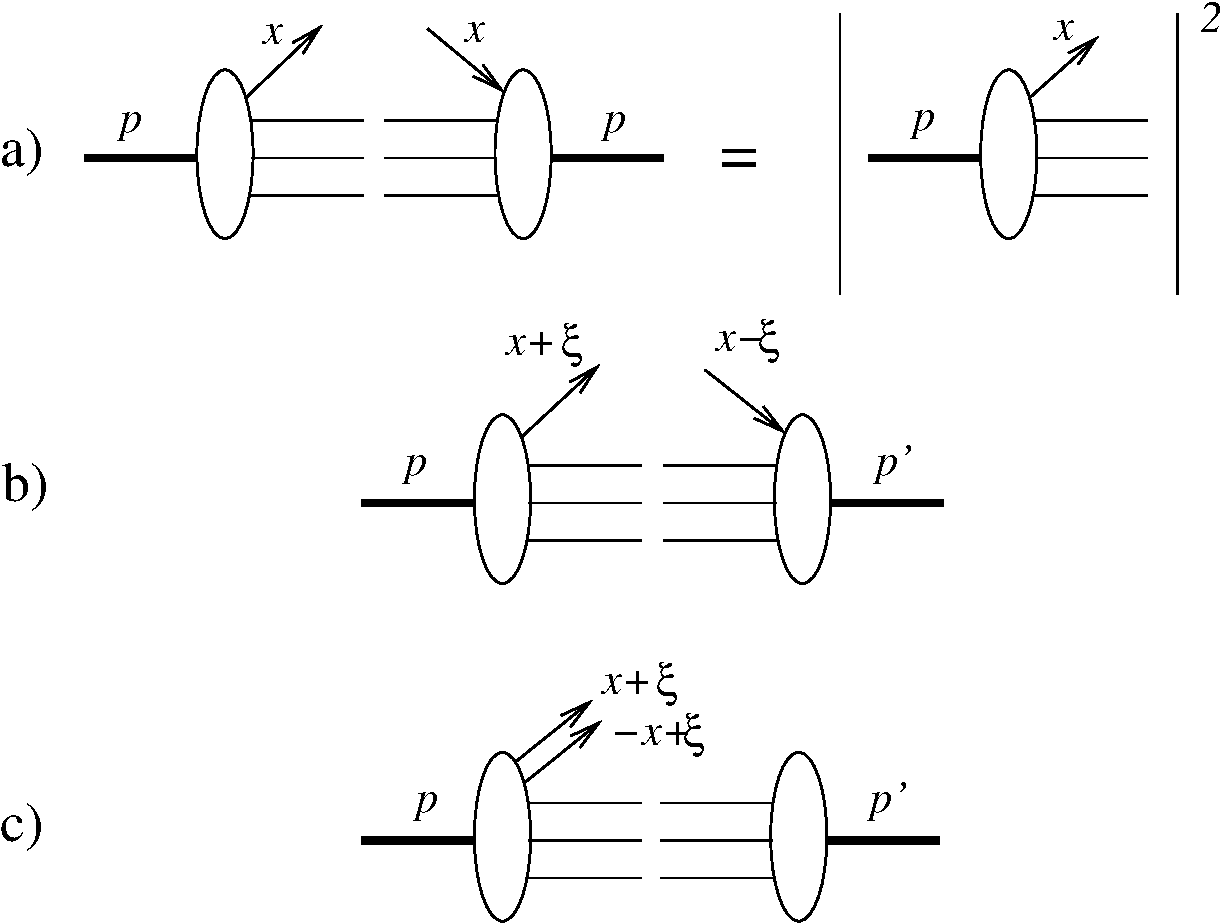
\includegraphics[height=6cm]{./figures/pdist_gpd_comparo.pdf}
\end{center}
\caption{\label{fig:pdis_gpd_comparo}
(a) Usual parton distribution, representing the probability to find a parton
with momentum fraction $x$ in the nucleon.
(b) GPD in the region where it represents the emission of a parton with
momentum fraction $x+\xi$ and its reabsorption with momentum fraction $x-\xi$.
(c) GPD in the region where it represents the emission of a quark-antiquark
pair, and has no counterpart in the usual parton distributions.
This figure has been adapted from Ref. \cite{Di00}.
}
\end{figure}

Apart from the momentum fraction variables $x$ and $\xi$, GPDs depend on the
four momentum transfer $t$.  This is an independent variable, because the
momenta $p$ and $p'$ may differ in either their longitudinal or transverse
components.  GPDs thus interrelate the longitudinal and transverse momentum
structure of partons within a fast moving hadron.

In order to access the physics contained within GPDs, one is restricted to the
hard scattering regime.  An important feature of hard scattering reactions is
the possibility to separate clearly the perturbative and nonperturbative stages
of the interaction.  Qualitatively speaking, the presence of a hard probe
allows one to create small size quark-antiquark and gluon configurations, whose
interactions are described by perturbative QCD (pQCD).  The non-perturbative
stage of the reaction describes how the hadron reacts to this configuration, or
how this probe is transformed into hadrons.  This separation is the so-called
factorization property of hard reactions.  Deep Exclusive Meson
electro-Production (DEMP) was first shown to be factorizable in
Ref. \cite{Co97}.  This factorization applies when the virtual photon is
longitudinally polarized, which is more probable to produce a small size
configuration compared to a transversely polarized photon.

GPDs are universal quantities and reflect the structure of the nucleon
independently of the reaction which probes the nucleon.  At leading twist-2
level, the nucleon structure information can  be parameterized in terms of four
quark chirality conserving GPDs, denoted $H$, $E$, $\tilde{H}$ and $\tilde{E}$.
$H$ and $E$ are summed over quark helicity, while $\tilde{H}$ and $\tilde{E}$
involve the difference between  left and right handed quarks.  $H$ and
$\tilde{H}$ conserve the helicity of the proton, while $E$ and $\tilde{E}$
allow for the possibility that the proton helicity is flipped.  Because quark
helicity is conserved in the hard scattering regime, the produced meson acts as
a helicity filter.  In particular, leading order QCD predicts that vector meson
production is sensitive only to the unpolarized GPDs, $H$ and $E$, whereas
pseudoscalar meson production is sensitive only to the polarized GPDs,
$\tilde{H}$ and $\tilde{E}$.  In contrast, deeply virtual Compton scattering
(DVCS) depends at the same time on both the polarized ($\tilde{H}$ and  
$\tilde{E}$) and the unpolarized ($H$ and $E$) GPDs.  This makes DEMP
reactions complementary to the DVCS process, as it
provides an additional tool to disentangle the different GPDs \cite{Go01}.

Besides coinciding with the parton distributions at vanishing momentum transfer
$\xi$, the GPDs have interesting links with other nucleon structure quantities.
Their first moments are related to the elastic form factors of the nucleon
through model-independent sum rules \cite{Ra00}:
\begin{eqnarray}
\sum_q e_q \int^{+1}_{-1} dx H^q(x,\xi,t) = F_1(t),\\
\sum_q e_q \int^{+1}_{-1} dx E^q(x,\xi,t) = F_2(t),\\
\sum_q e_q \int^{+1}_{-1} dx \tilde{H}^q(x,\xi,t) = G_A(t),\\
\sum_q e_q \int^{+1}_{-1} dx \tilde{E}^q(x,\xi,t) = G_P(t),
\end{eqnarray}
where $e_q$ is the charge of the relevant quark, $F_1(t)$, $F_2(t)$ are the
Dirac and Pauli elastic nucleon form factors, and $G_A(t)$, $G_P(t)$ are the
isovector axial and pseudoscalar nucleon form factors.  The $t$-dependence of
$G_A(t)$ is poorly known, and although $G_P(t)$ is an important quantity, it
remains highly uncertain because it is negligible at the momentum transfer of
$\beta$-decay\cite{Th01}.  Because of partial conservation of the axial current
(PCAC), $G_P(t)$ alone
receives contributions from $J^{PG}=0^{--}$ states\cite{Ma69}, which are the
quantum numbers of the pion, and so $\tilde{E}$ contains an important pion pole
contribution (Fig. 2a).

\begin{figure}[hbtp!]
\begin{center}
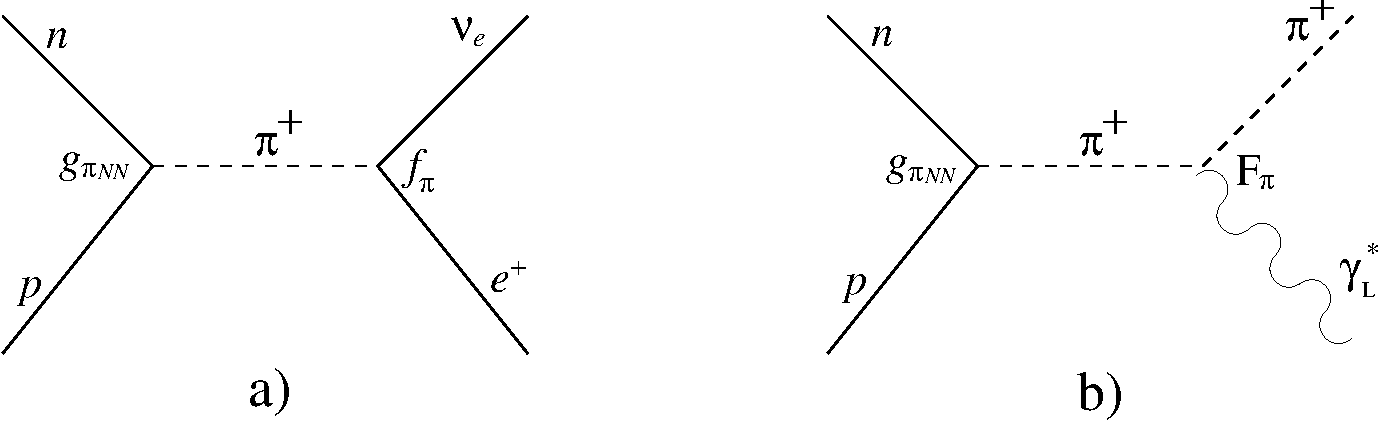
\includegraphics[height=4cm]{figures/PCAC_pion_pole.pdf}
\end{center}
\caption{\label{fig:PCAC_pion_pole}
(a) Pion pole contribution to $G_P(t)$, and hence to $\tilde{E}$.
(b) Pion pole contribution to meson electroproduction at low $-t$.
}
\end{figure}

Accordingly, Refs. \cite{Pe00,Be01} have adopted the pion pole-dominated
ansatz
\begin{equation}
\tilde{E}^{ud}(x,\xi,t) = F_{\pi}(t)\frac{\theta (\xi>|x|)}{2\xi
}\phi_{\pi}(\frac{x+\xi}{2\xi}),
\end{equation}
where $F_{\pi}(t)$ is the pion electromagnetic form factor, and $\phi_{\pi}$ is
the pion distribution amplitude.

$\tilde{E}$ cannot be related to already known parton distributions,
and so experimental information about $\tilde{E}$ via DEMP 
can provide new information on nucleon structure which is
unlikely to be available from any other source.

\begin{figure}[hbt!]
\begin{center}
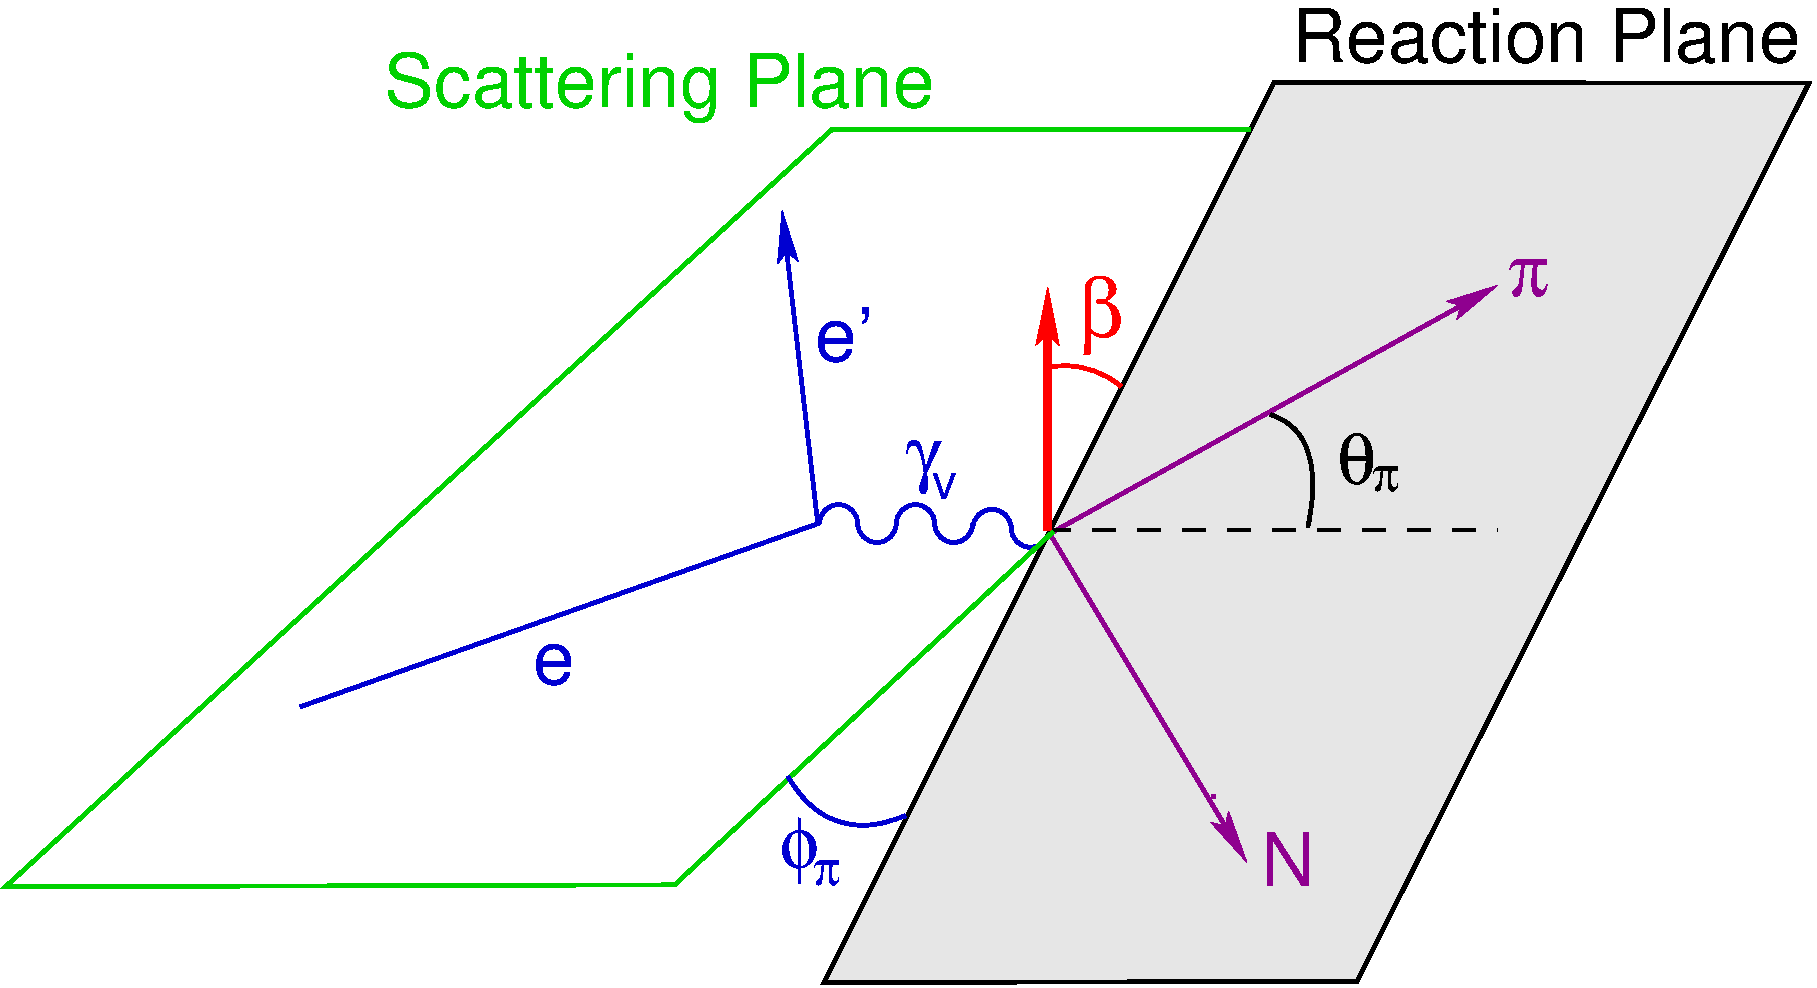
\includegraphics[height=5cm]{./figures/atpi_planes.pdf}
\end{center}
\caption{\label{fig:planes}
Scattering and hadronic reaction planes for exclusive $\vec{N}(e,e'\pi)N'$.
$\beta$ is the angle between the target nucleon polarization vector and the
reaction plane.  Some works alternatively label this angle as $(\phi-\phi_s)$.
}
\end{figure}

\subsection{Single spin asymmetry in exclusive pion electroproduction}

Frankfurt et al. \cite{Fr99} have considered a specific polarization observable
which is the most sensitive observable to probe the spin-flip $\tilde{E}$.
This variable is the single-spin asymmetry for exclusive charged pion
production, $\vec{p}(e,e'\pi^+)n$ or $\vec{n}(e,e'\pi^-)p$, from a transversely
polarized nucleon target, and is defined \cite{Be01} as
\begin{equation} \label{eqn:asy}
A_L^{\perp}=(\int^{\pi}_0 d\beta \frac{d\sigma^{\pi}_L}{d\beta} -
\int^{2\pi}_{\pi} d\beta \frac{d\sigma^{\pi}_L}{d\beta})
(\int^{2\pi}_0 d\beta \frac{d\sigma^{\pi}_L}{d\beta})^{-1},
\end{equation}
where $d\sigma^{\pi}_L$ is the exclusive charged pion electroproduction cross
section using longitudinally polarized photons and $\beta$ is the angle between
the nucleon polarization vector and the reaction plane (Fig.~\ref{fig:planes}).  
Frankfurt et al. \cite{Fr99} have shown that this asymmetry must vanish if
$\tilde{E}$ is zero.  If $\tilde{E}$ is not zero, the asymmetry will display a
sin$\beta$ dependence.  Their predicted asymmetry using the $\tilde{E}$ ansatz
from Ref. \cite{Va99} is shown in Fig. \ref{fig:frankfurt_atpi}.  This
calculation is $Q^2$-independent, depending only on how well the soft
contributions cancel in the asymmetry.

\begin{figure}[hbt!]
\begin{center}
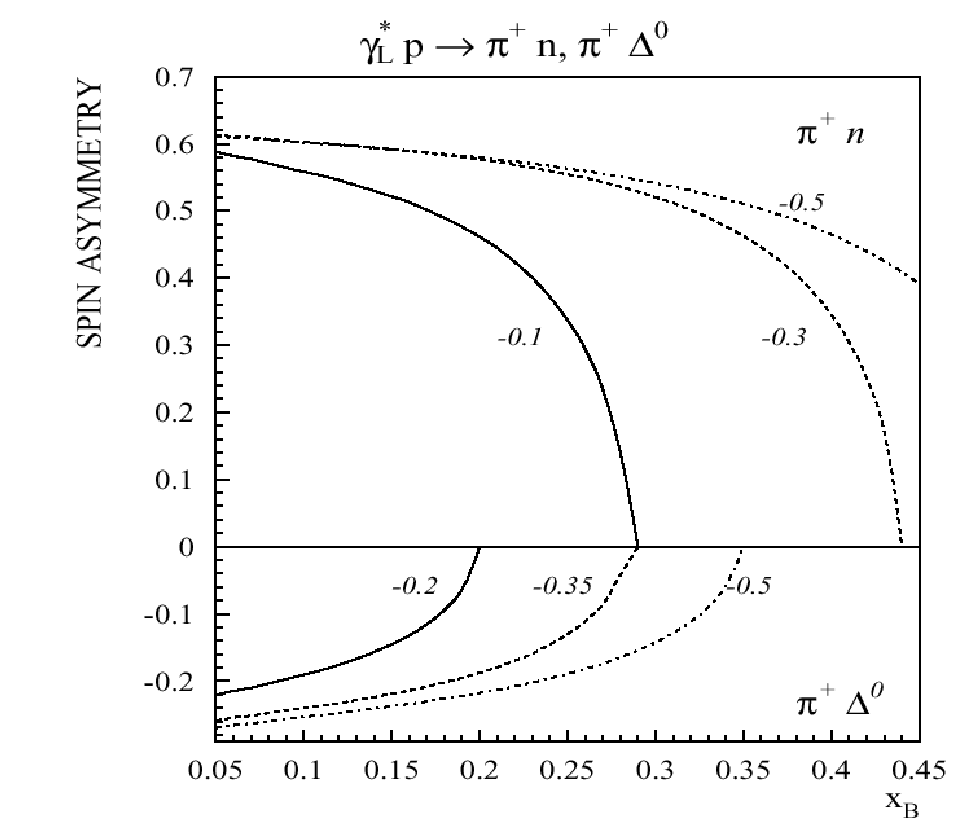
\includegraphics[height=7cm]{./figures/frankfurt_atpi.pdf}
\end{center}
\caption{\label{fig:frankfurt_atpi}
Transverse single-spin asymmetry for the longitudinal electroproduction of
$\pi^+n$ and $\pi^+\Delta^0$ at different values of $t$ [indicated on the
curves in GeV$^2$].  The asymmetry drops to zero at the parallel kinematic
limit, which is different for each $t$ value, because the definition of
$\beta$ is ill-defined at this point.  This figure is taken from
Ref. \protect{\cite{Fr00}}.
}
\end{figure}

It seems likely that a precocious factorization of the meson production
amplitude into three parts -- the overlap integral between the photon and pion
wave functions, the hard interaction, and the GPD -- will lead to a precocious
scaling of $A_L^{\perp}$ as a function of $Q^2$ at moderate $Q^2\sim 2-4$
GeV$^2$ \cite{Fr99}.  This precocious scaling arises from the fact that higher
order corrections, which are expected to be significant at low $Q^2$, will
likely cancel when one examines the ratio of two longitudinal observables.  In
contrast, the onset of scaling for the absolute cross section is only expected
for much larger values of $Q^2>10$ GeV$^2$.

\begin{figure}[hbt!]
\begin{center}
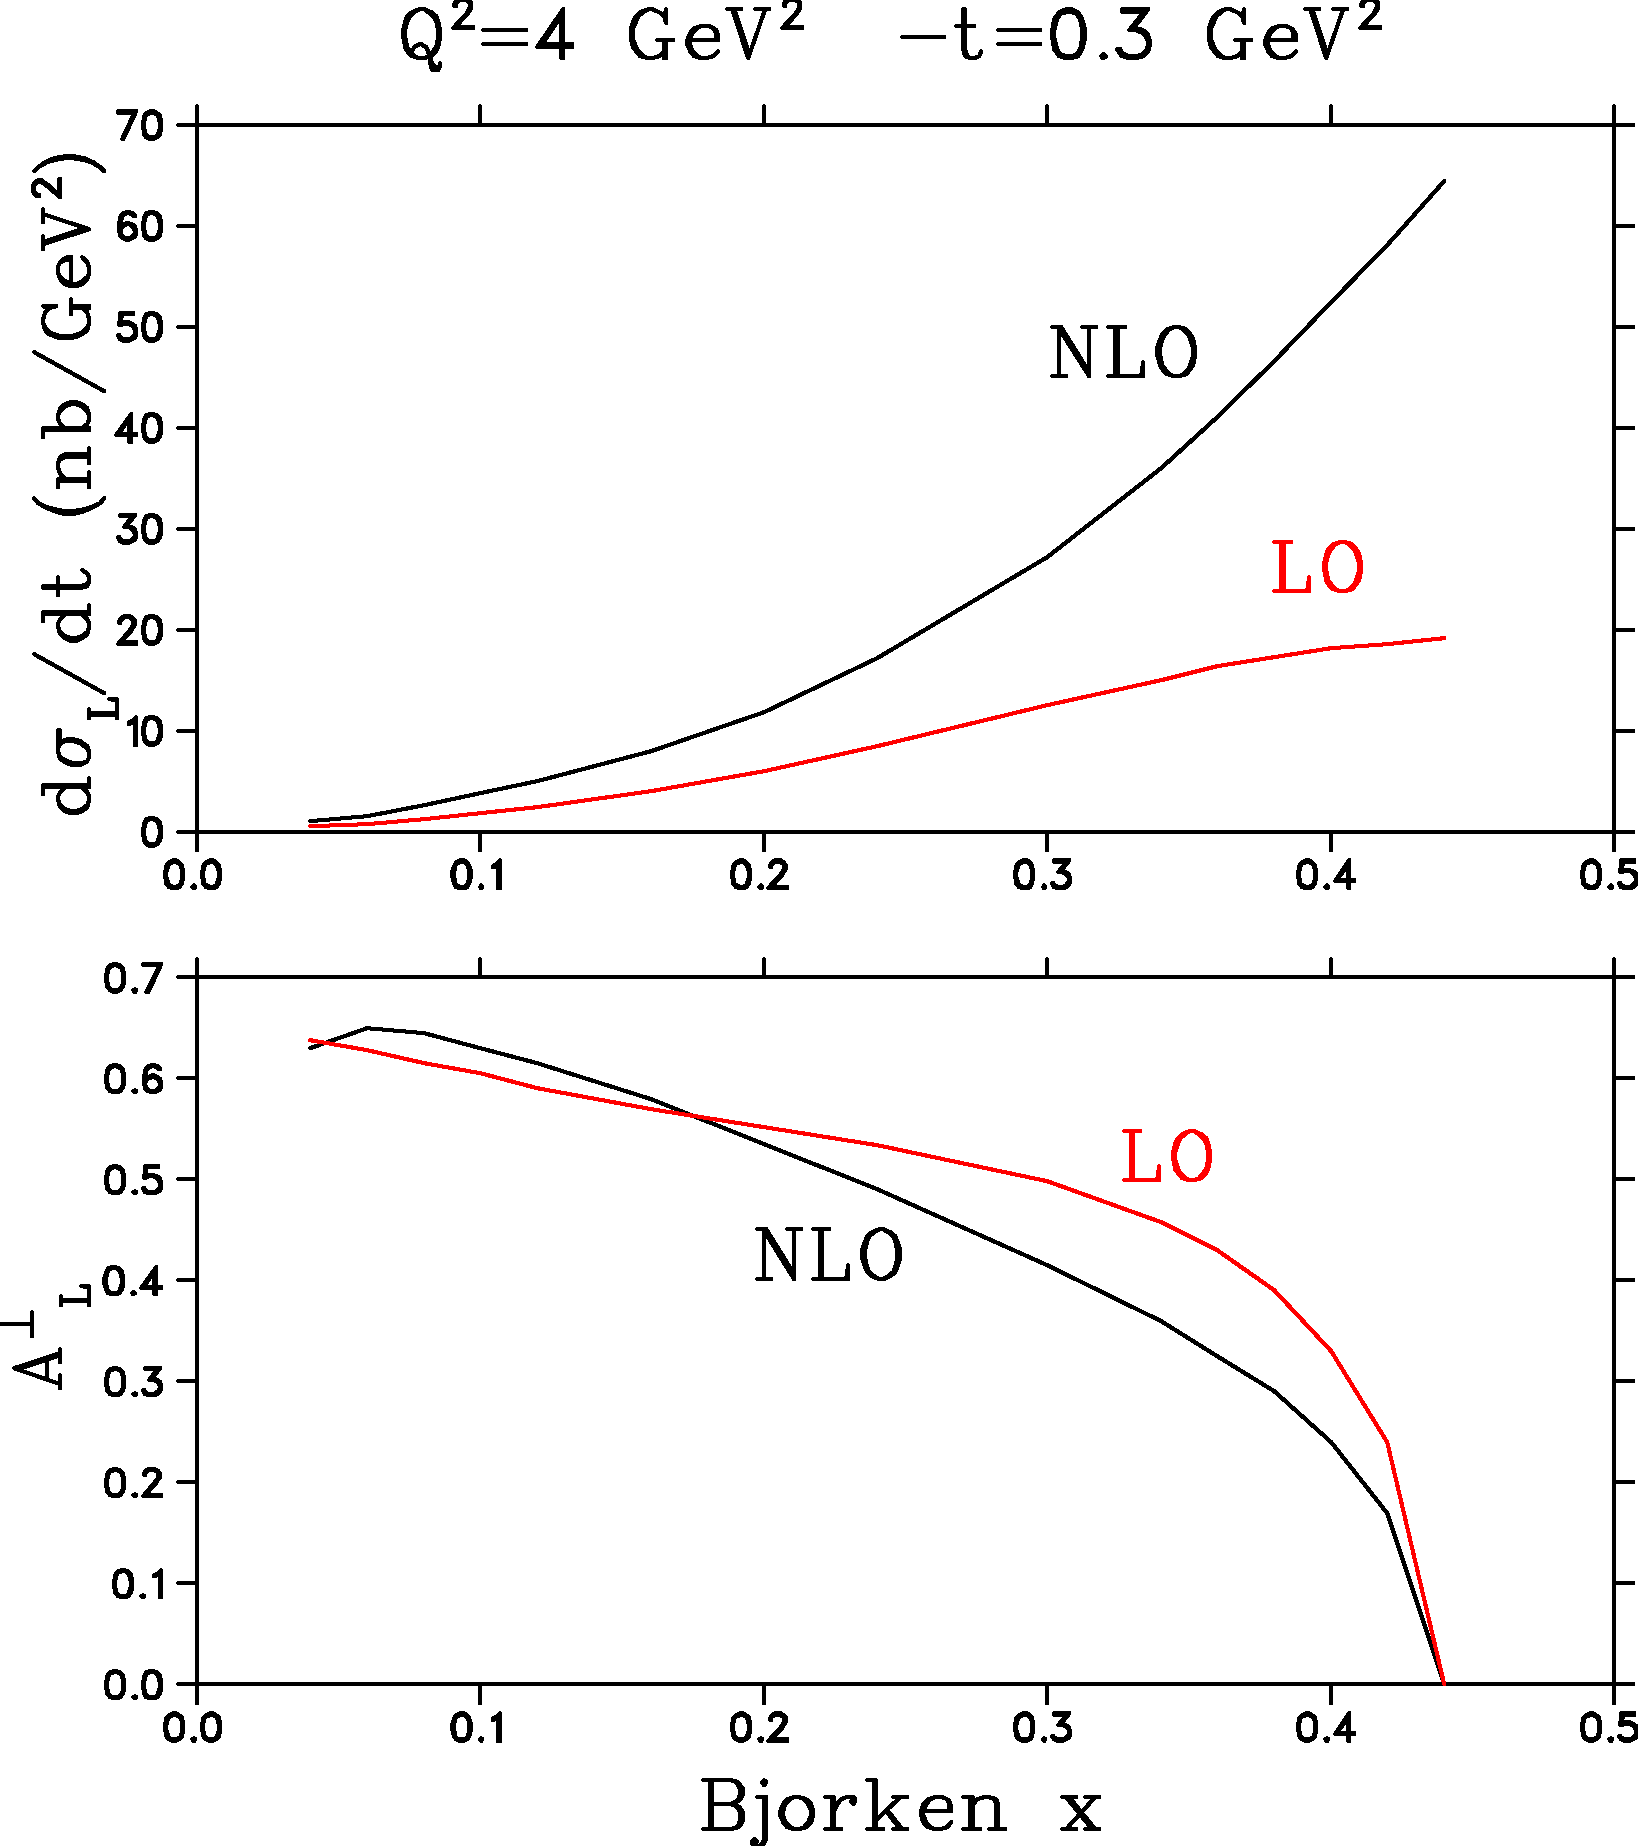
\includegraphics[height=10cm]{./figures/belitsky2.png}
\end{center}
\caption{\label{fig:belitsky_atpi}
Calculation of the longitudinal photon transverse nucleon spin asymmetry
including twist-four corrections by A. Belitsky \cite{belitsky} at $-t=0.3$
GeV$^2$, $Q^2$=4 GeV$^2$.  The red curves are the leading order calculation,
while the black curves have twist-four power effects taken into account.  While
the cross section is very sensitive to these corrections, the transverse spin
asymmetry is stable.}
\end{figure}

This point is made clear in Fig. \ref{fig:belitsky_atpi}.  This figure shows
renormalon model calculations \cite{belitsky} of both the asymmetry and the
longitudinal cross section at $Q^2=4$ GeV$^2$.  While the magnitude of the
cross section changes significantly when taking into account the twist-four
corrections, $A_L^{\perp}$ is essentially insensitive to them and displays the
expected precocious scaling.  The relatively low value of $Q^2$ for the
expected onset of precocious scaling is important, because it will be
experimentally accessible after the Jefferson Lab 12 GeV upgrade.  This places
$A_L^{\perp}$ among the most important GPD measurements that can be made in the
meson scalar.  If precocious scaling cannot be experimentally demonstrated in
this ratio of two cross sections, then it may not be possible to determine
GPDs from DEMP data.

Refs. \cite{Go01} and \cite{Fr00} also point out that the study of the
transverse target single-spin asymmetry versus $t$ is important for the
reliable extraction of the pion form factor from electroproduction experiments
(Fig. 2b).  Investigations of hard exclusive $\pi^+$ electroproduction using a
pQCD factorization model \cite{Ma99,Ca90} find that at $x_B=0.3$ and
$-t=-t_{min}$, the pion pole contributes about 80\% of the longitudinal cross
section.  Since the longitudinal photon transverse single-spin asymmetry is an
interference between
pseudoscalar and pseudovector contributions, its measurement would help
constrain the non-pole pseudovector contribution, and so assist the more
reliable extraction of the pion form factor.  The upper $Q^2=6$ GeV$^2$ limit
of the approved pion form factor measurements in the JLab 12 GeV program
\cite{12GeV} is dictated primarily by the requirement $-t_{min}<0.2$ GeV$^2$,
to keep non-pion pole contributions to $\sigma_L$ at an acceptable level
\cite{Ca90}.  Transverse target single-spin asymmetry studies versus $t$ may
eventually allow, with theoretical input, the use of somewhat larger $-t$ data
for pion form factor measurements, ultimately extending the $Q^2$-reach of pion
form factor data acquired with JLab 12 GeV beam.  Thus, measurements of
the transverse single-spin asymmetry are a logical step in the support of the
pion form factor program.

\subsection{The Complementarity of Separated and Unseparated Asymmetry
  Measurements}

The reaction of interest is $^3He(e,e'\pi^-)p(pp)_{sp}$.
The measurement of the transverse single-spin asymmetry requires the detection
of the $\pi^-$ in non-parallel kinematics.  It is the component of the target
polarization parallel to $\hat{q}\times\hat{p_{\pi}}$ that is important, and
this direction is uniquely defined only in non-parallel kinematics.

Experimentally, the angle between the target polarization and the reaction
plane, $\beta$, and the angle between the scattering and reaction planes,
$\phi$, are not independent.  If the target polarization is at some angle,
$\phi_s$, relative to the scattering plane, then $\beta = \phi_s-\phi$.  
The polarized nucleon cross section can be expressed \cite{Ba73} 
in terms of these variables as:
\begin{multline}\label{eqn:sigtarg}
\sigma_t =  - P_\perp \sin \beta \left[\sigma^y_{TT}+ 2\epsilon \; 
  \sigma^y_L \right] \\
- P_\perp \sin \beta \left[\epsilon (\cos 2\phi_s \cos 2\beta + 
  \sin 2\phi_s \sin 2\beta) \; \sigma^y_{TT'} \right]\\
- P_\perp \sin \beta \left[\sqrt{2\epsilon(1+\epsilon)}(\cos \phi_s \cos \beta 
  + \sin \phi_s \sin \beta) \; \sigma^y_{LT}\right] \\
-P_\perp \cos \beta \left[\sqrt{2\epsilon(1+\epsilon)}(\sin \phi_s \sin \beta 
  - \cos \phi_s \cos \beta)\; \sigma^x_{LT} \right]\\
-P_\perp \cos \beta \left[\epsilon (\sin 2\phi_s \sin 2\beta 
  - \cos 2\phi_s \cos 2\beta)  \; \sigma^x_{TT} \right] .
\end{multline}
From the above equation, it is clear that to extract $A_L^{\perp}$
it is necessary to first isolate the 
$\sin \beta$ Fourier component of the polarized nucleon cross section.
Once that has been accomplished, one must then separate the $\sigma_L^y$ term 
from the $\sigma_{TT}^y$ term via a Rosenbluth-type separation.

It has not yet been possible to perform an experiment to measure $A_L^{\perp}$.
The conflicting experimental requirements of transversely polarized target,
high luminosity, L--T separation, and closely controlled systematic
uncertainty, make this an exceptionally challenging observable to measure.  The
SHMS+HMS is the only facility with the necessary resolution and systematic
error control to allow a measurement of $A_L^{\perp}$.  However, the beamtime
required to do a good measurement with current polarized target technology is
in the range of 10$^3$ days.  To minimize the beamtime required, PR12-12-005
\cite{atpi39}
proposed the use of a next generation, externally polarized, continuous flow,
high luminosity $^3$He target based on a large volume polarizer and compressor
developed at the University of New Hampshire.  The science case
for this measurement was favorably reviewed by PAC39, and they encouraged the
continued development of the target technology.  Although the New Hampshire
group is making continued progress on the development of the target, there is
no timeline for its actual implementation at Jefferson Lab.

The most closely related measurement, of the transverse single-spin asymmetry
in exclusive $\pi^+$ electroproduction without an L--T separation, was
published by the HERMES Collaboration in 2010 \cite{hermes10}.  Their data were
obtained for average values of $\langle x_B \rangle =0.13$, $\langle Q^2 \rangle
=2.38$ GeV$^2$ and $\langle t' \rangle = -0.46$ GeV$^2$, subject to the
criterion $W^2>10$ GeV$^2$.  The six Fourier amplitudes in terms of the
azimuthal angles $\phi$, $\phi_s$ of the pion-momentum and proton-polarization
vectors relative to the lepton scattering plane were determined.  Of these, at
leading twist only the $\sin(\phi-\phi_s)_{UT}$ Fourier amplitude receives a
contribution from longitudinal photons.  If one assumes that longitudinal
contributions dominate, these $A_{UT}^{sin(\phi-\phi_s)}$ values can be
compared to GPD models for $\tilde{E}$, $\tilde{H}$.

\begin{figure}[hbt!]
\begin{center}
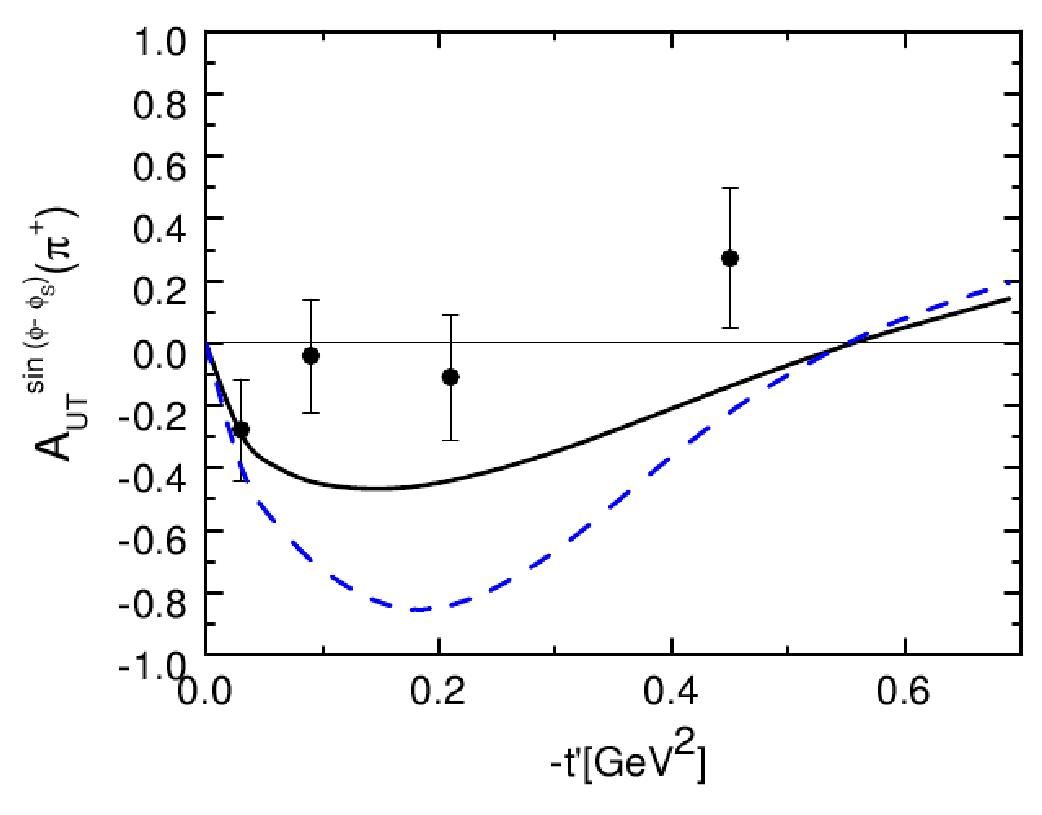
\includegraphics[height=7cm]{./figures/hermes_Aut.pdf}
\end{center}
\caption{\label{fig:hermes_aut}
Predictions by Goloskokov and Kroll for the sin$(\phi-\phi_s)$ moment of
$A_{UT}$ in the handbag approach, in comparison to the data from HERMES at
$Q^2=2.45$ GeV$^2$, $W=3.99$ GeV.  The independent variable is
$-t'=|t-t_{min}|$.  Dashed line: contribution from longitudinal photons only.
Solid line: full calculation including both transverse and longitudinal
photons.  This figure is taken from Ref. \protect{\cite{Go10}}.}
\end{figure}

Because transverse photon amplitudes are suppressed by $1/Q$, at very high
$Q^2$ it is safe to assume that all observed meson production is due to
longitudinal photons.  At the lower $Q^2$ typical of the JLab and HERMES
programs, however, this is not the case.  Calculations by Goloskokov and Kroll
\cite{Go10} indicate much of the unseparated cross section measured by HERMES
\cite{hermes10} is due to contributions from transversely polarized photons.
In addition, there are contributions to $A_{UT}^{sin(\phi-\phi_s)}$ from the
interference between two amplitudes, both for longitudinal photons, as well as
transverse photons~\cite{Di05}.  As indicated in Fig. \ref{fig:hermes_aut}, the
contribution from transverse photons tends to make the asymmetry smaller.  At
the HERMES kinematics, the dilution caused by transverse photons is about
50\%.

\begin{figure}[hbt!]
\begin{center}
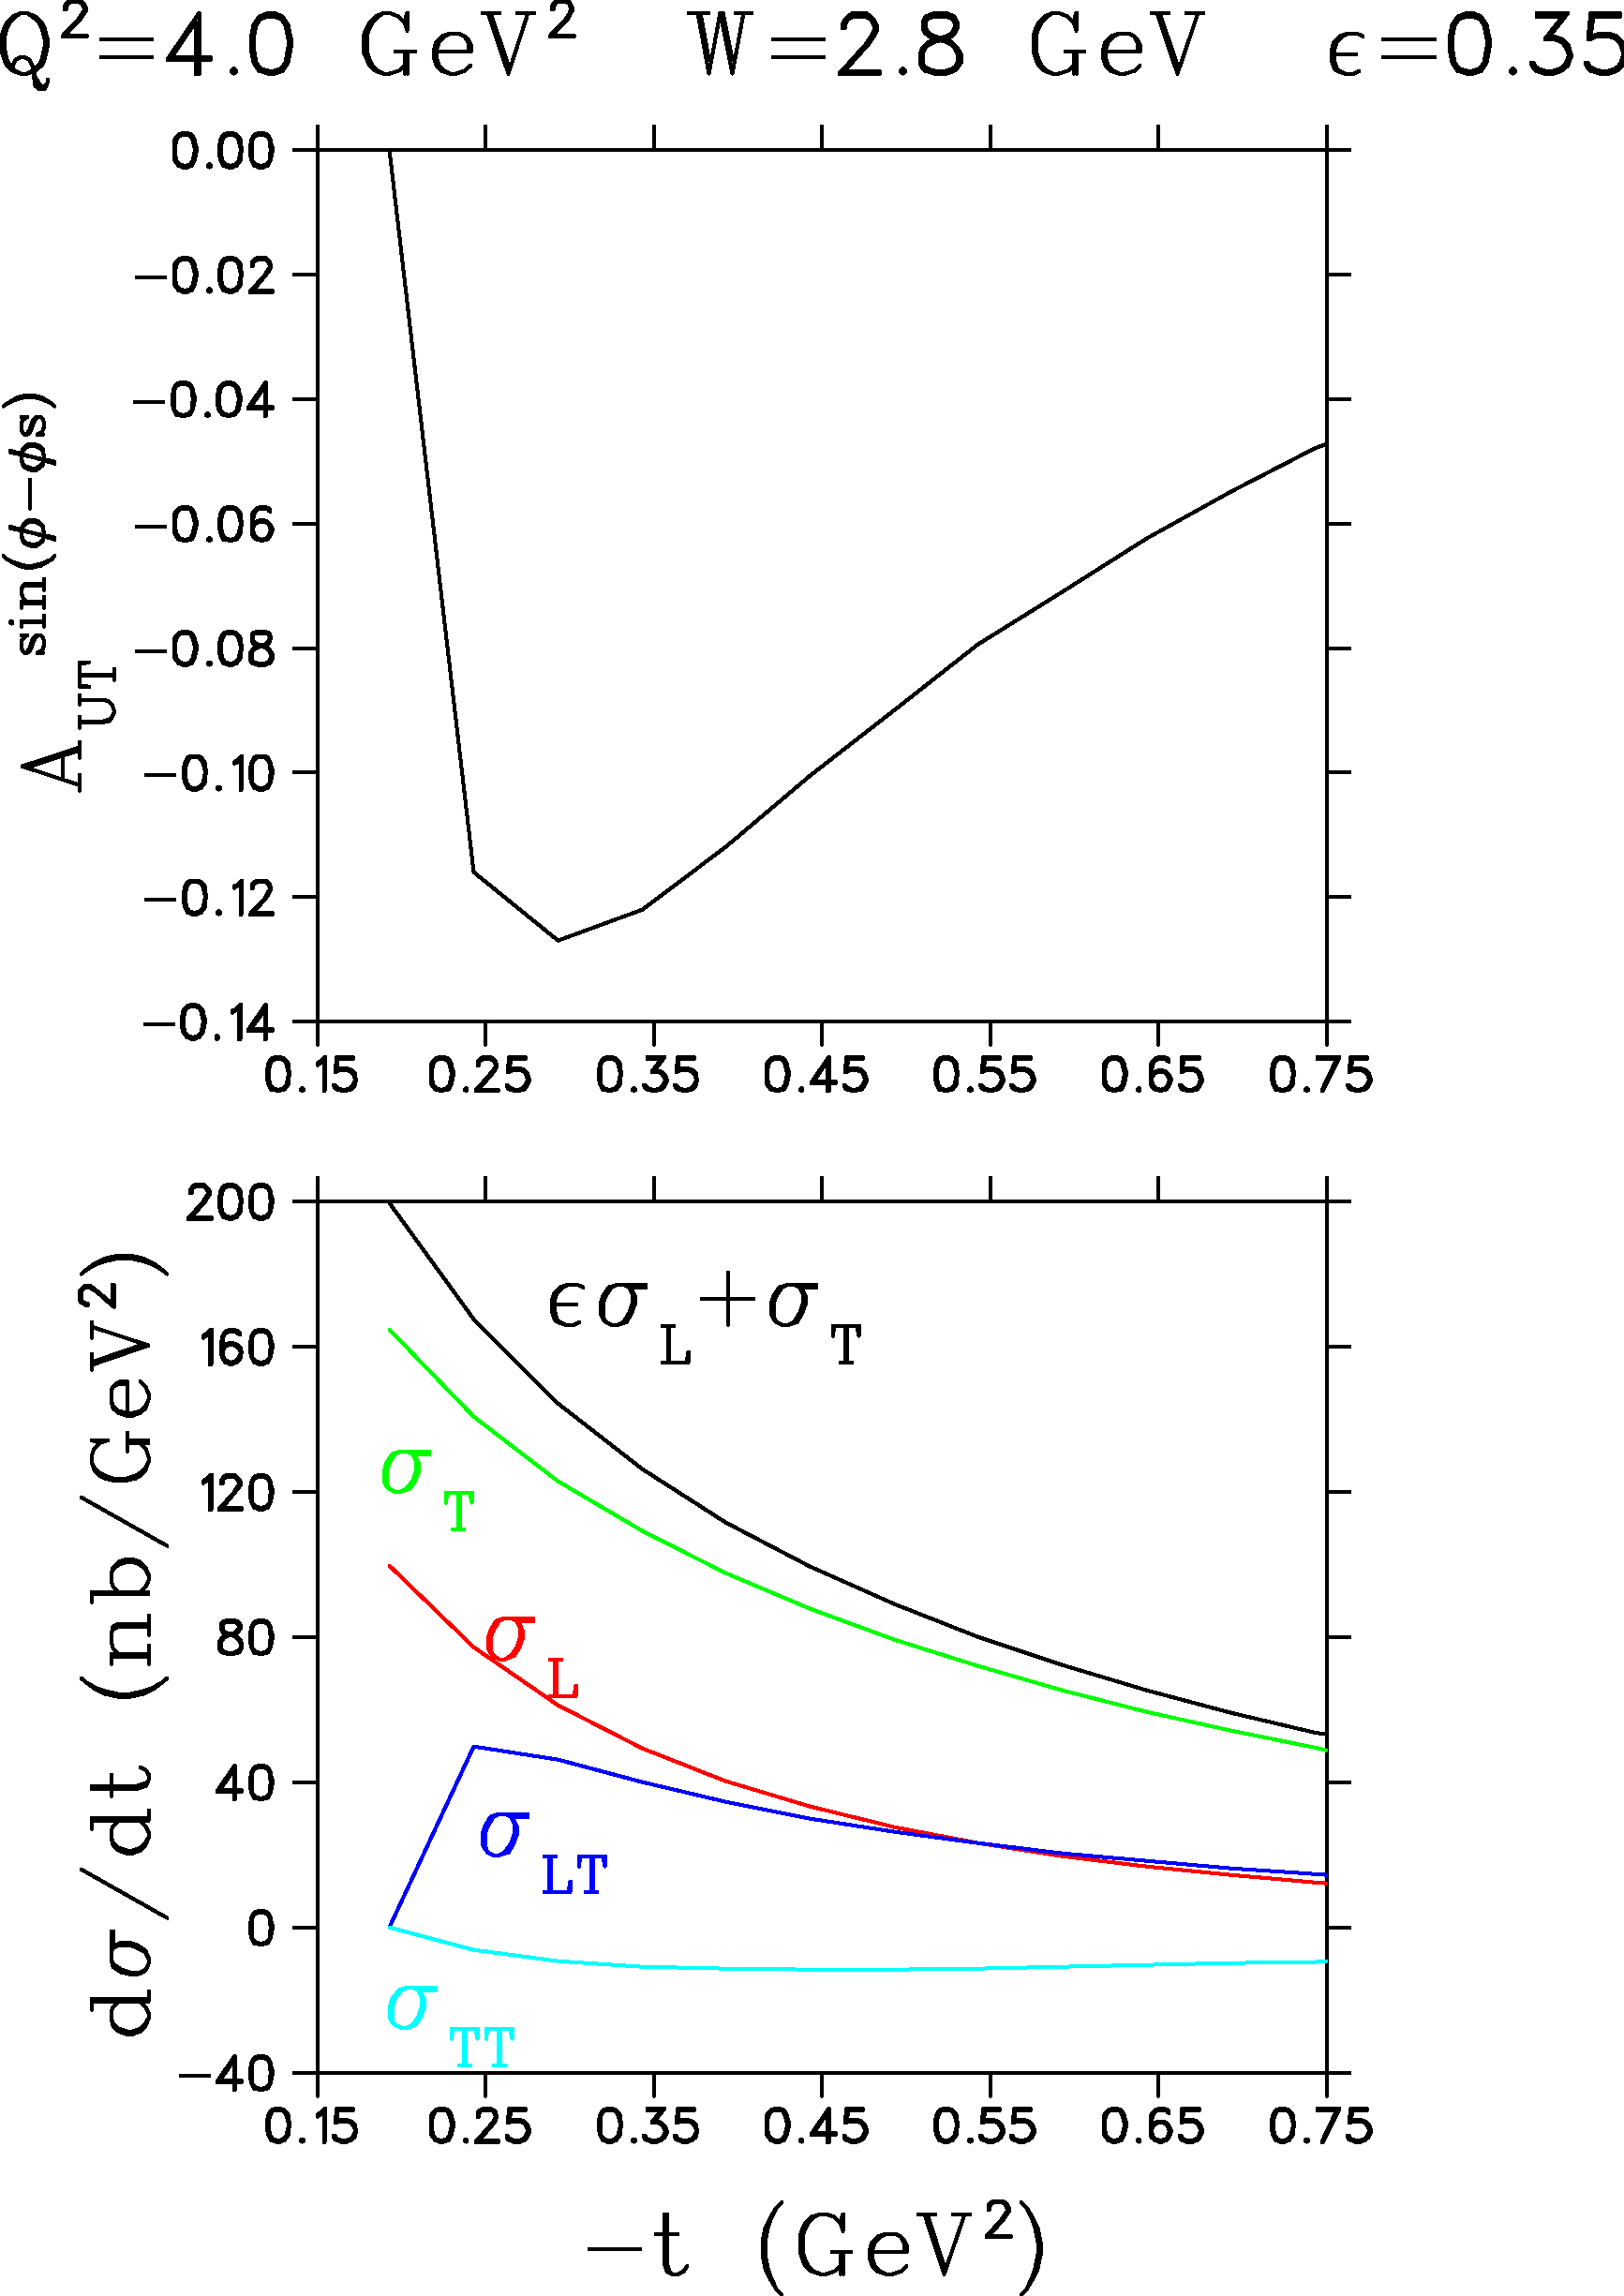
\includegraphics[height=10cm]{./figures/goloskokov2.png}
\caption{\label{fig:golo_aut}
Calculation of the cross section components and sin$(\phi-\phi_s)$ moment of
the transverse nucleon spin asymmetry $A_{UT}$ in the handbag approach by
Goloskokov and Kroll \cite{GoPC} for kinematics similar to those in
Fig. \ref{fig:belitsky_atpi}.  Our measurement will be at higher
$0.55<\epsilon<0.75$ than the $\epsilon=0.35$ kinematics of this figure,
so the dilution in the asymmetry will be significantly less.}
\end{center}
\end{figure}

A run-group proposal concurrent with the SoLID transversely polarized $^3$He
SIDIS experiment allows for an unseparated asymmetry measurement to be obtained
on a sooner timescale than the Hall C measurement.  In comparison to the HERMES
measurement, the experiment proposed here will probe higher $Q^2$ and $x_B$,
with much smaller statistical errors over a wider range of $-t$.
SoLID will allow the first measurement for $Q^2>4$ GeV$^2$, where GPD-based
calculations are expected to apply.  Thus, the measurements should be more
readily interpretable than those from HERMES.  Similar measurements using
CLAS-12 and a transversely polarized $^1$H target have been discussed
previously \cite{clas}, but this measurement will allow for smaller statistical
uncertainties, due to SoLID's higher luminosity capabilities.

Handbag model calculations by Goloskokov and Kroll \cite{GoPC} shed further
light on the expected asymmetry dilution.  The lower left panel of
Fig. \ref{fig:golo_aut} shows their predictions for the cross section
components in exclusive charged pion production.  Although their calculations
tend to underestimate the $\sigma_L$ values measured in the JLab $F_{\pi}-2$
experiment \cite{Fpi2}, their model is in reasonable agreement with the
unseparated cross sections \cite{Go10}.  They predict significant transverse
contributions for JLab kinematics.  A comparison of the unseparated asymmetry
at $-t=0.3$ GeV$^2$, $x_B=0.365$ in Fig. \ref{fig:golo_aut} with the separated
longitudinal asymmetry at the same values of $x_B$, $-t$ in
Fig. \ref{fig:belitsky_atpi} indicates a substantial dilution of the
unseparated asymmetry due to transverse photon contributions, similar to that
observed in Fig. \ref{fig:hermes_aut}.

In addition to allowing a measurement at $Q^2>4$ GeV$^2$, a measurement by
SoLID of $A_{UT}^{sin(\phi-\phi_s)}$ will cover a fairly large range of $-t$,
allowing the asymmetry to be mapped over its full range with good statistical
uncertainties -- from its required zero-value in parallel kinematics, through
its maximum, and then back to near-zero as $\sigma_T$ dominates $\sigma_L$ at
larger $-t$.  The shape of the asymmetry curve versus $-t$, as well as its
maximum value, are critical information for comparison to GPD-based models.  At
a later date, the New Hampshire polarized target might enable a measurement of
$A_L^{\perp}$ in Hall C.  The
comparison of the maxima and $t$-dependences of both measurements will provide
complementary data needed to extract $\tilde{E}$ information and better
understand non-pole contributions complicating the extraction of the pion form
factor from electroproduction data.


\newpage
\section {Experimental setup}
We propose to carry out the new measurement using the Soenoidal Large Intensity Device (SoLID~\cite{solid_pcdr}), in parallel with the already approved experiment, E12-10-006~\cite{solid:e12-10-006}, which will measure the Semi-Inclusive Deep-Inelastic Scattering (SIDIS). There are two SoLID configurations, called the SoLID-SIDIS and SoLID-PVDIS. Besides E12-10-006, two SIDIS experiments, E12-11-007~\cite{solid:e12-11-007} and E12-11-108~\cite{solid:e12-11-108}, along with the $J/\psi$ experiment (E12-12-006~\cite{solid:e12-12-006}), will use the SoLID-SIDIS configuration. All these experiments have been approved with A or A- rating. In addition, two "bonus-run" experiments, E12-10-006A~\cite{solid:e12-10-006A} and E12-11-108A~\cite{solid:e12-11-108A}, have also been approved to run in parallel with the SIDIS experiments. The SoLID-PVDIS configuration is for the Parity Violation in Deep Inelastic Scattering (PVDIS).

The experiment will use a near identical setup as E12-10-006, but with few additions without affecting the approved experiment. We will use exactly the same online production trigger, which is the coincidence of electron triggers and hadron triggers. However, we request to add a new trigger type on top of the existing ones to identify the proton events for the offline triple coincidence analysis. The SoLID-SIDIS detector can only detect protons with scattering angles from 8$^{\circ}$ up to 24$^{\circ}$, while the main proton events from the DVMP process can cover up to 65$^{\circ}$. We propose to add a new proton detector based on scintillator counters  to detect protons from  24$^{\circ}$ to  65$^{\circ}$. The new detector will be placed between the target system and the entrance and of CLEO-II magnet. The new proton trigger and the new proton detector will be discussed in more detailed in the following sections.

\subsection {Transversely Polarized $\mathrm{^{3}He}$ Target}
\begin{table}[!ht]
\centering
\begin{tabular}{|c|c|}
\hline
Target                       & $^3$He              \\\hline 
Length                       & 40 cm               \\\hline          
Target Polarization          & $\sim$60\%          \\\hline 
Target Spin Flip             & $\leq$20 mins       \\\hline 
Target Dilution              & 90\%  \\\hline
Effective Neutron            & 86.5\%  \\\hline
Target Polarimetry Accuracy  & $\sim$ 3\%          \\\hline
\end{tabular}
\caption{\footnotesize{Key Parameters of the $\mathrm{^{3}He}$ target.}}\label{table:target}
\end{table} 
The proposed measurement will utilize the same polarized $\mathrm{^{3}He}$ as E12-10-006~\cite{e12-10-006}. Such a target was successfully employed in E06-110, a 6~GeV SIDIS experiment in Hall A. The polarization direction is held by three sets of Helmholtz coils with a 25~Gauss magnetic filed. Both the transverse and longitudinal directions can be provided by rotating the magnetic field. The $\mathrm{^{3}He}$ gas with density of about 10~atm (at $0^{\circ}$) is stored in a 40~cm target cell made of thin glasses. With a 15~$\mu A$ electron beam, the neutron luminosity can be as high as $10^{36} cm^{-2}s^{-1}$. The in-beam polarization of 60\% was archived during the E06-110 experiment. Two kinds of polarimetry, NMR and EPR, were used to measure the polarization with relative 5\% precision. We have planed to improve the accuracy of the measurement to reach 3\%.

The target spin will be reversed for every 20 minutes by using the RF AFP technique. The additional polarization loss due to the spin reversal was kept at $<10~\%$ which has been taken into account in the overall 60\% in-beam polarization. A new method for spin reversal using filed rotation has been tested and was able to eliminate the polarization loss. Such an improvement will enable us to perform the spin-reversal in few minutes to reduce the target-spin-correlated systematic errors. The key parameters of the $\mathrm{^{3}He}$ target are summarized in Table~\ref{table:target}.
  
A collimator, similar to the one used in the E06-110, will be placed next to the target cell window to minimize the target cell contamination and to reduce the event rate. Several calibration targets will also be installed in this target system, including a multi-foil $^{12}C$ for optics study, a BeO target for beam tuning, and a reference target cell for dilution study and other calibration purposes.
  
\subsection {SoLID Spectrometer and Detectors} 
The solenoid magnet for SoLID will be based on the CLEO-II magnet built by Cornell University. The magnet is 3 meters long with the out diameter of 3 meters and the inner diameter of 1 meter. The field strength is greater than 1.35 Tesla with integrated BDL of 5 Tesla-meters. The fringe filed at the front end after shielding is less than 5 Gauss. In the SIDIS-configuration, the CLEO-II magnet provides 2$\pi$ acceptance in the azimuthal angle ($\phi$) and covers the polar angle ($\theta$) from 8$^{\circ}$ up to 24$^{\circ}$. The momentum acceptance is between 0.8 and 7.5~GeV/c and the resolution is about 2\%. 

\begin{figure}[!ht]
 \begin{center}
  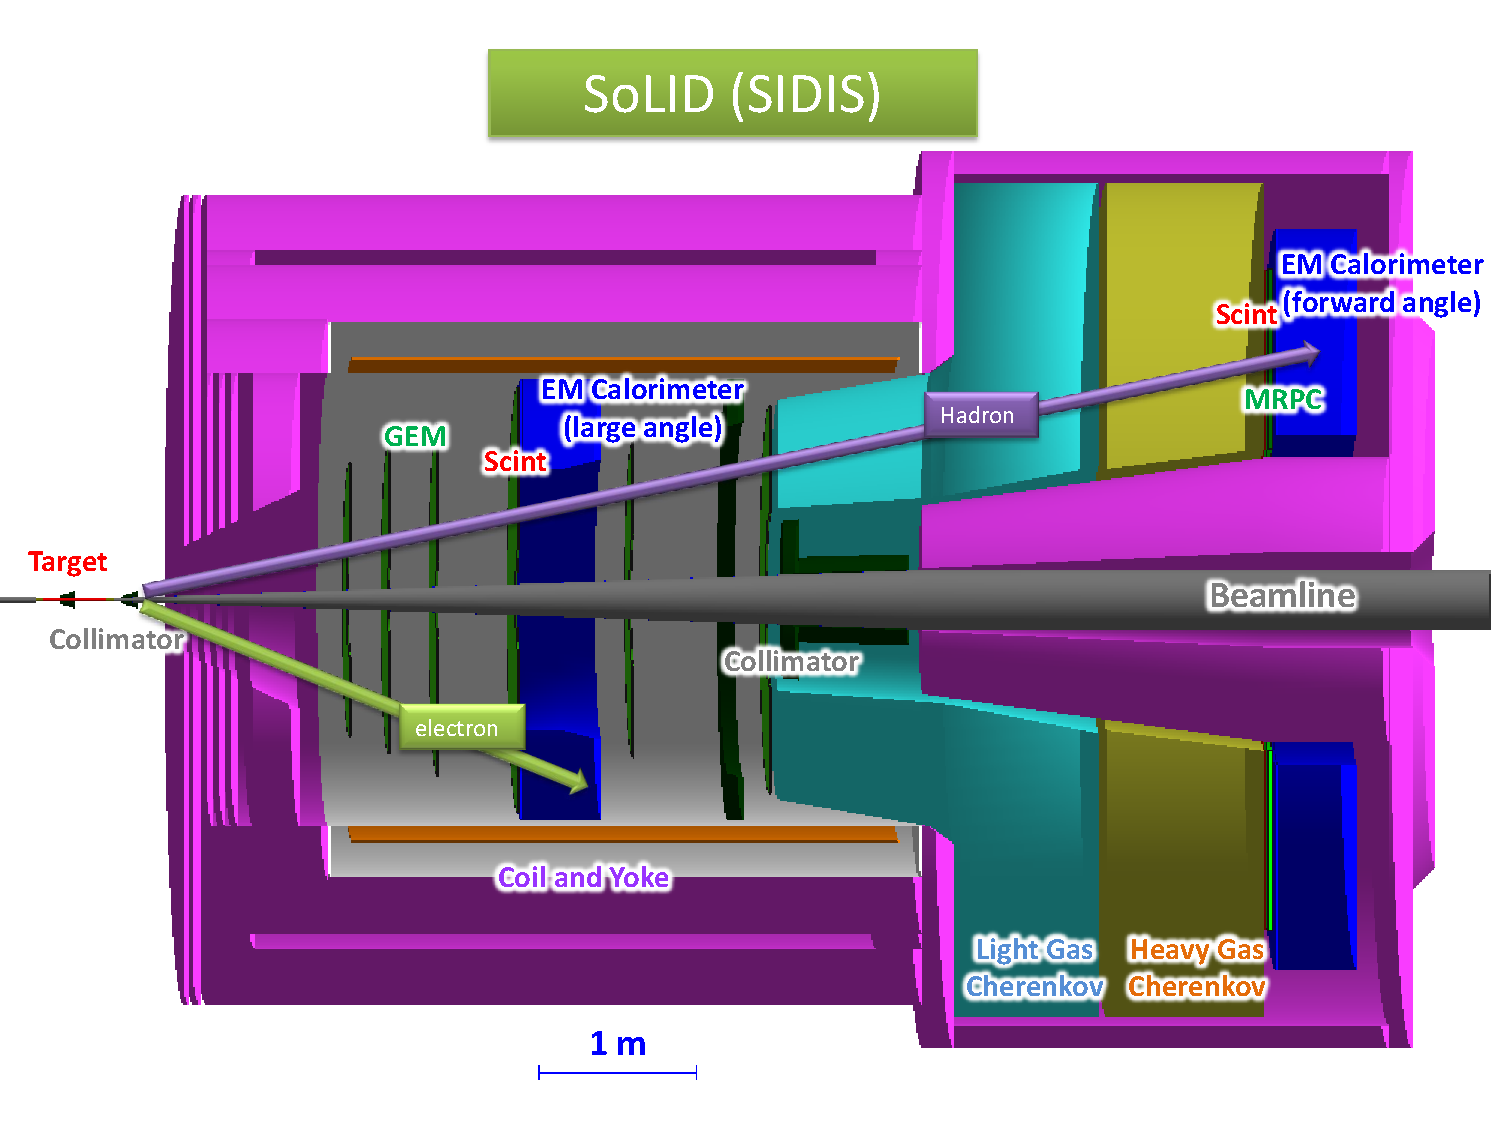
\includegraphics[width=0.8\textwidth]{./figures/SoLID_SIDIS_setup.pdf}
   \caption[The Detector Layout of the SoLID-SIDIS configuration]{\footnotesize{The Detector Layout of the SoLID-SIDIS configuration. The detector system includes six Gas Electron Multiplier (GEM) planes for charged particle tracking, two Scintillator Pad Detectors (SPD) followed by two Shashlyk sampling EM Calorimeters (EC) for energy measurement and particle identification, a Light Gas \v{C}erenkov Detector (LGC) for e-$\pi^{\pm}$ separation, a Heavy Gas \v{C}erenkov Detector (HGC) for $\pi^{\pm}$-$K^{\pm}$ separation, as well as a Multi-gap Resistive Plate Chamber (MRPC) for timing measurement. The first four GEM trackers, the first SPD (i.e. LASPD) and EC (i.e. LAEC) form the large-angle detection system for electron measurement. The forward-angle detection system, to measure electron and hadrons, is composed of all six GEM trackers, LGC, HGC, MRPC, the second SPD (i.e. FASPD) and the second EC (FAEC). The photon-detection in the large-angle is given by the veto-signal of the SPD in coincidence with the EC signal, where the photons in the forward-angle system will be triggered by the EC signal plus the veto-signals of LGC, SPD, and MRPC.}}
   \label{solid_sidis}
 \end{center}
\end{figure}

The layout of the SoLID detectors in the SIDIS-configuration is shown in Fig.~\ref{solid_sidis}. The detector system is divided into two regions for the forward-angle (FA) detection and the large-angle (LA) detection. Six Gas Electron Multiplier (GEM) tracking chambers will be used for charged particle tracking, where only the first four of them will be used for the large-angle detection. In each region, a Shashlyk-type sampling EM calorimeter (LAEC or FAEC) will measure the particle energy and identify electrons from hadrons. A scintillator-pad detector (LASPD and FASPD) will be installed in front of each EC to reject photons and provide timing information. The forward-angle detectors will detect both the electrons and hadrons (mainly $\pi^{\pm}$). A light-gas \v{C}erenkov detector (LGC) and a heavy-gas \v{C}erenkov detector (HGC) will perform the $e/\pi^{\pm}$ and $\pi^{\pm}/K^{\pm}$ separation, respectively. The Multi-gas Resistive Plate Chamber (MRPC) will provide a precise timing measurement and serve as a backup of the FASPD on photon rejection. A more detailed discussion of the design, simulation, prototype-test of each detector is given in the SoLID preliminary conceptual design report (pCDR)~\cite{solid_pcdr}. 

Table~\ref{table:key_par_sidis_dvcs} summarizes the key parameters of the detector system in the SIDIS configuration for both the SIDIS and DVMP measurements. 
\begin{table}\centering
\begin{tabular}{|c|c|c|c|c|}
\hline
Experiments                             & SIDIS                 & DVMP  \\\hline
Reaction channel                     &  $\vec{n}(e,e'\pi^{\pm})X$    & $\vec{n}(e,e'\pi^{-})p$	\\\hline
Target                                       & $^3$He                &same 	\\\hline
Unpolarized luminosity             & $\sim10^{37}$ cm$^{-2}$s$^{-1}$ per nucleon        & same	\\\hline 
Momentum coverage   & 0.8-7.5 (GeV/c)               &same 	\\\hline
Momentum resolution              &  $\sim$2\%            & same\\\hline
Azimuthal angle coverage      & 0$^{\circ}$ ~360$^{\circ}$                  & same	\\\hline
Azimuthal angle resolution      & 5 mr                  & same	\\\hline
Polar angle coverage              &  8$^{\circ}$-24$^{\circ}$ for $e$                 &  same \\\hline
Polar angle coverage              &  8$^{\circ}$-14.8$^{\circ}$ for $\pi^{\pm}$  &  same 	\\\hline
				                                 &                                                        & 8$^{\circ}$-24 $^{\circ}$ for $p$         \\\hline
   				                                 &                                                        & 24$^{\circ}$-65 $^{\circ}$ for $p$ with recoil detector         \\\hline
 Polar angle resolution             & 0.6 mr                & same	\\\hline
Target Vertex resolution          & 0.5~cm                & same \\\hline
 Energy resolution on ECs      & 5\%$\sim$10\%         & same   \\\hline
Trigger type                             & Double Coincidence $e^-+\pi^{\pm}$ & Tripple Coincidence $e^-+\pi^{-}+p$\\\hline
Expected DAQ rates               &  $<$100 kHz           &  same online ($<$30 Hz offline)\\\hline
Main Backgrounds                  & (e,e'K$^\pm$)        &(e,e'$\pi^{\pm}$) \\
                                                &   Accidental Coincidence      & Accidental Coincidence	\\\hline
Key requirements                      &  Radiation hardness   & Radiation hardness	\\
                                             &  Kaon Rejection   & Proton Detection	\\
                                              &  DAQ                  &       \\
                        \hline
\end{tabular}
\caption{\footnotesize{Summary of Key Parameters for DVCS Measurement compared with SIDIS Experiments.}}\label{table:program_summary}
\label{table:key_par_sidis_dvcs}
\end{table} 

\subsection{A Proton Recoil Detector}
In the SoLID-SIDIS detector system, protons can be isolated from rest of hadron events by using the time-of-fly (TOF) information which requires the timing to be as good as {\bf 100} ps ({\bf Check it!}). 



\subsection{Trigger Design}
In E12-10-006, the online production trigger will be the double-coincidence of the scattered electrons and hadrons. One will use the particle identification detectors, such as LGC, HGC and ECs, during the offline analysis to select $\pi^{\pm}$ out from hadrons. The DVMP events will be identified with the triple-coincidence trigger of the scattered electron, $\pi^{-}$ and proton. We will use the same online trigger as the SIDIS one, and hence the new experiment will share the same data set as E12-10-006. However, a new trigger type will be added to the DAQ system to record protons events, and we will perform the offline analysis to isolate the triple-coincidence events.. 

The proton trigger will be produced in two regions, the new proton recoil detector and the standard SoLID timing detectors (e.g., MRCP and LASPD). 

The actual trigger design will be far more complicated, and the detailed discussion of the trigger and DAQ design has been given in the SoLID pCDR~\cite{solid_pcdr}.


\newpage
\section{Projected Results}
\subsection{Kinematic Coverage}
\begin{figure}[!ht]
 \begin{center}
     \subfloat[w/o PRD]{
      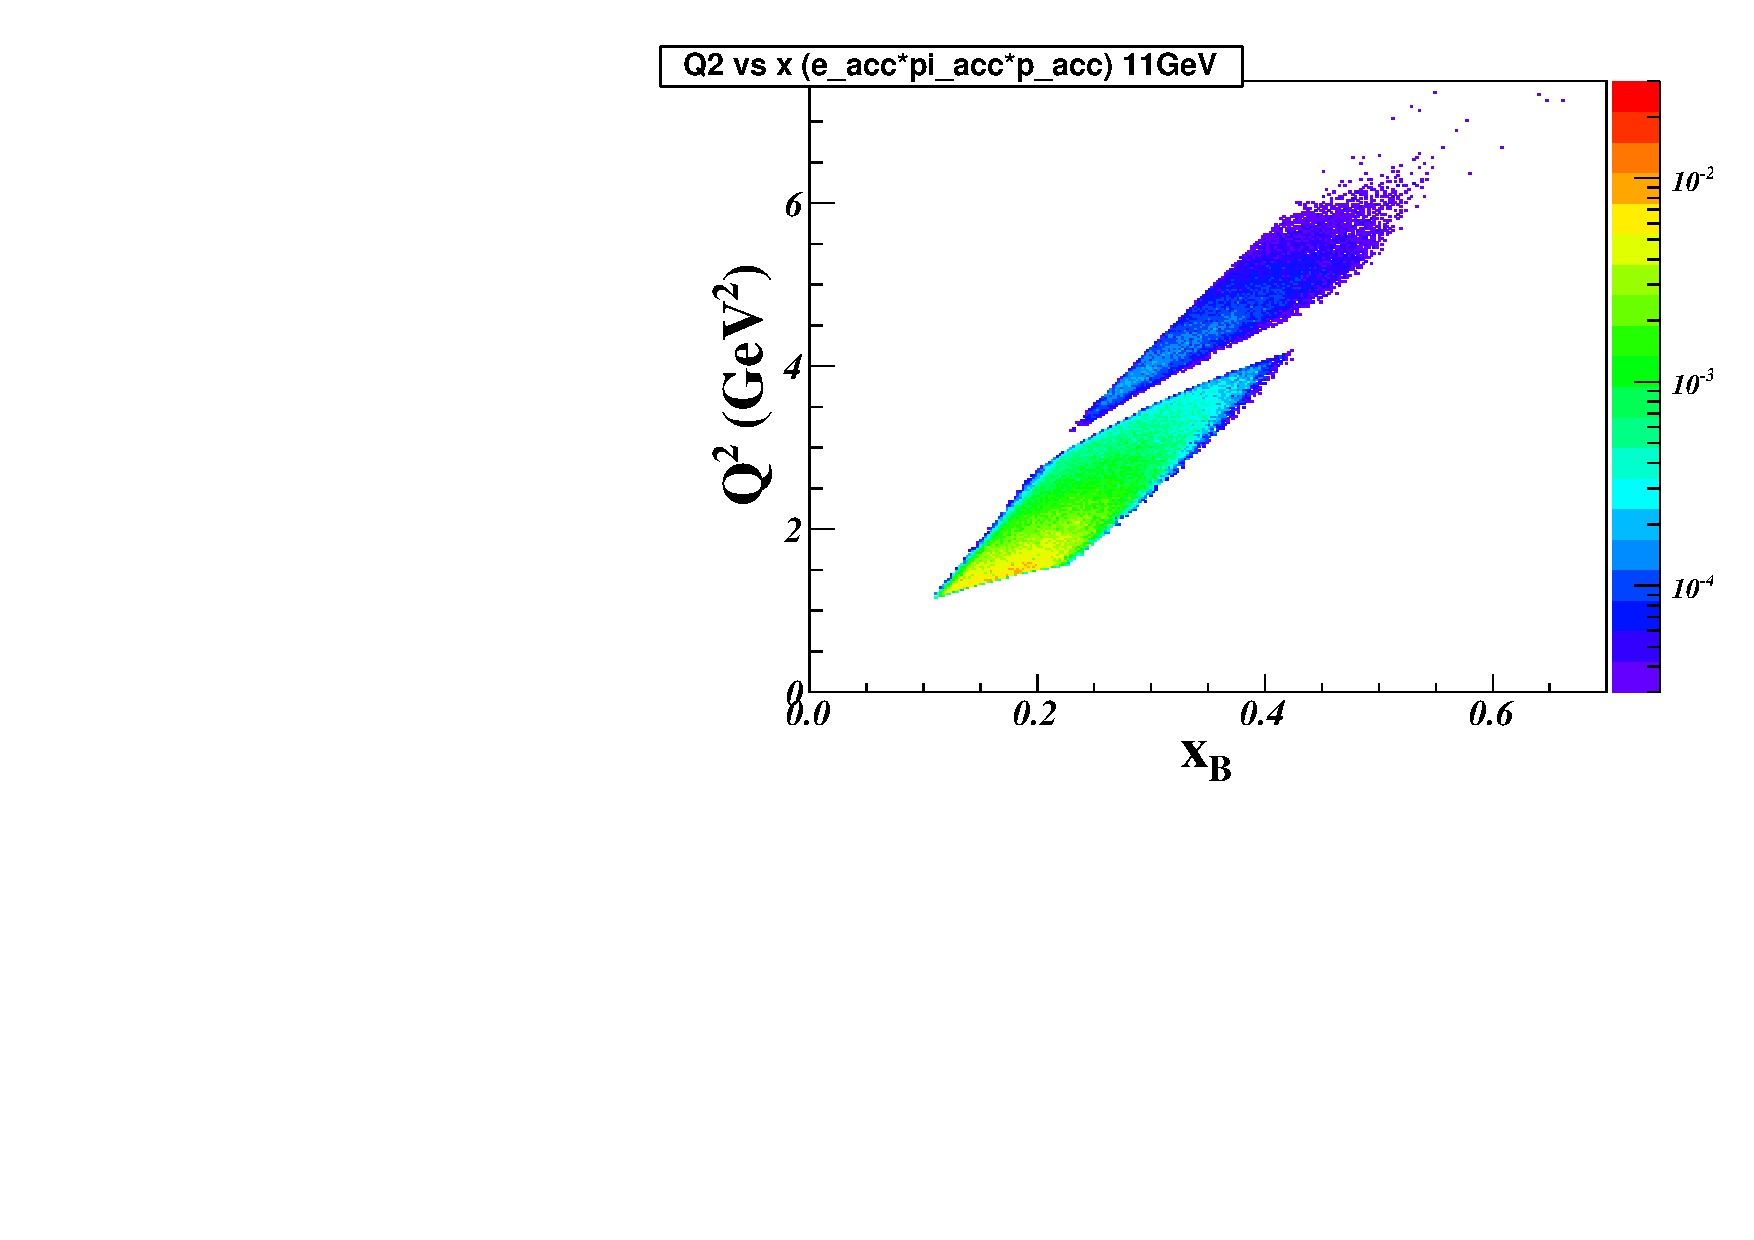
\includegraphics[type=pdf,
        ext=.pdf,read=.pdf,width=0.35\textwidth]{./figures//E11_Q2_x_epip_prd}
    }
     \subfloat[w PRD]{
      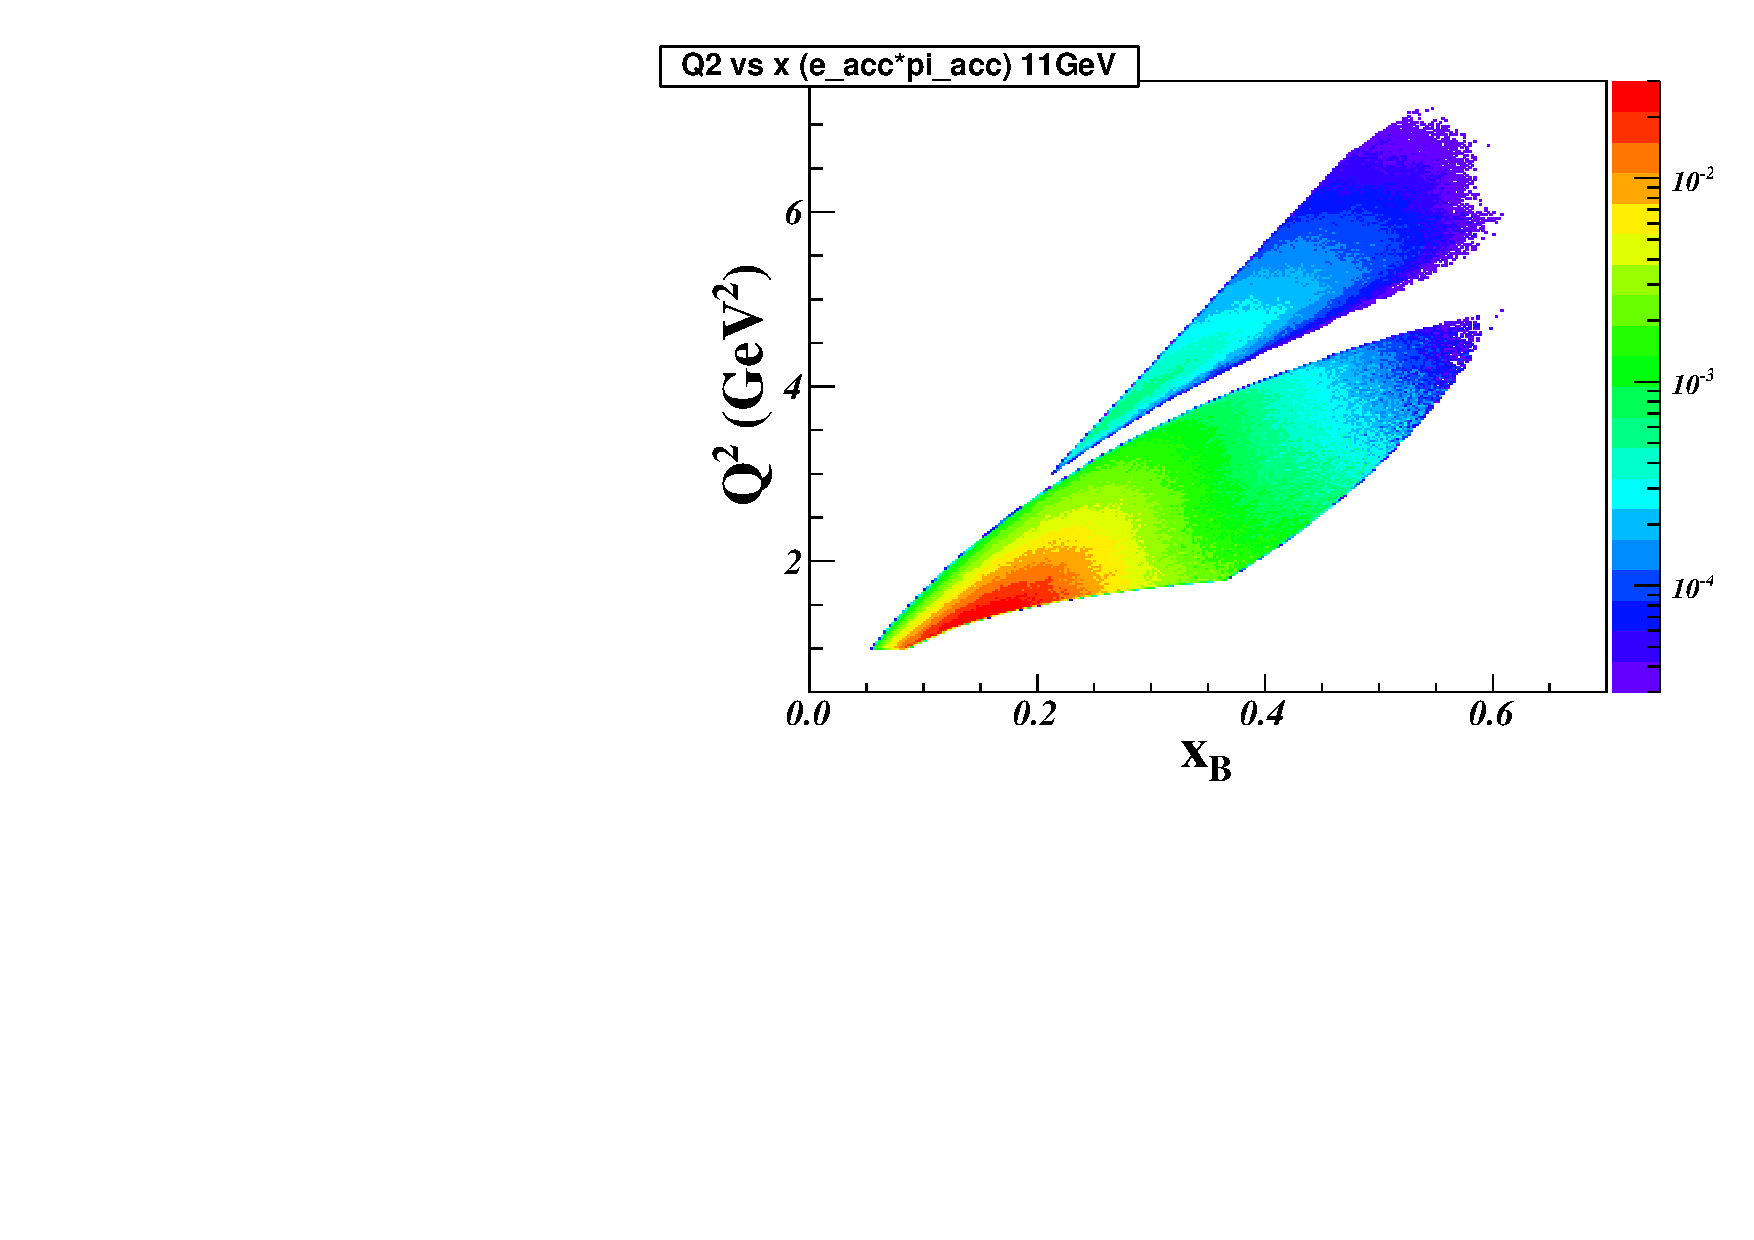
\includegraphics[type=pdf,
        ext=.pdf,read=.pdf,width=0.35\textwidth]{./figures/E11_Q2_x_epip}
    }    
 \caption[The kinematic coverage at different acceptances.]{\footnotesize{The
     kinematic coverage at different acceptances at 11~GeV. The left plot
     shows the coverage with proton detection by existing SoLID
     detectors, while the right  plot
     shows the coverage when detecting all recoil protons with an additional proton detector. Colors correspond to rates (Hz) in log scale.}}
  \label{kin_cor}
  \end{center}
\end{figure}
The kinematic coverage in $Q^{2}$ vs. $x_{B}$ is shown in Fig.~\ref{kin_cor},
where two proton detection cases were given: $(a)$ by using only the SoLID
detectors to detect protons at small angles ($8^{\circ}\sim24^{\circ}$) and
adding a new proton recoil detector to detect the rest of the recoil protons at
larger angle ($24^{\circ}\sim50^{\circ}$), or $(b)$ by only using only the 
SoLID detectors. These distributions were weighted by the DEMP unpolarized
cross sections and the SoLID acceptance obtained from the GEANT4 simulation
with the SoLID-SIDIS configuration. As shown in these plots, the range of
$Q^{2}$ is from 1.0~GeV$^{2}$ to 8.0~GeV$^{2}$, $x_{B}$ goes from 0.1 up to
0.75.

\begin{figure}[!ht]
 \begin{center}
       \subfloat[w/o PRD]{
      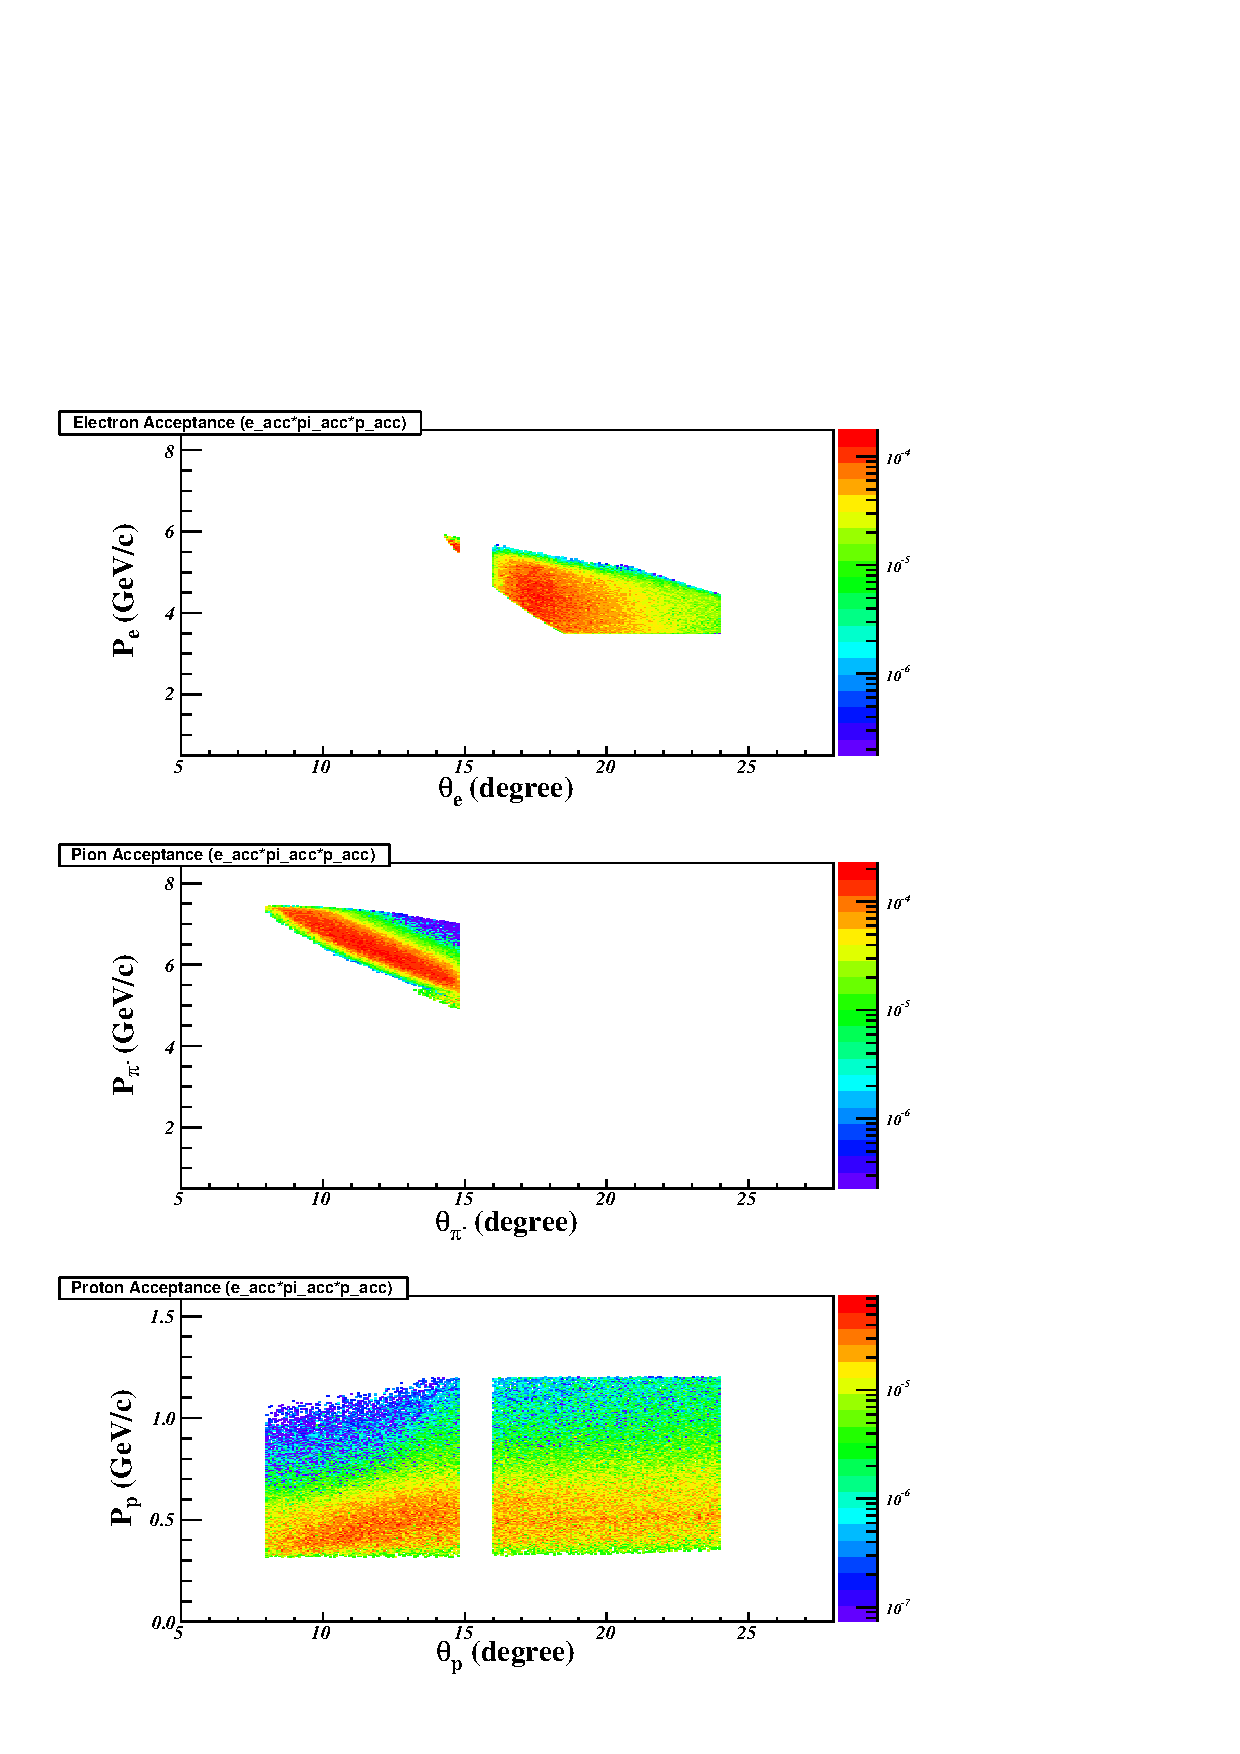
\includegraphics[type=pdf,
        ext=.pdf,read=.pdf,width=0.35\textwidth]{./figures/E11_acc_epip_Q2gt4}
    }
  \subfloat[w/ PRD]{
      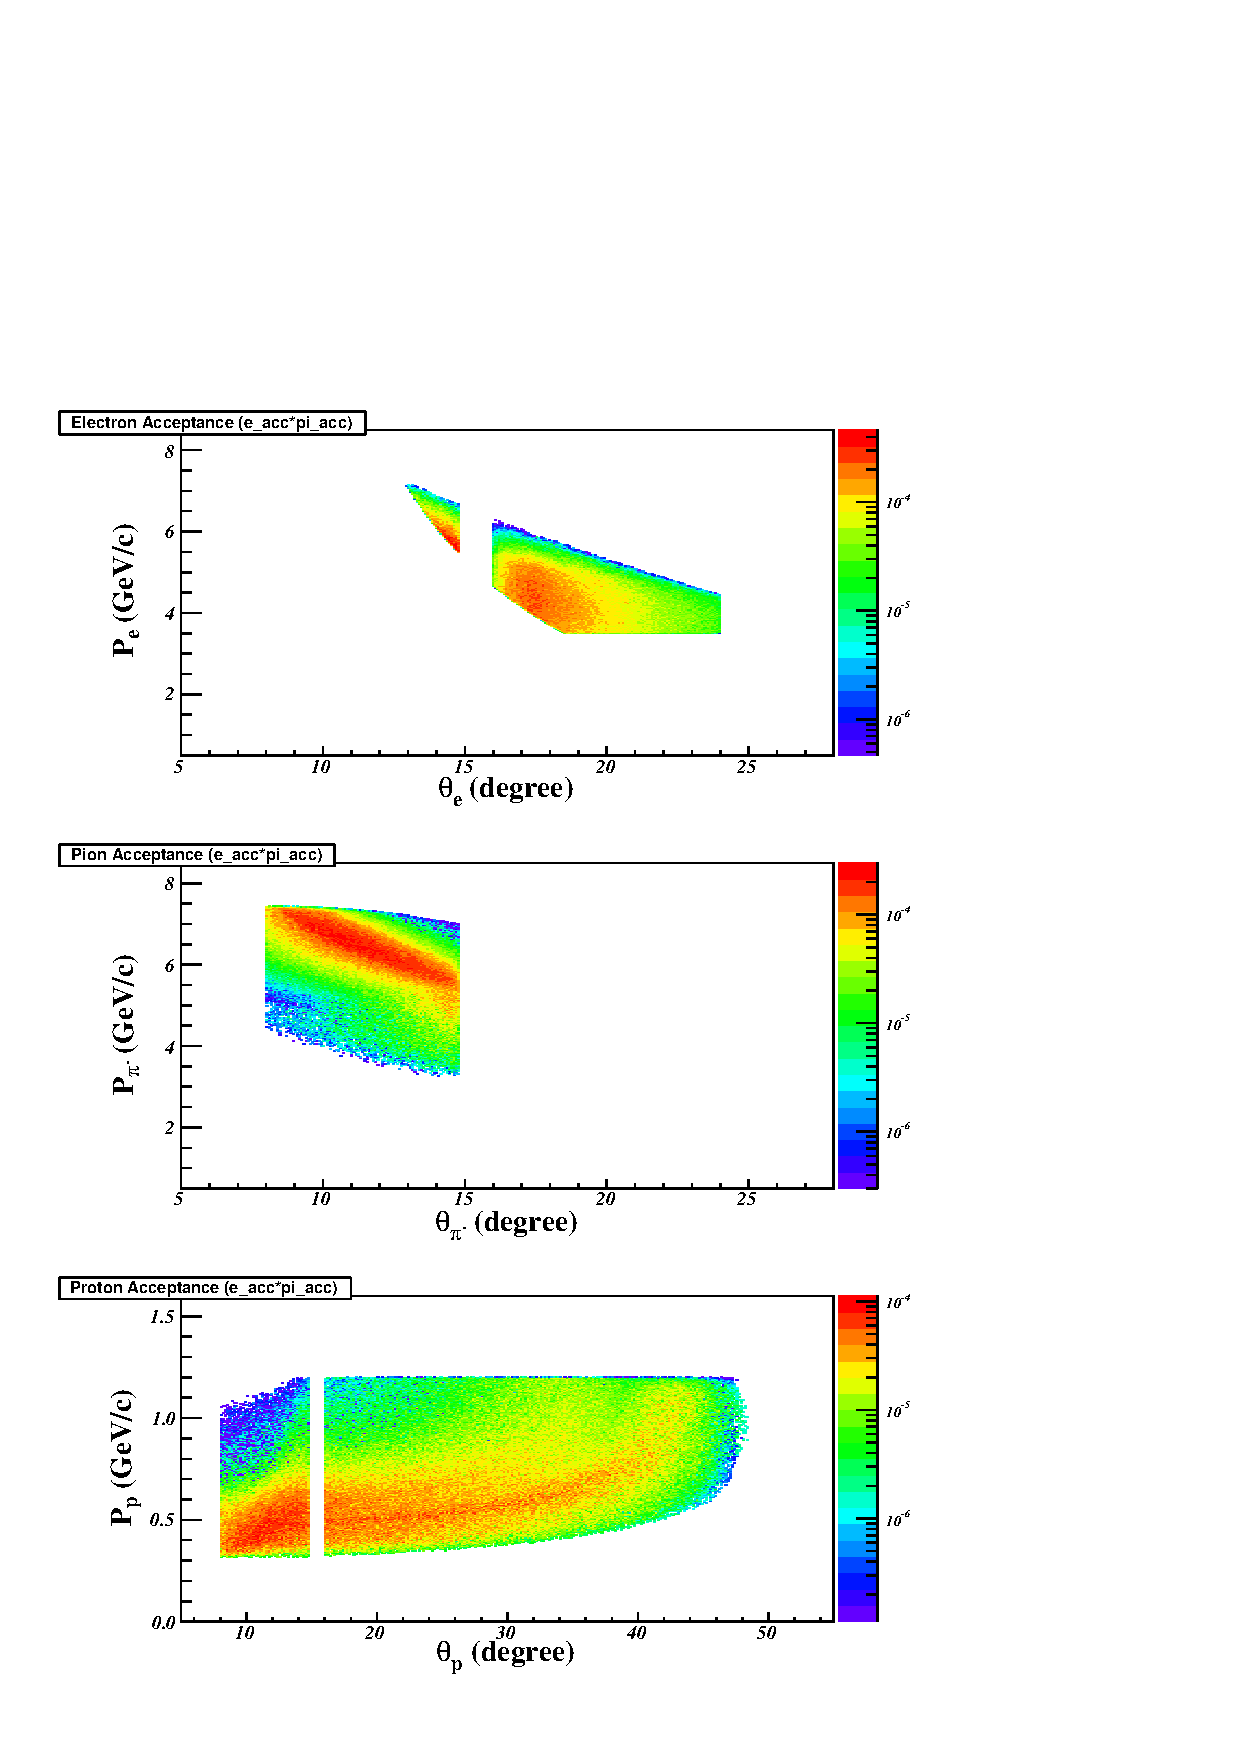
\includegraphics[type=pdf,
        ext=.pdf,read=.pdf,width=0.35\textwidth]{./figures/E11_acc_epi_Q2gt4}
    }  
   \caption[The acceptance of the momenta and scattering angles for electrons,
     $\pi^{-}$ and protons]{\footnotesize{The acceptance of the momenta and
       polar angles w/o or w/ the PRD. In each panel, the top, middle and
       bottom plots are for electrons, $\pi^{-}$ and protons, respectively. A
       cut of $\mathrm{Q^{2}>4~GeV^{2}}$ is applied. Colors correspond to rates
       (Hz) in log scale.}}
  \label{p_theta}
  \end{center}
\end{figure}
Fig.~\ref{p_theta} shows the momentum and angular acceptance of electrons,
$\pi^{-}$ and protons which form the DEMP events and can be detected with the
SoLID detectors and (or) with the new PRD.  A cut of $Q^{2}>$4~GeV$^{2}$
is applied since this is the region of greatest physics itnerest.  The recoil
protons shown in Fig.~\ref{p_theta} have low momenta ranging from 0.3~GeV/c up
to 1.2~GeV/c and their rates are distributed nearly uniformly in scattering
angle.

\subsection{Estimated Rates}
\begin{table}[!ht]
\centering
\begin{tabular}{|c|c|c|}
 \hline
  1$<Q^{2}<$4~GeV$^{2}$ & $Q^{2}>$4~GeV$^{2}$ & Total\\
 \hline
\multicolumn{3}{|c|}{DEMP: $\vec{n}(e,e'\pi^{-}p)$ Triple-Coincidence (Hz)}\\
 \hline
 23.91 (6.21)   &  0.59 (0.28) & 24.50 (6.49)   \\
 \hline
\multicolumn{3}{|c|}{SIDIS: $\vec{n}(e,e'\pi^{-})X$ Double-Coincidence (Hz)}\\
 \hline
        1388.85 & 35.77        & 1424.62   \\
 \hline
\end{tabular}
\caption[Triple-Coincidence rates for
  neutron-DEMP]{\footnotesize{Triple-Coincidence rates for DEMP events compared
    with the SIDIS rates. Numbers in brackets are the DEMP rates with only
    detecting protons using only the SoLID detectors. The online production
    trigger will be the SIDIS double-coincidence trigger of which rates are
    also given.}}
\label{rate_table}
\end{table} 
Table~\ref{rate_table} lists the triple-coincidence rate of the DEMP
events. The rates were calculated with the simulated events weighted by the
target luminosity, the SoLID acceptances and unpolarized cross sections. The
rates are not corrected by the beam and target polarization, target dilution
and so on. The total integrated physics rate is estimated to be around 25~Hz at
11~GeV, or 0.59 Hz at $Q^{2}>$4~GeV$^{2}$. If only using only the 
SoLID detectors to detect protons, the rate drops to 0.28 Hz at
$Q^{2}>$4~GeV$^{2}$.  For comparison, the table also gives the SIDIS rate
which will be the online production trigger rates and is the main background of
the DEMP events.

\subsection{Asymmetry Projections}
\begin{figure}[!ht]
 \begin{center}
       \subfloat[w/o PRD]{
      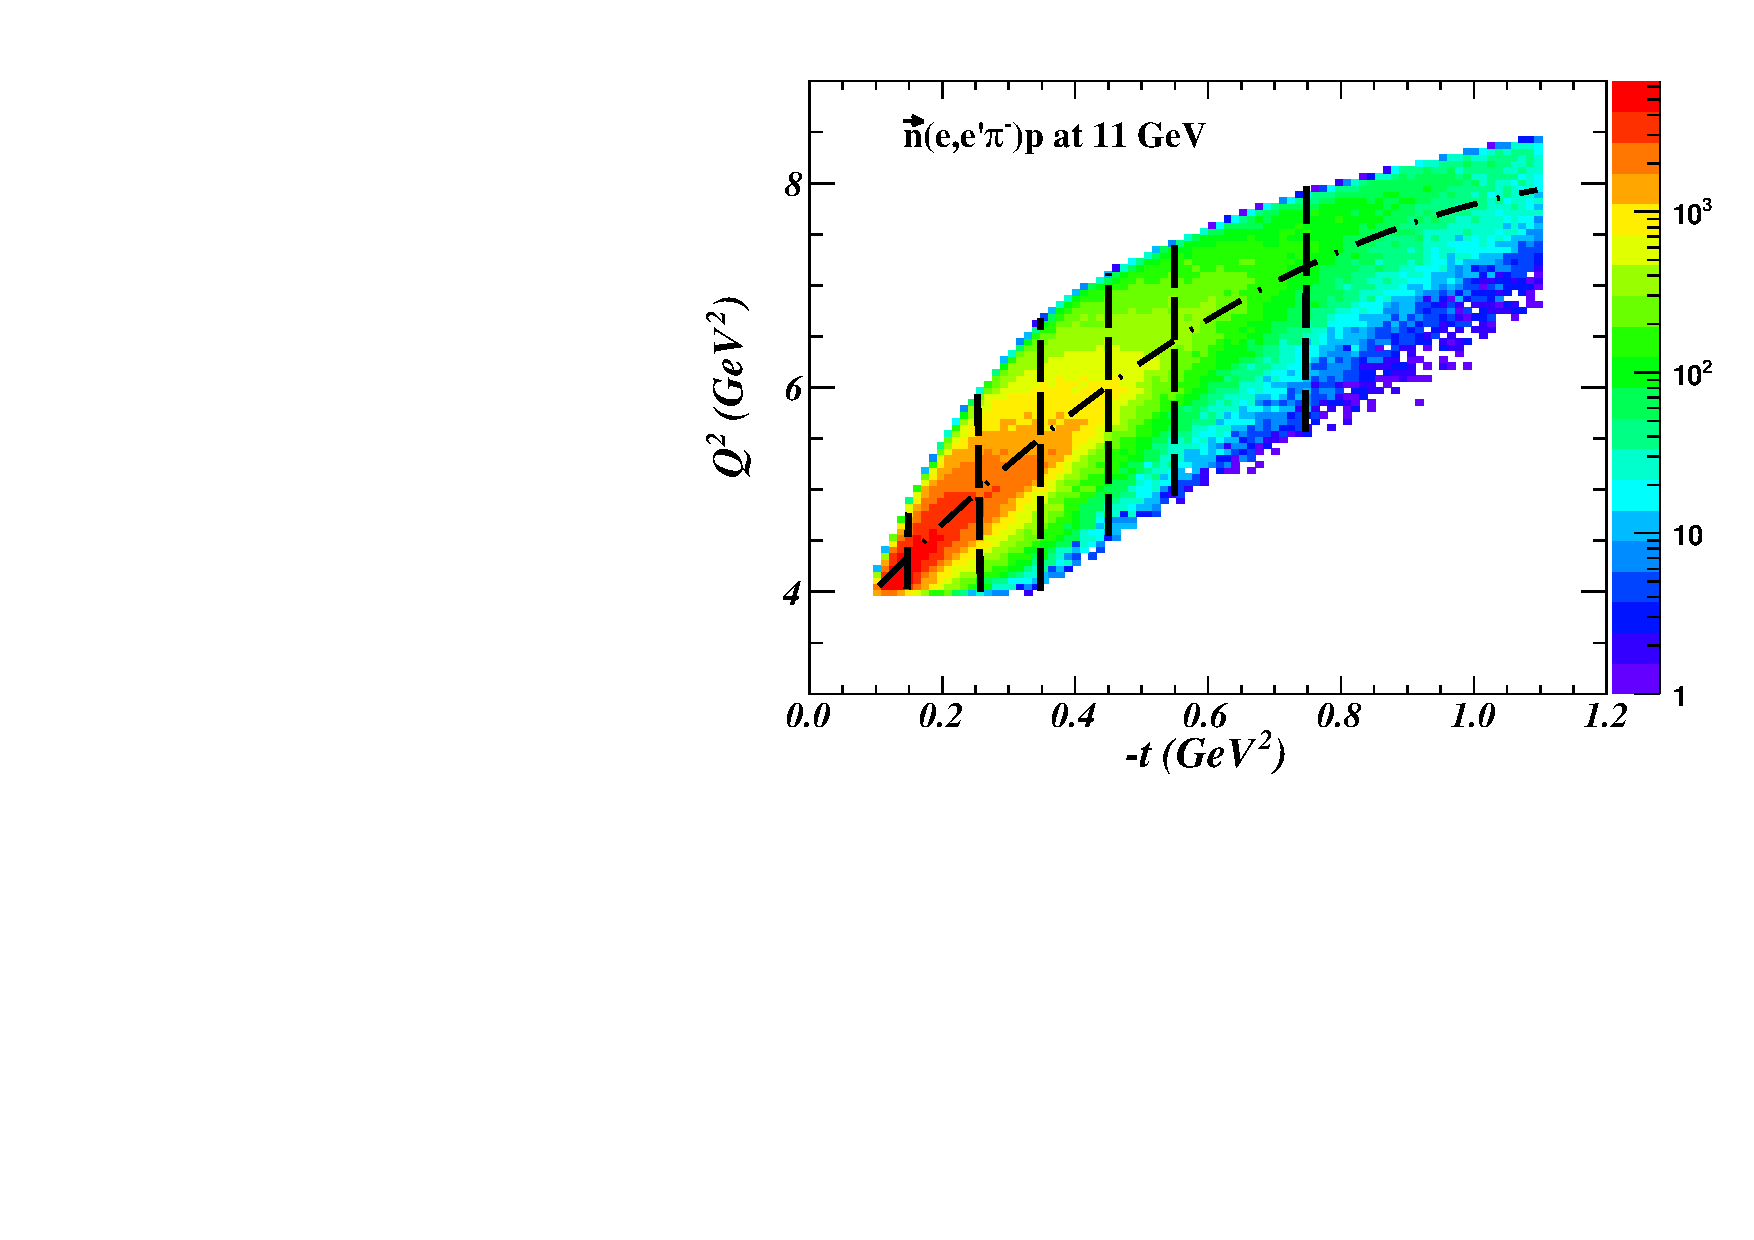
\includegraphics[type=pdf,
        ext=.pdf,read=.pdf,width=0.5\textwidth]{./figures/E11_Q2_t_bin_New} }
        \subfloat[w/ PRD]{
      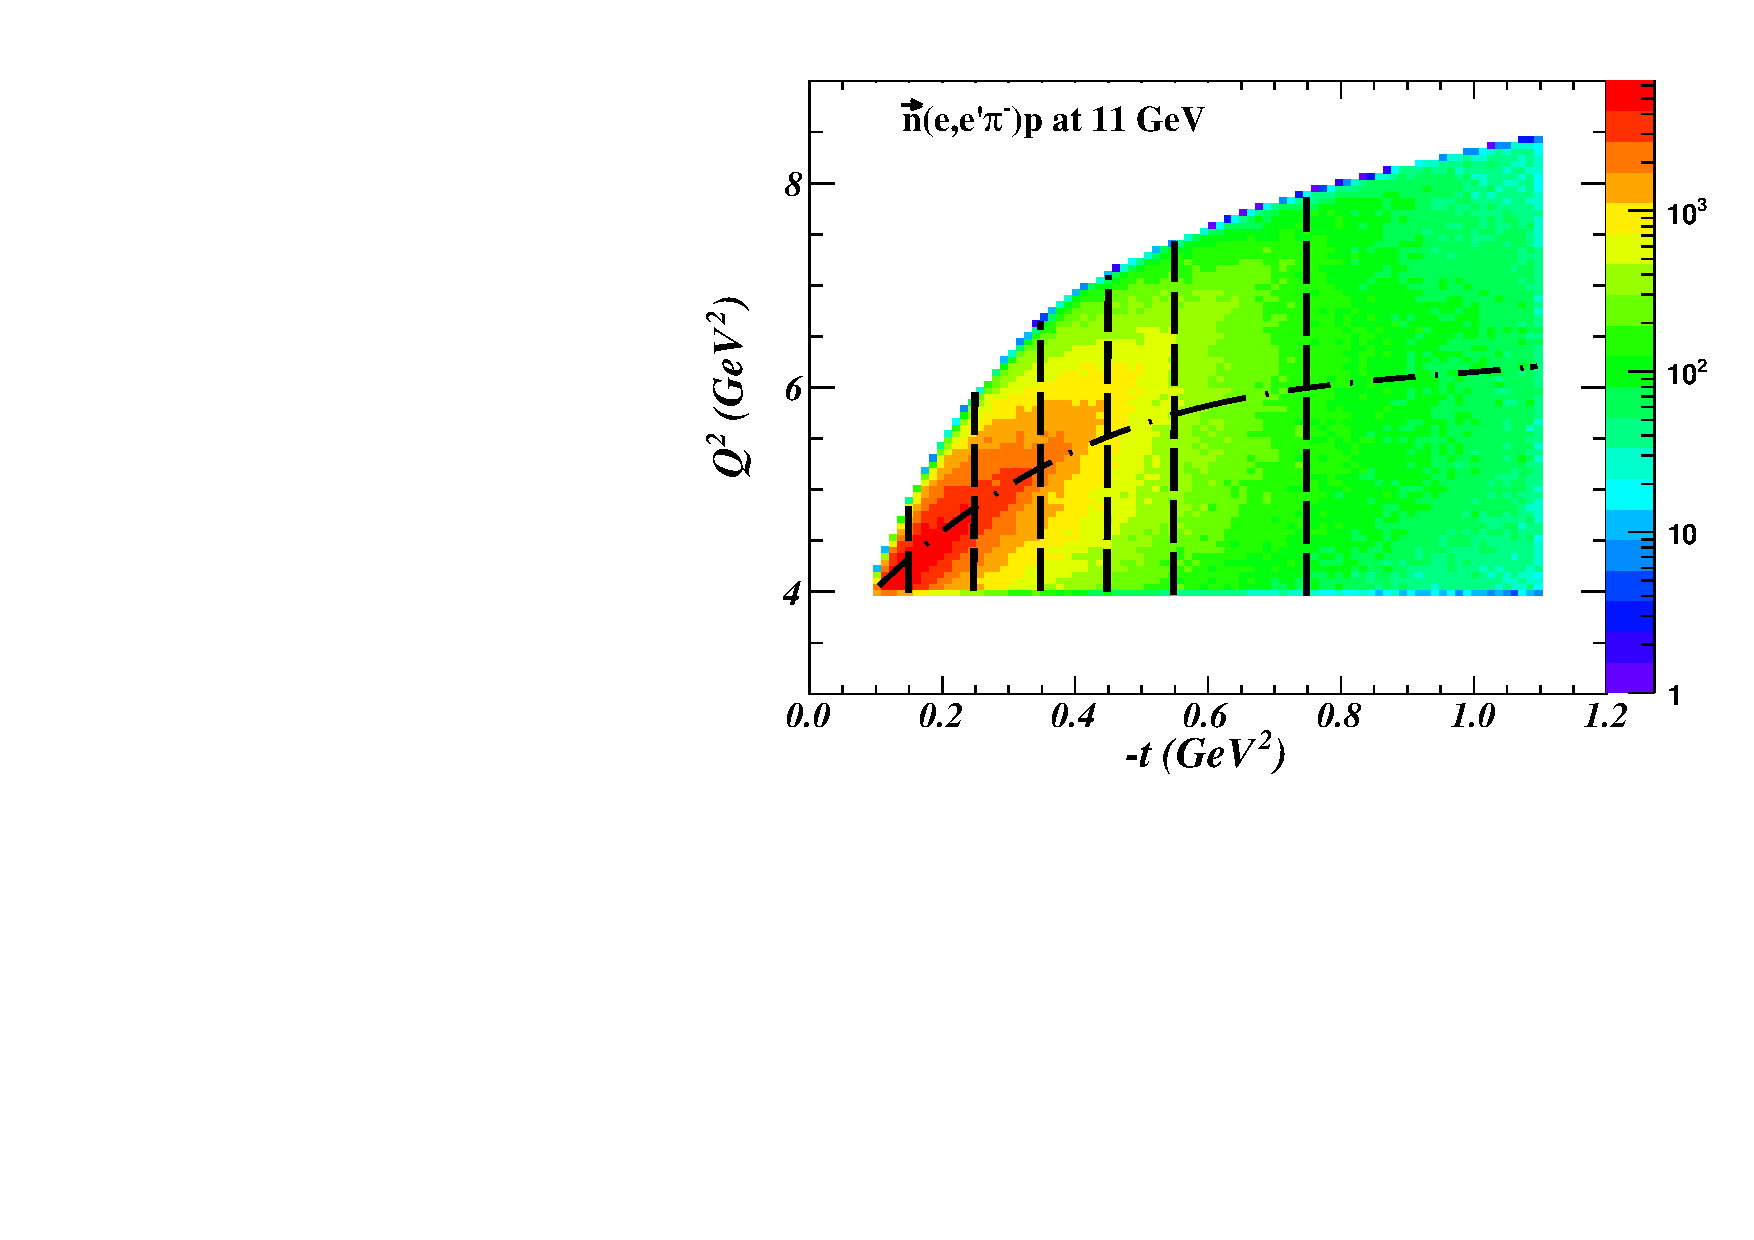
\includegraphics[type=pdf,
        ext=.pdf,read=.pdf,width=0.5\textwidth]{./figures/E11_Q2_t_bin_prd_New} }
   \caption[$Q^{2}$ vs. $-t$]{\footnotesize{$Q^{2}$ vs. $-t$ where the black
       dash lines specify the boundaries of 7 $-t$ bins and the black dash-dot lines indicate the additional 2 $Q^{2}$ bins. 
       The color panel indicates the raw counts with 48 days of beam time at 11~GeV.}}
  \label{Q2_t_bin}
  \end{center}
\end{figure}
The proposed experiment will run in parallel with E12-10-006 which has already
been approved to run 48 days at $E_{0}$=11~GeV.  As shown in
Fig.~\ref{Q2_t_bin}, We defined 7 $-t$ bins of which the the boundaries are
defined by the array:
 \begin{equation}
   -t[8] = [0.0, 0.15, 0.25, 0.35, 0.45, 0.55, 0.75, 1.10]~~~~(in~\mathrm{GeV^{2}})
 \end{equation}
The number of events ($N_{i}$) in the $i$th bin is calculated from the total
simulated events after applying cuts on important kinematic variables,
e.g. $Q^{2}>$4~GeV$^{2}$, $W>$2~GeV, 0.55$<\epsilon<$0.75 and
$-t_{min}<-t<-t_{max}$. As shown in Eq.~\ref{ncount}, each event surviving the
cuts is then weighted by the unpolarized cross section, together with the
acceptance of the electron, pion and proton. $N_{i}$ is further corrected by
the phase-space factor ($PSF$) defined in the event generator, the total number
of randomly generated events ($N_{gen}$), beam-time ($T$), the target
luminosity ($L=10^{36}$~cm$^{-2}$s$^{-1}$), and the overall detector efficiency 
($\epsilon_{eff}$):
 \begin{equation}
     N_{i} = \bigl(\sum_{j\in i-bin} \sigma_{j}\cdot A^{e}_{j} \cdot
     A^{\pi^{-}}_{j} \cdot A^{p}_{j}\bigr) \cdot (PSF/N_{gen}) \cdot T \cdot L \cdot
     \epsilon_{eff},
     \label{ncount}
 \end{equation}
where $j$ is the $j$th event in the $i$th bin, $\sigma_{j}$ is the cross
section of the $j$th event. $A^{e(\pi^{-},p)}_{j}$ is the acceptance weight of the
electron (pion, proton) in this event. The detector efficiency,
$\epsilon_{eff}$, is approximately fixed at 85\% which was used in SIDIS
proposals. $N_{i}$ corresponds to the raw experimental count of electrons
scattering on neutrons in $\mathrm{^{3}He}$ before taking into account the
target polarization ($P\sim60\%$), the effective polarization of neutrons
($\eta_{n}\sim0.865$), and the dilution effect from other reaction channels
when electrons scattering on $\mathrm{^{3}He}$ ($f \sim 0.9$). 

In addition, we further divide each $-t$-bin into two $Q^{2}$ bins with similar statistics. 
By doing that we are able to examine the $Q^{2}$-dependence of the asymmetries, 
and also check the model dependence of other corrections that are directly related to the values of $Q^{2}$.

The statistical error of the target single spin asymmetry ($A_{UT}$) in each bin can be given
as:
  \begin{equation}
    \delta A_{UT} = \frac{1}{P\cdot\eta_{n}\cdot f} \sqrt{\frac{1-(P\cdot
        <A_{UT}>)^{2}}{N^{+}_{i}+N^{-}_{i}}},
    \label{stat_err}
 \end{equation}
where $N^{+(-)}_{i}$ is the number of counts in each bin when the target
polarization is up (down), and we easily have $N_{i}=N^{+}_{i}+N^{-}_{i}$;
$<A_{UT}>$ is the average asymmetry in the bin, and experimentally, it can be
extracted as following:
\begin{equation}
   <A_{UT}> = \frac{1}{P\cdot\eta_{n}\cdot f} \frac{N^{+}-N^{-}}{N^{+}+N^{-}}.
   \label{asym_exp}
\end{equation}
In this projection study, $A_{UT}$ is predicted with a phenomenological model,
as discussed in Appendix-A. Because of not performing a L/T separation in this
experiment, the asymmetry should be corrected by another dilution factor which
is defined as:
\begin{equation}
  f_{L/T} =\frac{\epsilon\sigma_{L} }{\sigma_{T}+\epsilon\cdot\sigma_{L} },
\end{equation} 
where $\epsilon=(1+\frac{2\nu^{2}}{Q^{2}}\tan^{2}(\theta))^{-1}$. Additional dilution
due to $\sigma_{TT}$ is assumed to be small.  A factor of $-1$ is also applied after comparing Eq.~\ref{eqn:asy} and Eq.~\ref{eqn:sigtarg}. Hence, $A_{UT} = -f_{L/T}\cdot A_{L}^{\perp,model}$.

\begin{figure}[!ht]
 \begin{center}
         \subfloat[w/o PRD]{
               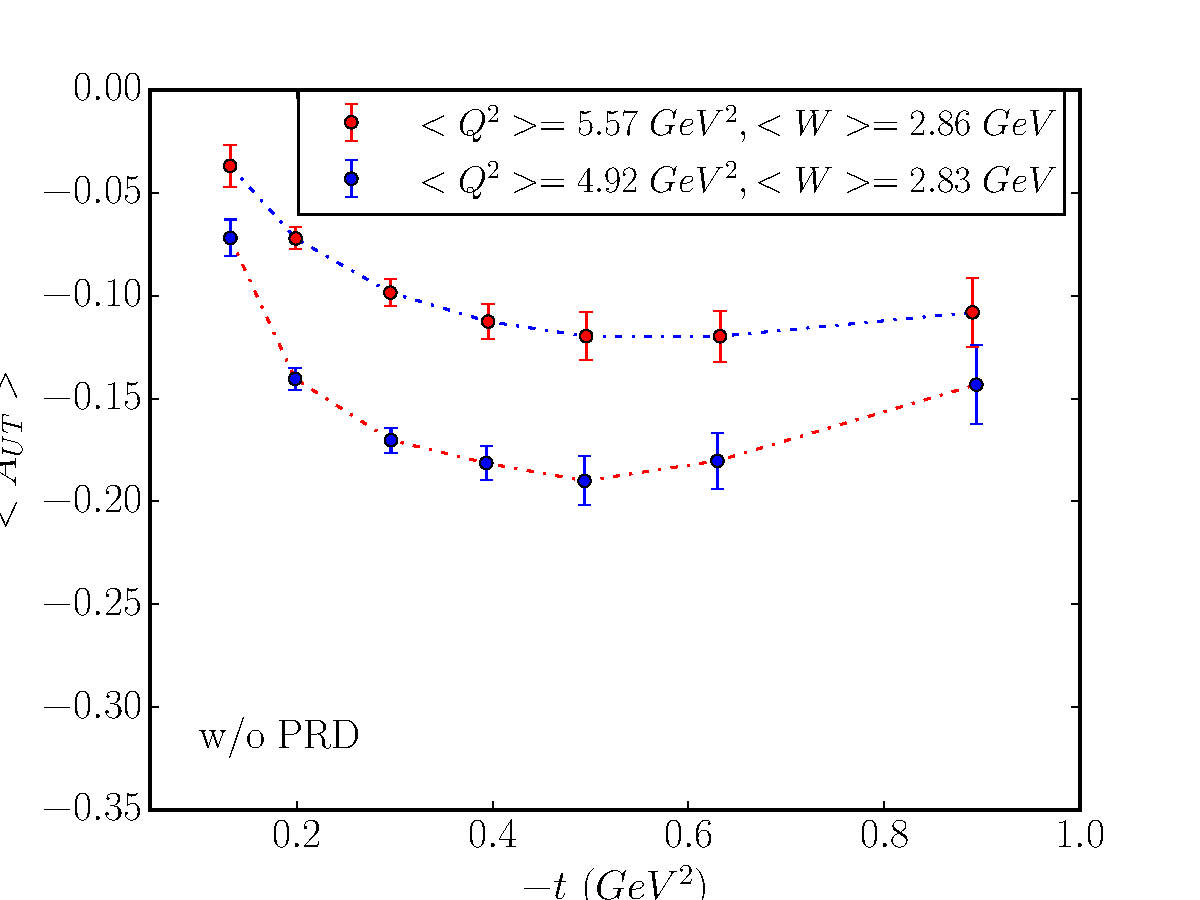
\includegraphics[type=pdf,
        ext=.pdf,read=.pdf,width=0.45\textwidth]{./figures/bin_asym_t_new} }
            \subfloat[w/ PRD]{
      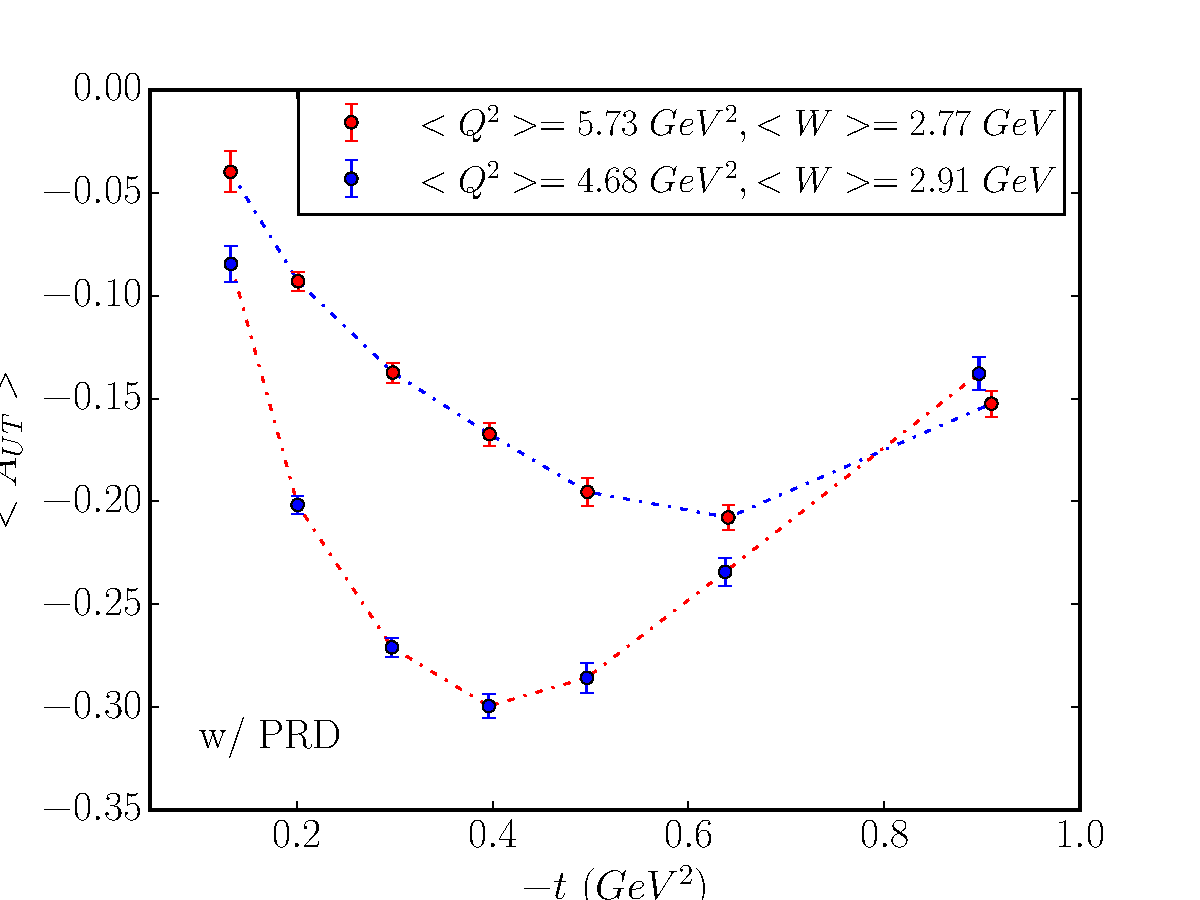
\includegraphics[type=pdf,
        ext=.pdf,read=.pdf,width=0.45\textwidth]{./figures/bin_asym_t_prd_new} }
      \caption{\footnotesize{Projection of target sing spin asymmetry
          ($A_{UT}$) as a function of $-t$ for DEMP with transversely polarized
          $\mathrm{^{3}He}$ at $E_{0}$=11~GeV (directly compared with Fig.~\ref{fig:hermes_aut}). 
          The data in each $-t$ bin are further divided into two $Q^{2}$ bins with similar statistics. 
          The error bars are the projected
          statistical uncertainties defined in Eq.~\ref{stat_err}. The
          asymmetry value in each bin is predicted with the model given in Appendix-A and is diluted due to not separating the L/T
          contributions. The left plot shows the projection w/o a new proton
          recoil detector, while the right plot shows a better projected result
          with a new detector in addition. One can see the average asymmetries are also
          changed between two configurations and it is because the asymmetry
          strongly depends on $Q^{2}$ which changes w/ or w/o the PRD.}}
  \label{asym_t}
  \end{center}
\end{figure}
Fig.~\ref{asym_t} shows the distribution of $A_{UT}$ vs. $-t$ with projected
statistical errors discussed above. Compared with the existing HERMES results
(Fig.~\ref{fig:hermes_aut}), the new measurement could provide more precision
data to be directly compared with theoretical predictions. Extra binning on $Q^{2}$ enables us to 
study the $Q^{2}$-dependence of asymmetries as well as to constraint some corrections during the asymmetry extraction. 
The detailed information of each bin is listed in Table~\ref{asym_bin_table}.

%	\begin{table}[!ht]
%	\centering
%	  \small
%	\begin{tabular}{|c|c|c|c|c|c|c|c|}
%	  \hline
%	w/o PRD   &  Bin\#1 & Bin\#2 & Bin\#3 & Bin\#4 & Bin\#5 & Bin\#6 & Bin\#7 \\
%	\hline 
%	    $<-t>$                &  0.13 & 0.20   & 0.30   & 0.39   & 0.49   & 0.63   & 0.89  \\
%	   $<Q^{2}>$          & 4.22  & 4.67   & 5.23   & 5.78   & 6.26   & 6.81  & 7.59  \\
%	   $<A_{UT}>$        &$-5.67\times 10^{-2}$   & $-1.07\times 10^{-1}$   & $-1.36\times 10^{-1}$    & $-1.47\times 10^{-1}$    & $-1.54\times 10^{-1}$    & $-1.47\times 10^{-1}$   & $-1.23\times 10^{-1}$   \\
%	   $\delta A_{UT}$  &  $6.76\times 10^{-3}$   & $3.73\times 10^{-3}$    &   $4.42\times 10^{-3}$  &  $5.92\times 10^{-3}$   &  $8.30\times 10^{-3}$   &   $9.15\times 10^{-3}$ &   $1.26\times 10^{-2}$ \\
%	   $N$                     & $6.07\times 10^{4}$   &$1.99\times 10^{5}$   & $1.41\times 10^{5}$   &  $7.87\times 10^{4}$  & $4.00\times 10^{4}$  &  $3.29\times 10^{4}$ &$1.75\times 10^{4}$  \\
%	 \hline
%			\multicolumn{3}{c}{ } \\
%   	\hline 
%	w/ PRD   &  Bin\#1 & Bin\#2 & Bin\#3 & Bin\#4 & Bin\#5 & Bin\#6 & Bin\#7 \\
%	 \hline
%	  $<-t>$                &  0.13 & 0.20   & 0.30   & 0.40   & 0.50   & 0.64   & 0.90  \\
%	   $<Q^{2}>$          & 4.22  & 4.59   & 5.02   & 5.38   & 5.64   & 5.90  & 6.27  \\
%	   $<A_{UT}>$        &$-6.53\times 10^{-2}$   & $-1.51\times 10^{-1}$   & $-2.06\times 10^{-1}$    & $-2.30\times 10^{-1}$    & $-2.38\times 10^{-1}$    & $-2.20\times 10^{-1}$   & $-1.47\times 10^{-1}$   \\
%	   $\delta A_{UT}$  &  $6.50\times 10^{-3}$   & $3.15\times 10^{-3}$    &   $3.36\times 10^{-3}$  &  $4.05\times 10^{-3}$   &  $5.02\times 10^{-3}$   &   $4.64\times 10^{-3}$ &   $4.95\times 10^{-3}$ \\
%	   $N$                     & $6.55\times 10^{4}$   &$2.78\times 10^{5}$   & $2.43\times 10^{5}$   &  $1.66\times 10^{5}$  & $1.08\times 10^{5}$  &  $1.27\times 10^{5}$ &$1.13\times 10^{5}$  \\
%	 \hline
%	\end{tabular}
%	\caption[Detailed information of projected bins]{\footnotesize{Detailed information of projected bins from the new DEMP measurements with SoLID, while $<Q^{2}>$ and $<-t>$ are in the unit of $GeV^{2}$. The top (bottom) table is with respect to the case of proton detection w/o (w/) a new PRD.}}
%	\label{asym_bin_table}
%\end{table} 


	\begin{table}[!ht]
	\centering
	  \small
	\begin{tabular}{|c|c|c|c|c|c|c|c|}
	 \multicolumn{8}{c}{ (a) w/o PRD} \\
	  \hline
	      &  t-bin\#1 & t-bin\#2 & t-bin\#3 & t-bin\#4 & t-bin\#5 & t-bin\#6 & t-bin\#7 \\
	\hline 
	    $<-t>$                &  0.13 & 0.20   & 0.30   & 0.40   & 0.50   & 0.63   & 0.89  \\
	      \hline
   	  \multicolumn{8}{|c|}{$Q^{2}$ bin-set\#1 } \\
   	    \hline
   	   $<Q^{2}>$          & 4.12  & 4.44   & 4.92   & 5.40   & 5.87   & 6.43  & 7.31  \\
   	   $<\sigma_{L}/\sigma_{T}>$ & 6.17 & 5.19 & 4.24 & 3.59 & 3.00 & 2.23 & 1.08 \\
   	   $<f_{L/T}>$        & 0.79 & 0.77 & 0.74 & 0.71 & 0.67 & 0.60 & 0.41 \\
	   $<A_{UT}>$        &$-7.20\times 10^{-2}$   & $-1.40\times 10^{-1}$   & $-1.70\times 10^{-2}$    & $-1.81\times 10^{-1}$    & $-1.90\times 10^{-1}$    & $-1.80\times 10^{-1}$   & $-1.19\times 10^{-1}$   \\
	   $\delta A_{UT}$  &  $8.98\times 10^{-3}$   & $5.20\times 10^{-3}$    &   $6.10\times 10^{-3}$  &  $8.30\times 10^{-3}$    &  $1.19\times 10^{-2}$   &   $1.36\times 10^{-2}$ &   $1.91\times 10^{-2}$ \\
	   $N$                     & $3.44\times 10^{4}$   &$1.02\times 10^{5}$   & $7.38\times 10^{4}$   &  $3.98\times 10^{4}$  & $1.93\times 10^{4}$  &  $1.48\times 10^{4}$ &$7.55\times 10^{3}$  \\
  \hline
   	  \multicolumn{8}{|c|}{$Q^{2}$ bin-set\#2 } \\
  \hline 
   	   $<Q^{2}>$          & 4.36  & 4.91   & 5.58   & 6.16   & 6.62   & 7.13  & 7.80  \\
	   $<\sigma_{L}/\sigma_{T}>$ & 6.74 & 6.32 & 5.76 & 5.12 & 4.29 & 3.14 & 1.66 \\
   	   $<f_{L/T}>$        & 0.80 & 0.79 & 0.78 & 0.76 & 0.73 & 0.66 & 0.51 \\
	   $<A_{UT}>$        &$-3.69\times 10^{-2}$   & $-7.22\times 10^{-2}$   & $-9.85\times 10^{-2}$    & $-1.13\times 10^{-1}$    & $-1.20\times 10^{-1}$    & $-1.20\times 10^{-1}$   & $-1.08\times 10^{-1}$   \\
	   $\delta A_{UT}$  &  $1.03\times 10^{-2}$   & $5.35\times 10^{-3}$    &   $6.42\times 10^{-3}$  &  $8.44\times 10^{-3}$   &  $1.16\times 10^{-2}$   &   $1.24\times 10^{-2}$ &   $1.67\times 10^{-2}$ \\
	   $N$                     & $2.63\times 10^{4}$   &$9.70\times 10^{4}$   & $6.72\times 10^{4}$   &  $3.89\times 10^{4}$  & $2.07\times 10^{4}$  &  $1.81\times 10^{4}$ &$9.94\times 10^{3}$  \\
     \hline
	  \multicolumn{8}{c}{} \\
	  \multicolumn{8}{c}{ (b) w/ PRD} \\
	   \hline
	     &  t-bin\#1 & t-bin\#2 & t-bin\#3 & t-bin\#4 & t-bin\#5 & t-bin\#6 & t-bin\#7 \\
     	\hline 
		    $<-t>$                &  0.13 & 0.20   & 0.30   & 0.40   & 0.50   & 0.64   & 0.90  \\
	    \hline
   	   \multicolumn{8}{|c|}{$Q^{2}$ bin-set\#1 } \\
   	    \hline
   	   $<Q^{2}>$          & 4.11  & 4.35   & 4.65   & 4.84   & 4.97   & 5.08  & 5.18  \\
   	   $<\sigma_{L}/\sigma_{T}>$ & 6.12 & 4.88 & 3.60 & 2.60 & 1.86 & 1.18 & 0.52 \\
   	   $<f_{L/T}>$        & 0.79 & 0.76 & 0.70 & 0.63 & 0.55 & 0.43 & 0.25 \\
	   $<A_{UT}>$        &$-8.46\times 10^{-2}$   & $-2.02\times 10^{-1}$   & $-2.71\times 10^{-2}$    & $-2.99\times 10^{-1}$    & $-2.86\times 10^{-1}$    & $-2.34\times 10^{-1}$   & $-1.38\times 10^{-1}$   \\
	   $\delta A_{UT}$  &  $8.62\times 10^{-3}$   & $4.29\times 10^{-3}$    &   $4.66\times 10^{-3}$  &  $5.85\times 10^{-3}$    &  $7.32times 10^{-3}$   &   $6.86\times 10^{-3}$ &   $7.91\times 10^{-3}$ \\
	   $N$                     & $3.73\times 10^{4}$   &$1.49\times 10^{5}$   & $1.25\times 10^{5}$   &  $7.85\times 10^{4}$  & $5.04\times 10^{4}$  &  $5.78\times 10^{4}$ &$4.41\times 10^{4}$  \\
  \hline
     	   \multicolumn{8}{|c|}{$Q^{2}$ bin-set\#2 } \\
  \hline 
   	   $<Q^{2}>$          & 4.35  & 4.86   & 5.42   & 5.87   & 6.22   & 6.60  & 6.97  \\
	   $<\sigma_{L}/\sigma_{T}>$ & 6.71 & 6.13 & 5.29 & 4.42 & 3.51 & 2.31 & 0.91 \\
   	   $<f_{L/T}>$        & 0.80 & 0.79 & 0.77 & 0.74 & 0.69 & 0.59 & 0.35 \\
	   $<A_{UT}>$        &$-3.98\times 10^{-2}$   & $-9.30\times 10^{-2}$   & $-1.37\times 10^{-1}$    & $-1.67\times 10^{-1}$    & $-1.95\times 10^{-1}$    & $-2.08\times 10^{-1}$   & $-1.52\times 10^{-1}$   \\
	   $\delta A_{UT}$  &  $9.92\times 10^{-3}$   & $4.63\times 10^{-3}$    &   $4.83\times 10^{-3}$  &  $5.61\times 10^{-3}$   &  $6.91\times 10^{-3}$   &   $6.29\times 10^{-3}$ &   $6.35\times 10^{-3}$ \\
	   $N$                     & $2.82\times 10^{4}$   &$1.29\times 10^{5}$   & $1.18\times 10^{5}$   &  $8.75\times 10^{4}$  & $5.74\times 10^{4}$  &  $6.90\times 10^{4}$ &$6.84\times 10^{4}$  \\
 \hline
	\end{tabular}
	\caption[Detailed information of projected bins]{\footnotesize{Detailed information of projected bins from the new DEMP measurements with SoLID, while $<Q^{2}>$ and $<-t>$ are in the unit of $GeV^{2}$. The top (bottom) table is with respect to the case of proton detection w/o (w/) a new PRD. The data are divided into 14 $-t$ bins in both $-t$ (7 bins) and $Q^{2}$ (2 bins). }}
	\label{asym_bin_table}
\end{table} 


\section{Missing Mass and Background}
In the DEMP with a neutron, two charged particles, $\pi^{-}$ and $p$, can be cleanly measured by the detector system. 
Moreover, the stuck proton will also be measured. 
Hence, contamination from other reactions, including DEMP with other two protons in $^{3}He$, can be greatly eliminated.
The dominant background of the DEMP measurement comes from the SIDIS reactions
of electrons scattering on the neutron and two protons in $\mathrm{^{3}He}$. In
addition to detecting the recoil protons, which should largely suppress most of
background, we will also rely on reconstructing the neutron missing mass
spectrum to ensure the exclusivity of the DEMP events. In SIDIS, however, the
final states include the scattered electron, the hadrons ($\pi^{\pm}$,
$K^{\pm}$ etc.), as well as the undetected target fragments which could contain
protons. Hence, the SIDIS events will possibly leak into the DEMP missing mass
spectrum.

We studied the contamination of the SIDIS events in the DEMP missing momentum
and mass spectra. The SIDIS reactions, $p(e,e'\pi^{-})X$ and $n(e,e'\pi^{-})X$,
were simulated with the same generator used for the SoLID-SIDIS proposals, and
their rates were calculated by matching the acceptance of scattered electrons
and pions with the ones in DEMP. We then fold the SoLID detector resolutions
into the spectra. Based on the current tracking study, the SoLID-SIDIS system
can provide a momentum resolution of $2\%/\sqrt{E}$, a polar angle
resolution of 0.6~mrad, an azimuthal angle resolution of 5~mrad and a
vertex target position of 0.5~cm. It is difficult to estimate what
percentage of the SIDIS target fragments contain protons, so we assumed
the target fragments ($``X''$) all contain one or more protons. Such an
assumption likely results in the SIDIS background being significantly
overestimated.

\begin{figure}[!ht]
 \begin{center}
     \subfloat[w/o PRD]{
      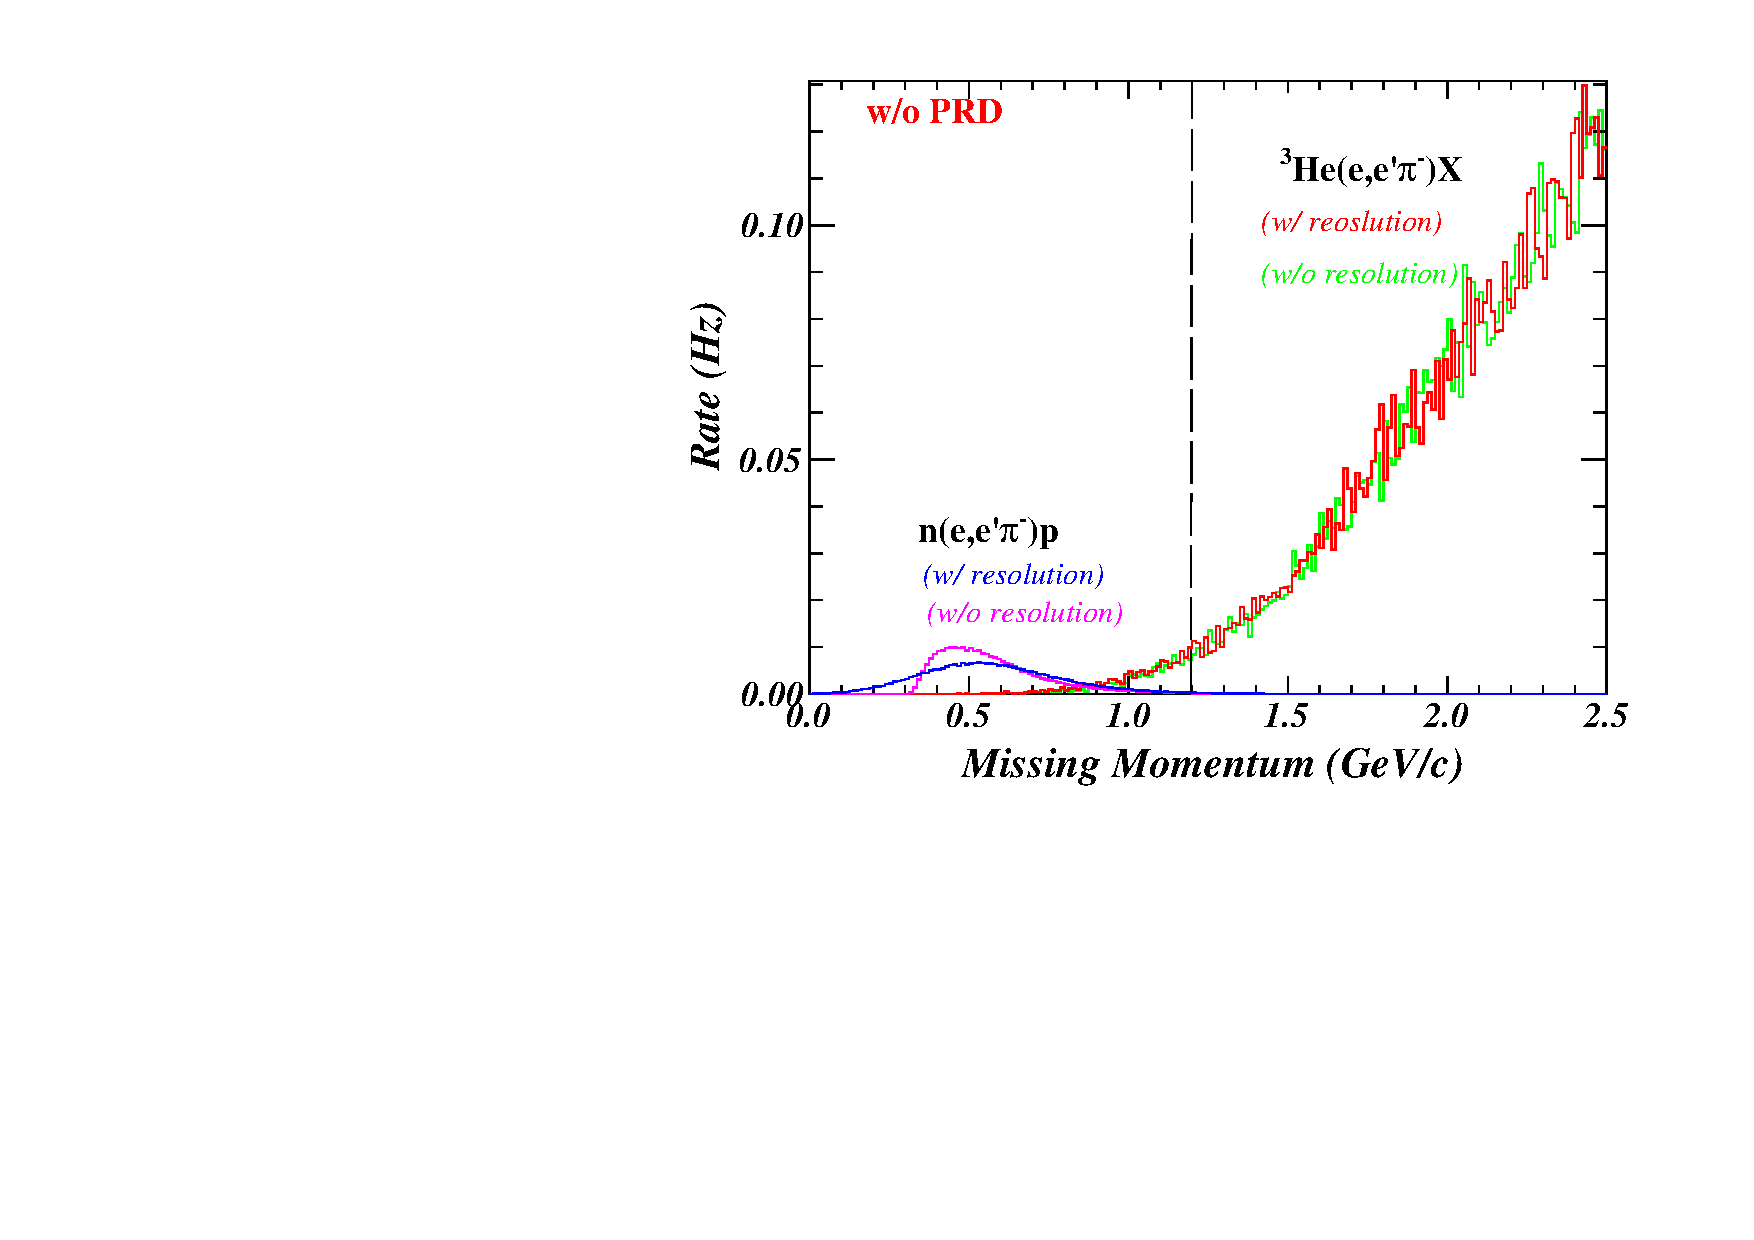
\includegraphics[type=pdf,ext=.pdf,read=.pdf,width=0.5\textwidth]{./figures/Missing_P} }
    \subfloat[w/ PRD]{
      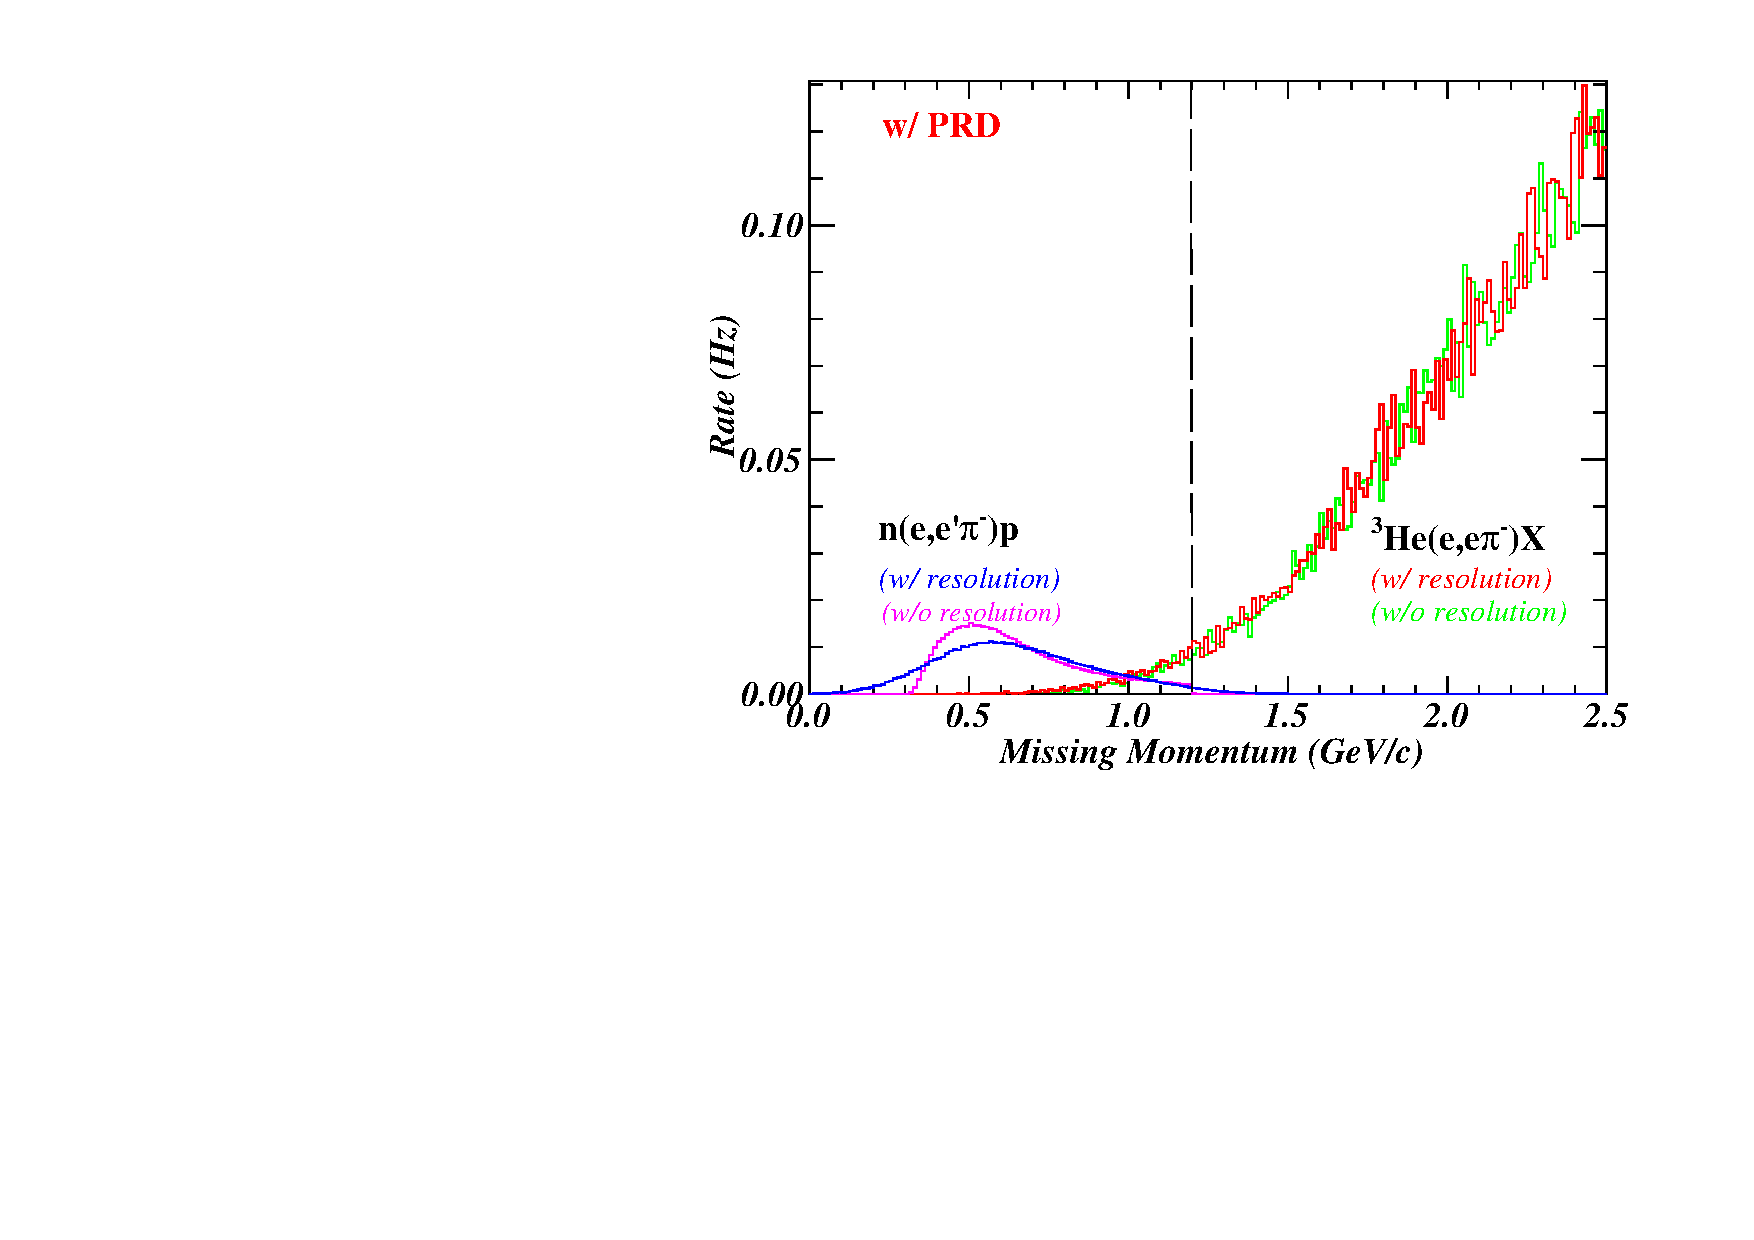
\includegraphics[type=pdf,ext=.pdf,read=.pdf,width=0.5\textwidth]{./figures/Missing_P_prd} } 
   \caption[Missing Momentum]{\footnotesize{Missing momentum spectra of DEMP and SIDIS events. The missing momentum distributes are well separated between two processes and one can apply a cut at $P_{miss}<1.2~GeV/c$ (indicated by the black dash line) to remove most of SIDIS events.}}
  \label{missing_mom}
  \end{center}
\end{figure}
Shown in Fig.~\ref{missing_mom}, we reconstruct the missing momenta of both processes. One immediately sees that the missing momentum distributions of two processes are well separated. The SIDIS background can be largely rejected when we apply a cut, $P_{miss}<1.2~GeV/c$. 

\begin{figure}[!ht]
 \begin{center}
       \subfloat[w/o PRD]{
      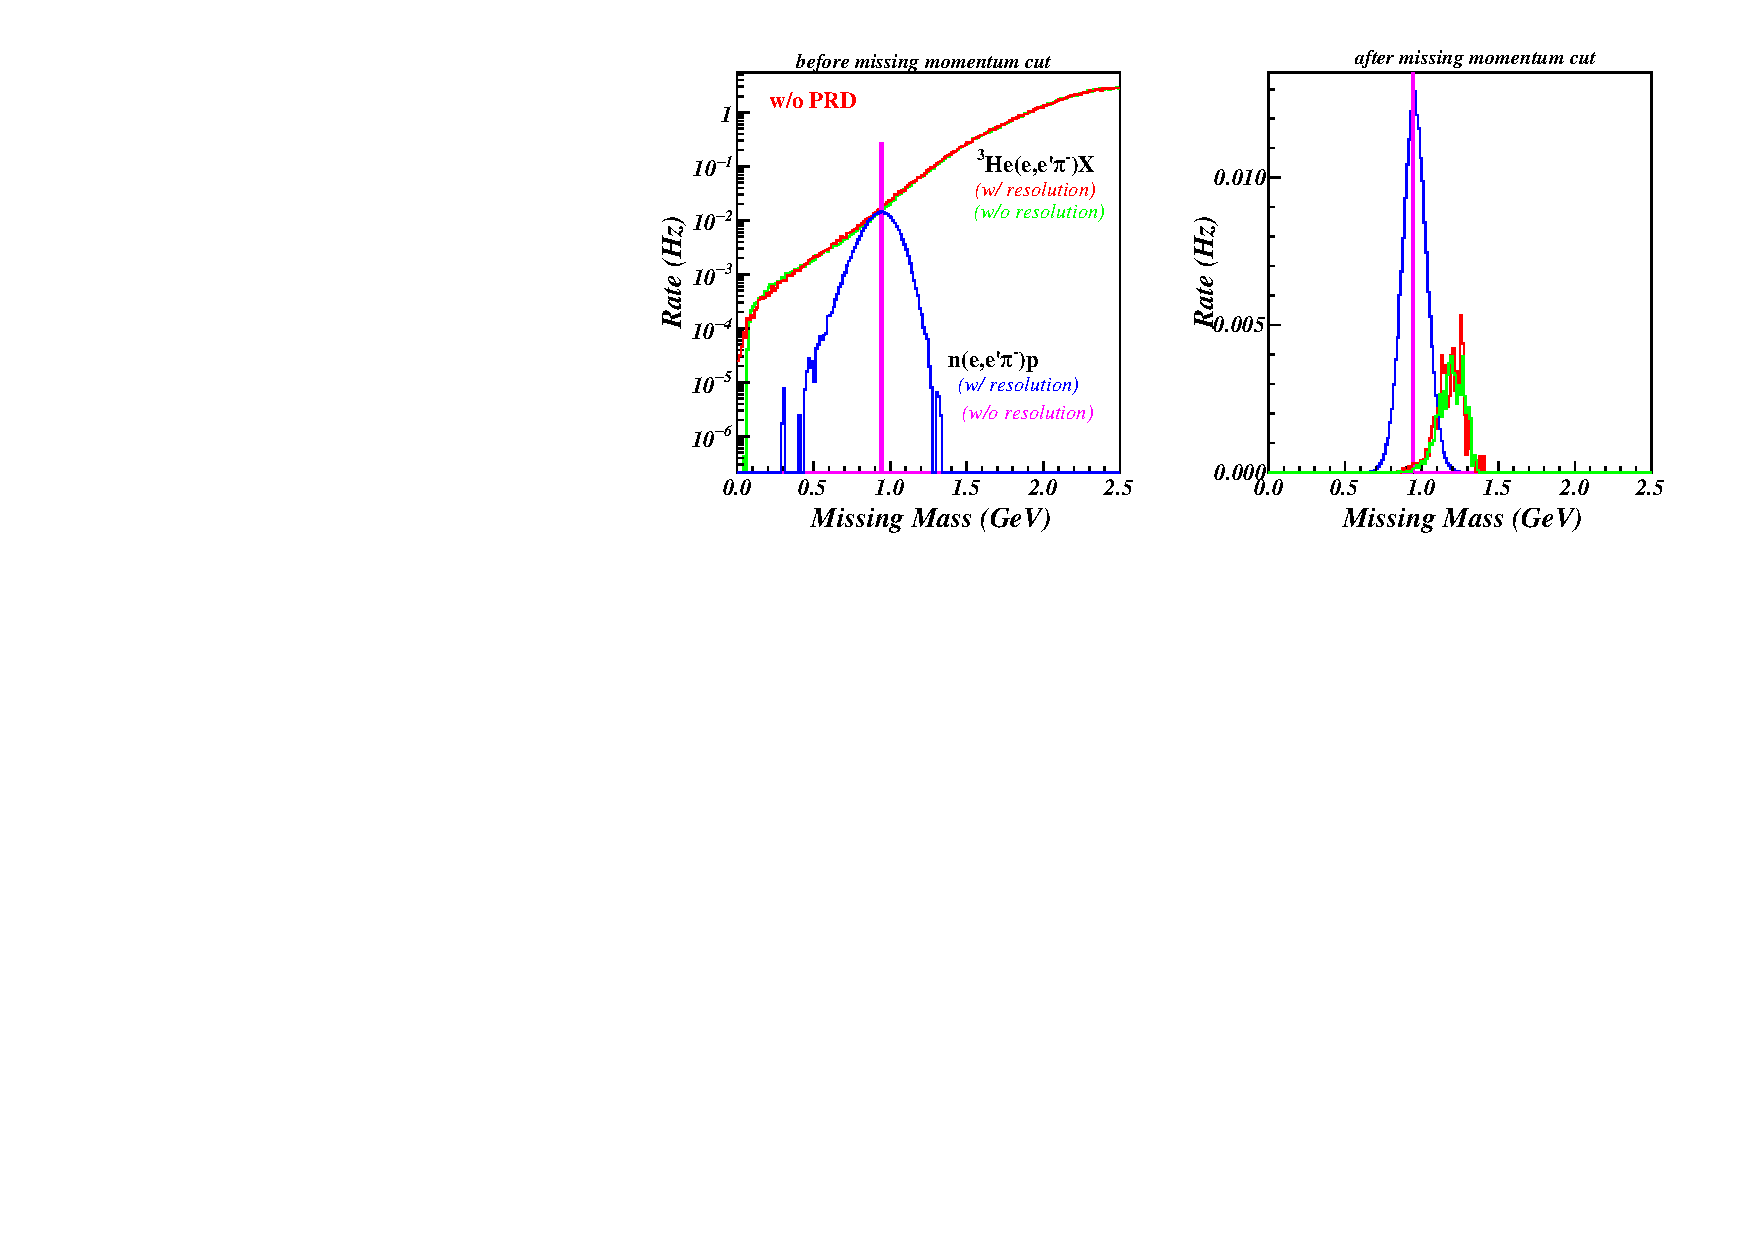
\includegraphics[type=pdf,
        ext=.pdf,read=.pdf,width=0.85\textwidth]{./figures/Missing_Mass} }\\
          \subfloat[w/ PRD]{
      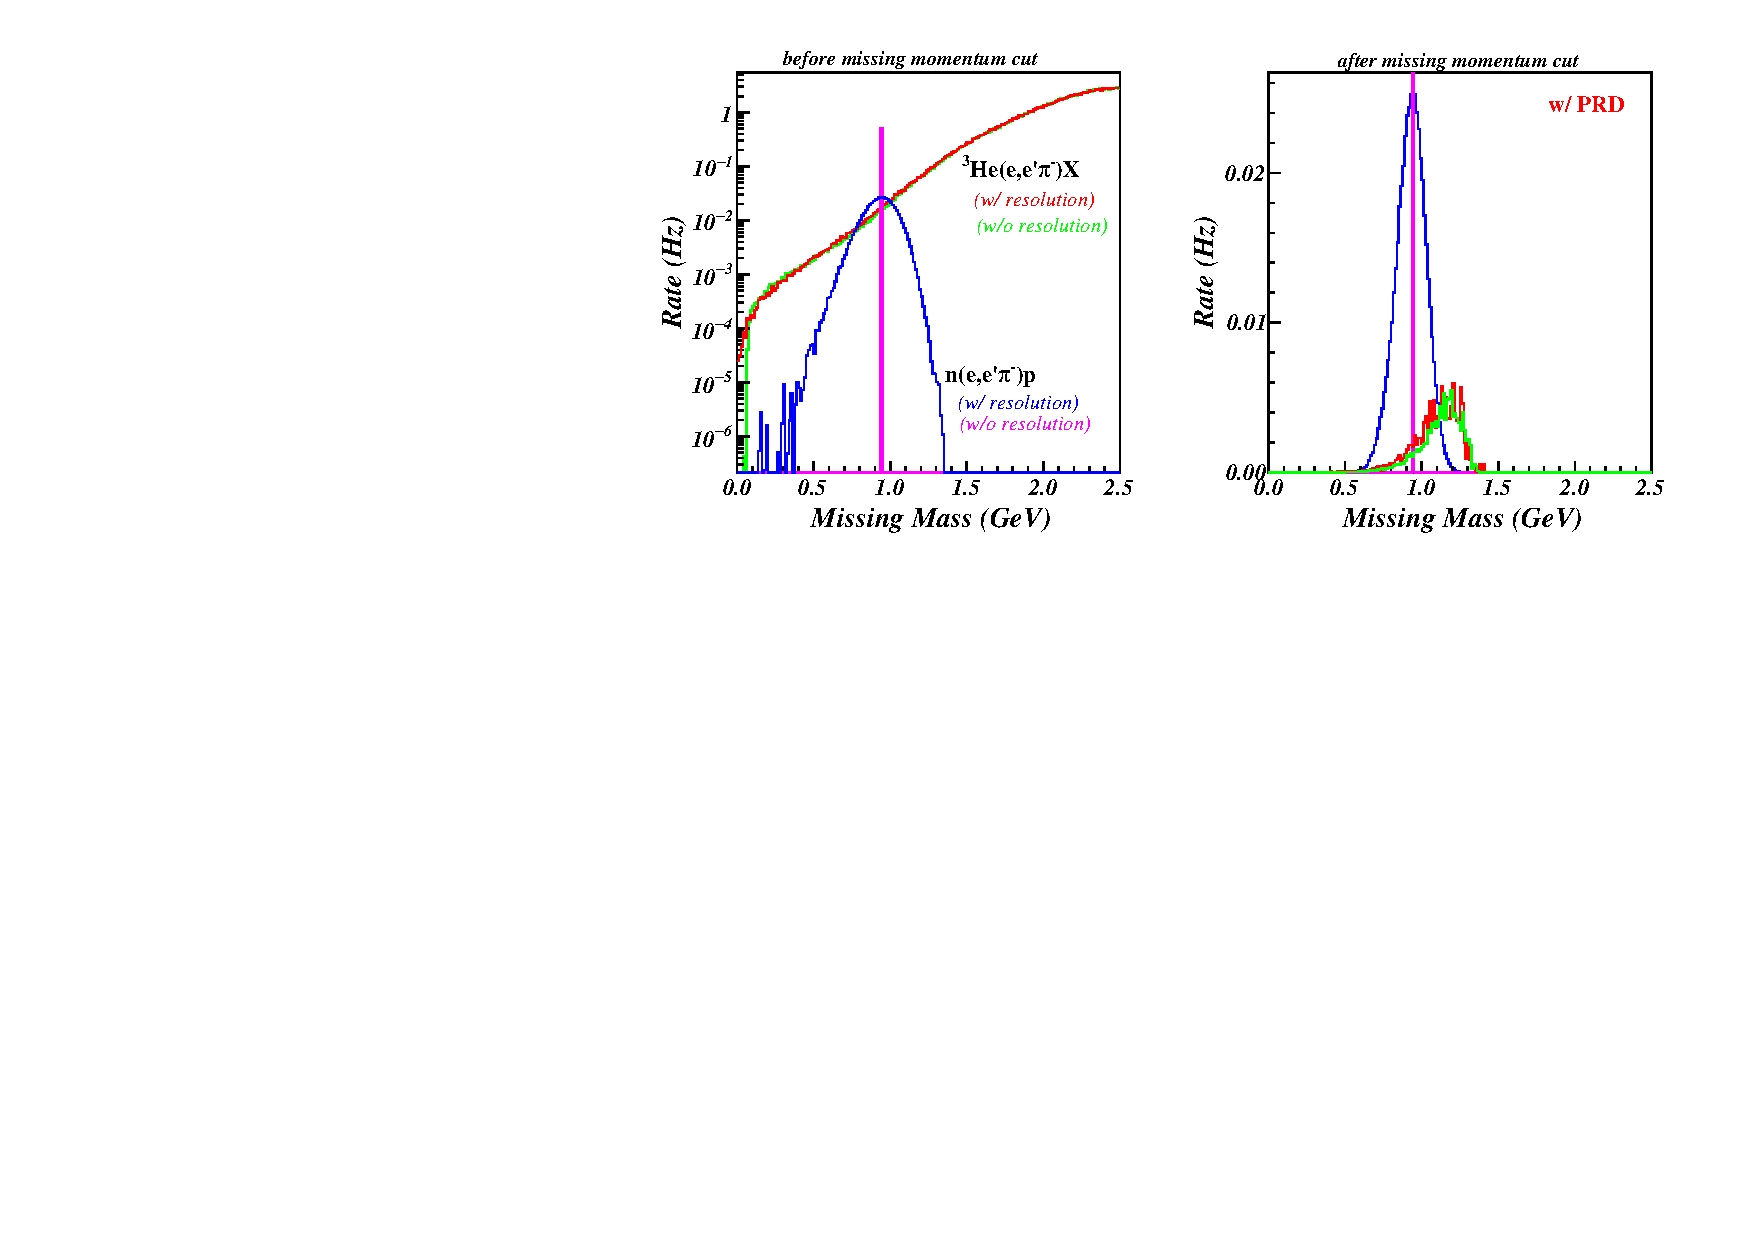
\includegraphics[type=pdf,
        ext=.pdf,read=.pdf,width=0.85\textwidth]{./figures/Missing_Mass_prd} } 
   \caption[Missing Mass]{\footnotesize{Missing mass spectra of DEMP and SIDIS events. Top (bottom) panel shows the missing mass distribution of DEMP events w/o (w/) proton detection by a new PRD. The left (right) plot of each panel shows the background contamination from SIDIS events before (after) the missing momentum cut shown in Fig.~\ref{missing_mom}. The SIDIS background is already small compared with DEMP events. The actual SIDIS background should be much smaller, since we overestimated the SIDIS rate by assuming all target fragments ("X") in the SIDIS process contain protons.}}
  \label{missing_mass}
  \end{center}
\end{figure}

We then reconstructed the missing mass spectra of the DEMP and SIDIS events w/
and w/o the missing momentum cuts, as shown in Fig.~\ref{missing_mass}. Before
applying the missing momentum cut, the SIDIS background overwhelms the DEMP
peak (note that the SIDIS rate is likely overestimated). After applying the
cut, the DEMP peak dominates and the SIDIS background is largely suppressed. If
we consider the fact that not every $``X''$ in SIDIS contains a proton, the
remaining background should be negligible.

Other random coincident background events will show up in the missing mass spectrum with more uniform distributions. We should be able to suppress most of them with tight missing momentum and missing mass cuts, and for these residuals that contaminate the real events, we are able to evaluate their asymmetries if nonzero, and apply corrections on the real asymmetry values. In general, we expect to have a clean measurement of the DEMP process because of all final particles being detected.

\newpage
\section{Summary}

The transverse single-spin asymmetry in the exclusive $\vec{n}(e,e'\pi^-)p$
reaction has been noted as being
especially sensitive to the spin-flip generalized parton distribution (GPD)
$\tilde{E}$.  Factorization studies have indicated that precocious scaling
is likely to set in at moderate $Q^2\sim 2-4$ GeV$^2$, as opposed to the
absolute cross section, where scaling is not expected until $Q^2>10$ GeV$^2$.
Furthermore, this observable has been noted as being important for the reliable
extraction of the charged pion form factor from pion electroproduction.

This measurement is complementary to a proposal 
to measure the longitudinal photon, transverse nucleon, single-spin
asymmetry $A_L^{\perp}$ with the SHMS+HMS in Hall C \cite{atpi39}.  
The good resolution and reproducible systematic uncertainties of the
SHMS+HMS setup allow the L--T separation needed to reliably measure this
quantity.
However, a wide $-t$ coverage is needed to obtain a good understanding of the
asymmetry, and it always been intended to complement the SHMS+HMS $A_L^{\perp}$
measurement with an unseparated $A_{UT}^{sin(\phi-\phi_s)}$ measurement using
a large solid angle detector.  The high luminosity capabilities of SoLID make
it well-suited for this measurement.  Since an L--T separation is not possible
with SoLID, the observed asymmetry is expected to be diluted by the ratio of
the longitudinal cross section to the unseparated cross section.  This was also
true for the pioneering HERMES measurements, which provided a valuable
constraint to models for the $\tilde{E}$ GPD.
Our measurement will also help to constrain longitudinal backgrounds
possibly complicating the extraction of the pion form factor from
electroproduction experiment data, with the aim of eventually extending the
kinematic range over which reliable $F_{\pi}$ values can be acquired from
electroproduction data.


\newpage
\appendix
\section{Monte Carlo model of Deep Exclusive $\pi^{-}$ Production from the
  Neutron in $^{3}$He }

The Monte Carlo studies needed for this proposal require a reaction
model for an experimentally unexplored region of kinematics, at higher
values of $Q^2$, $-t$ and $W$ than covered by existing data.  This appendix
describes the model and the constraints used.

\subsection{Definition of the Cross Section and Single-Spin Asymmetries}

The differential cross section for exclusive $\pi$ production from the nucleon
can be written as
\begin{equation}
  \frac{d^{5} \sigma}{dE' d\Omega_{e'} d\Omega_{\pi}} = \Gamma_{V} \frac{d{^2}
  \sigma}{d\Omega_{\pi}}.
\end{equation}
The virtual photon flux factor $\Gamma_{V}$ is defined as
\begin{equation}
  \Gamma_v=\frac{\alpha}{2\pi^2} \frac{E'}{E} \frac{K}{Q^2}\frac{1}{1-\epsilon},
\end{equation}
where $\alpha$ is the fine structure constant, $K$ is the energy of real photon
equal to the photon energy required to create a system with invariant mass
equal to $W$ and $\epsilon$ is the polarization of the virtual photon.
\begin{equation}
  K=(W^2-M_p^2)/(2 M_p)
\end{equation}
\begin{equation}
  \epsilon=\left(1+\frac{2 |\mathbf{q}|^2}{Q^2} \tan^2\frac{\theta_{e}}{2}
  \right)^{-1},
\end{equation}
where $\theta_{e}$ is the scattering angle of scattered electron.

The two-fold differential cross section $\frac{d{^2} \sigma}{d\Omega_{\pi}}$ in
the lab frame can be expressed in terms of the invariant cross section in
centre of mass frame of the photon and nucleon,
\begin{equation}
  \frac{d^2 \sigma}{d\Omega_\pi}= J \frac{d^2 \sigma}{dt d\phi},
\end{equation}
where $J$ is the Jacobian of transformation of coordinates from lab
$\Omega_{\pi}$ to $t$ and $\phi$ (CM). 

Following Ref.~\cite{hermes-thesis}, we consider separately the unpolarized and
polarized target contributions to the invariant photon nucleon cross section,
\begin{equation}
  d\sigma = d\sigma_{UU} + d\sigma_{UT}.
  \label{eqn:cross-1}
\end{equation}

In the one-photon exchange approximation, the unpolarized nucleon 
cross section for $n(e,e^{\prime}\pi^{-})p$
can be expressed in four terms. Two terms correspond
to the polarization states of the virtual photon (L and T) and two states
correspond to the interference of polarization states (LT and TT),
\begin{equation}
  d\sigma_{UU} =  \epsilon  \frac{d\sigma_{\mathrm{L}}}{dt}
  + \frac{d\sigma_{\mathrm{T}}}{dt} + 
  \sqrt{2\epsilon (\epsilon +1)} \frac{d\sigma_{\mathrm{LT}}}{dt} \cos{\phi}
  + \epsilon  \frac{d\sigma_{\mathrm{TT}}}{dt} \cos{2 \phi},
  \label{eqn:cross-2}
\end{equation}
where $\phi$ is the angle between lepton plane and hadron plane
(Fig.~\ref{fig:planes}). 
The first two terms of Eqn.~\ref{eqn:cross-2} correspond to the
polarization states of the virtual photon (L and T) and last two terms
correspond to the interference of polarization states (LT and TT).  $\epsilon$
is the ratio of longitudinal to transverse virtual-photon fluxes
\begin{equation}
  \epsilon=\left(1+\frac{2
  |\mathbf{q}|^2}{Q^2} \tan^2\frac{\theta_{e}}{2} \right)^{-1}.
\end{equation}
The constraints used to parameterize $d\sigma_{UU}$ are described in
Sec.~\ref{sec:model}.

The additional contribution when the target nucleon is transversely polarized
can be parameterized \cite{Di05,hermes-thesis} as
\begin{equation}
  d\sigma_{UT} = -\frac{P_{T}}{\sqrt{1 - \sin^{2}{\theta} \sin^{2}{\phi_{S}} }
  } \sum_{k=1}^{6} \sin{ (\mu\phi + \lambda\phi_{S})
  } \Sigma_{k},
\label{eqn:cross-3}
\end{equation}
where $\phi_{S}$ is angle between the target polarization and lepton planes
(Fig.~\ref{fig:planes}), the $\Sigma_{k}$ are given by
\begin{equation}
  \Sigma_{k} = A_{UT}^{\sin{( \mu\phi+\lambda\phi_{S})_{k}}} \times
  d\sigma_{UU}(\phi),
  \label{eqn:sigmas}
\end{equation}
and the $\sin (\mu\phi + \lambda\phi_{S})$ are the different azimuthal
modulations.  The calculation of $d\sigma_{UT}$ in the event generator is
described in Sec.~\ref{sec:asymparametrizations}.

\subsection{Cross Section Model for Higher $Q^2$ Kinematics
\label{sec:model}}

\subsubsection{Constraints}

All of the following data were used as constraints on the parameterizations
used in this model.
\begin{itemize}
\item
From Hall C, precise $L/T$ separated experimental data of exclusive
electroproduction of $\pi^{-}$ on $^2$H are available up to $Q^2=2.57$ GeV$^2$,
$-t=0.350$ GeV$^2$ and $W=2.168$ GeV \cite{gmhuber-2}.
\item
Also from Hall C, precise $L/T$ separated experimental data of exclusive
electroproduction of $\pi^{+}$ on $^1$H are available up to $Q^2=2.703$
GeV$^2$, $-t=0.365$ GeV$^2$ and $W=2.127$ GeV \cite{Fpi2}, and separated
$\sigma_{L}$ and $\sigma_{T}$ are measured up to $Q^2=4.703$ GeV$^2$ and
$W=2.2$ GeV \cite{hallc-1} and \cite{hallc-2}.
\item
CLAS experiment E99-105 measured the unseparated exclusive $\pi^+$ cross
section from $^1$H at $Q^2$ up to $4.35$ GeV$^2$ and $-t$ up to $4.5$ GeV$^2$
\cite{park}.
\item
The HERMES collaboration measured the unseparated cross section for $Q^2$=3.44
GeV$^2$ and 5.4 GeV$^2$ \cite{hermes} at $W$=4 GeV.
\end{itemize}

An additional constraint in our parameterization comes from the
Vrancx-Ryckebusch (VR) model \cite{vr}.  This is a Regge model with a
parametrization of the deep inelastic scattering amplitude added to improve the
description of $\sigma_{T}$.  The description of $\sigma_{L}$ in the model is
constrained by a fit to the Hall C $p(e,e'\pi^+)n$ data from
Ref.~\cite{gmhuber}.  The model provides a good description of exclusive
charged pion electroproduction above the resonance region.  It has been checked
for reliability against the Hall B and C data listed above, for $W>2$ GeV,
$Q^2$ from 0.35 to 4.98 GeV$^2$.  The model is believed to be reliable for
$-t\leq$0.5 GeV$^2$, but it overshoots the data for $-t>$0.5 GeV$^2$.

\begin{figure}[!hbt]
    \centering
    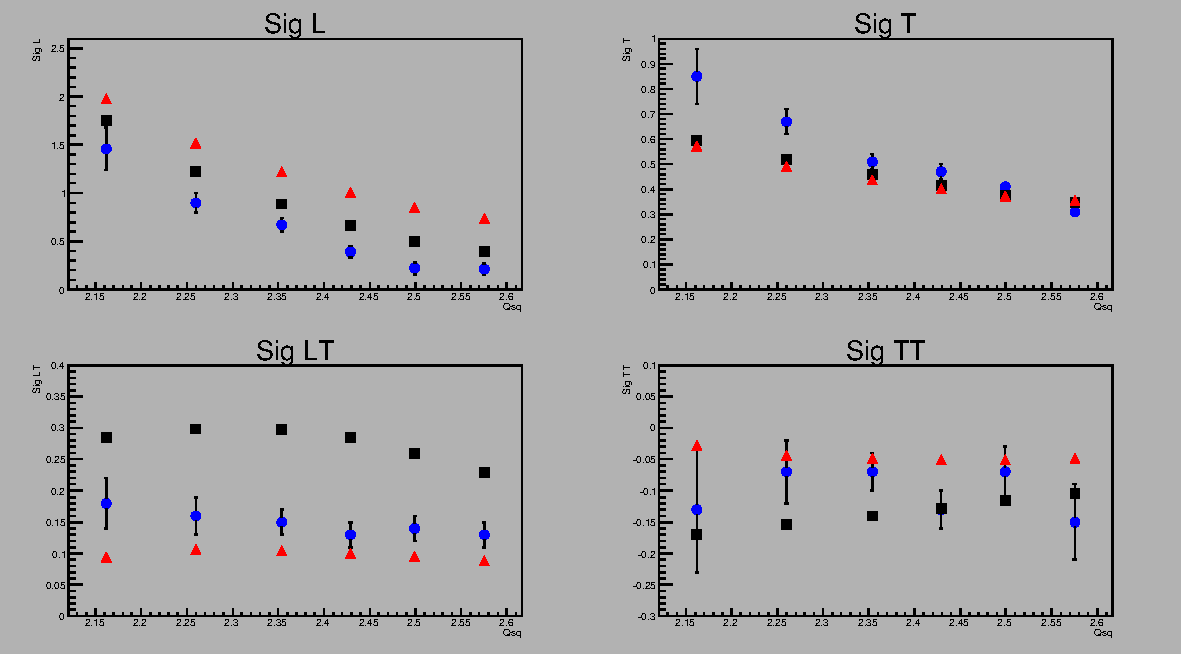
\includegraphics[width=6.0in,height=2.4in]{./figures/pimsigma_qsq.pdf}
%    \includegraphics[width=6.0in,height=3.0in]{./figures/01.eps}
    \caption{ A comparison of last six points of table $v$ of \cite{gmhuber-2},
      the VR model, and our parametrization values vs. $Q^{2}$ for $\pi^{-}$
      electroproduction. Experimental data are shown in blue circles, VR model
      is shown in red triangles, and our parametrization is shown in black
      boxes. In each graph, the value of $-t$ is decreasing left to right from
      a maximum value 0.35 GeV$^2$ to 0.15 GeV$^2$. Value of $W$ also decreases
      left to Right from 2.2978 GeV to 2.1688 GeV.}
    \label{fig:expvrfit}
\end{figure}

\begin{figure}[!hbt]
    \centering
\    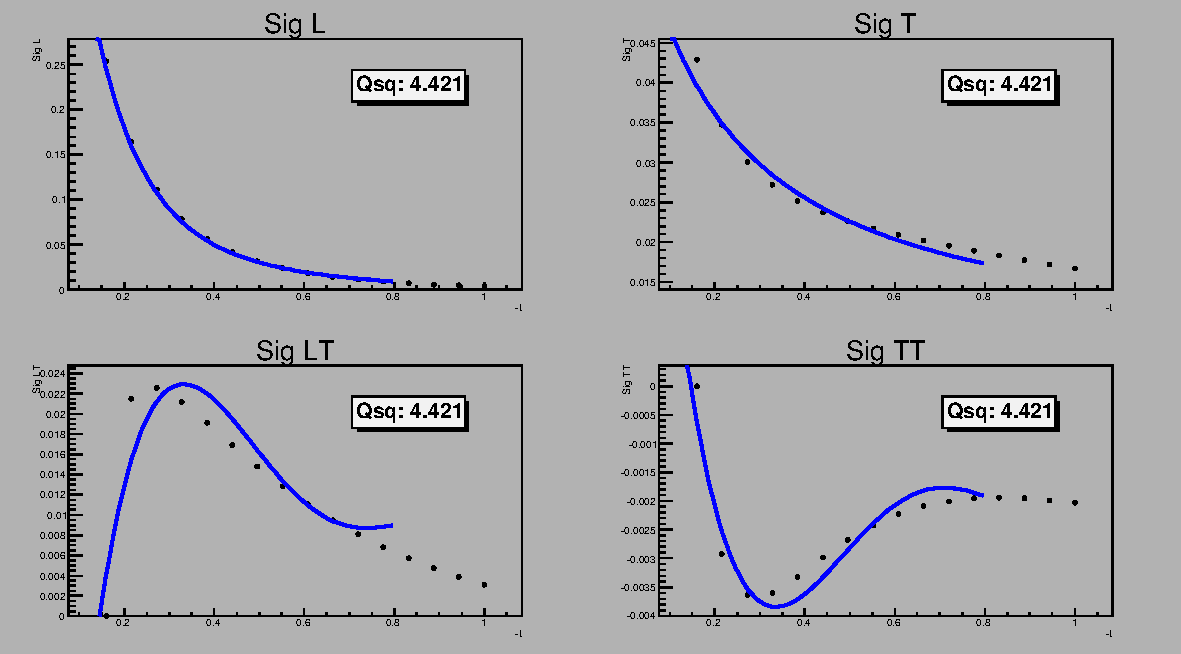
\includegraphics[width=6.0in,height=2.4in]{./figures/pimFit.pdf}
%    \includegraphics[width=5.0in,height=2.4in]{./figures/02.eps}
    \caption{ A comparison of parametrized $\sigma_{L,T,LT,TT}$ and VR model
    values at $Q^2$ = 4.421 GeV$^2$ and $W = 3.0$ GeV.  Black points are VR
    model values and blue line is parametrized $\sigma_{L,T,LT,TT}$ given by
    equations $\ref{equation:l-fit}$ to $\ref{equation:tt-fit}$. }
    \label{fig:sigall}
\end{figure}

\subsubsection{Parametrization of $\sigma_{L}$, $\sigma_{T}$, $\sigma_{LT}$, 
$\&$ $\sigma_{TT}$
\label{sec:parametrization}}

For exclusive DEMP in SoLID, the kinematic region of interest for
parametrization of $\sigma_{L,T,LT,TT}$ is $Q^2$ from 4.0 GeV to 7.5 GeV$^2$,
$-t$ from 0 GeV$^2$ to 1.0 GeV$^2$, and we set $W=3.0$ GeV. After the
parametrization of $\sigma_{L,T,LT,TT}$ for $-t$ and $Q^2$, we used the same
$W$ dependence given by \cite{gmhuber}, which is $(W^2-M^2)^{-2}$ where $M$ is
the proton mass.  Our parametrization of all four cross sections is given in
equations $\ref{equation:l-fit}$ to $\ref{equation:tt-fit}$.

\begin{equation}
        \sigma_{L} = \exp{(P_1(Q^2) + |t| * P^{\prime}_1(Q^2))}
        + \exp{(P_2(Q^2) + |t| * P^{\prime}_2(Q^2))}
     \label{equation:l-fit}
\end{equation}

\begin{equation}
        \sigma_{T} = \frac{\exp{(P_1(Q^2) + |t| *
        P^{\prime}_1(Q^2))}}{P_{1}(|t|)}
     \label{equation:t-fit}
\end{equation}

\begin{equation}
        \sigma_{LT} = P_{5}(t(Q^2))
     \label{equation:lt-fit}
\end{equation}

\begin{equation}
        \sigma_{TT} = P_{5}(t(Q^2))       
     \label{equation:tt-fit}
\end{equation}

Here, the parameters $P_{i}$ are polynomial functions of $i^{th}$ order. Each
coefficient ($P_{i}$) of the fifth order equations $\ref{equation:lt-fit}$ and
$\ref{equation:tt-fit}$ is a further second order polynomial of $Q^2$. Deep
exclusive $\pi^{-}$ events are generated using a C++ code. The quality of
parametrization is checked by plotting the parametrization functions of
$\sigma_{L,T,LT,TT}$ versus the existing data and the VR model are shown in 
Figs. \ref{fig:expvrfit}, \ref{fig:sigall}.

{\bf There is no statement made that the cross section is calculated in the
  neutron rest frame from the `vertex' kinematic quantities, and then
  transformed to the lab frame.}

\subsection{Parametrization of six Single-Spin Asymmetries
\label{sec:asymparametrizations}}

\begin{figure}[!hbt]
    \centering
    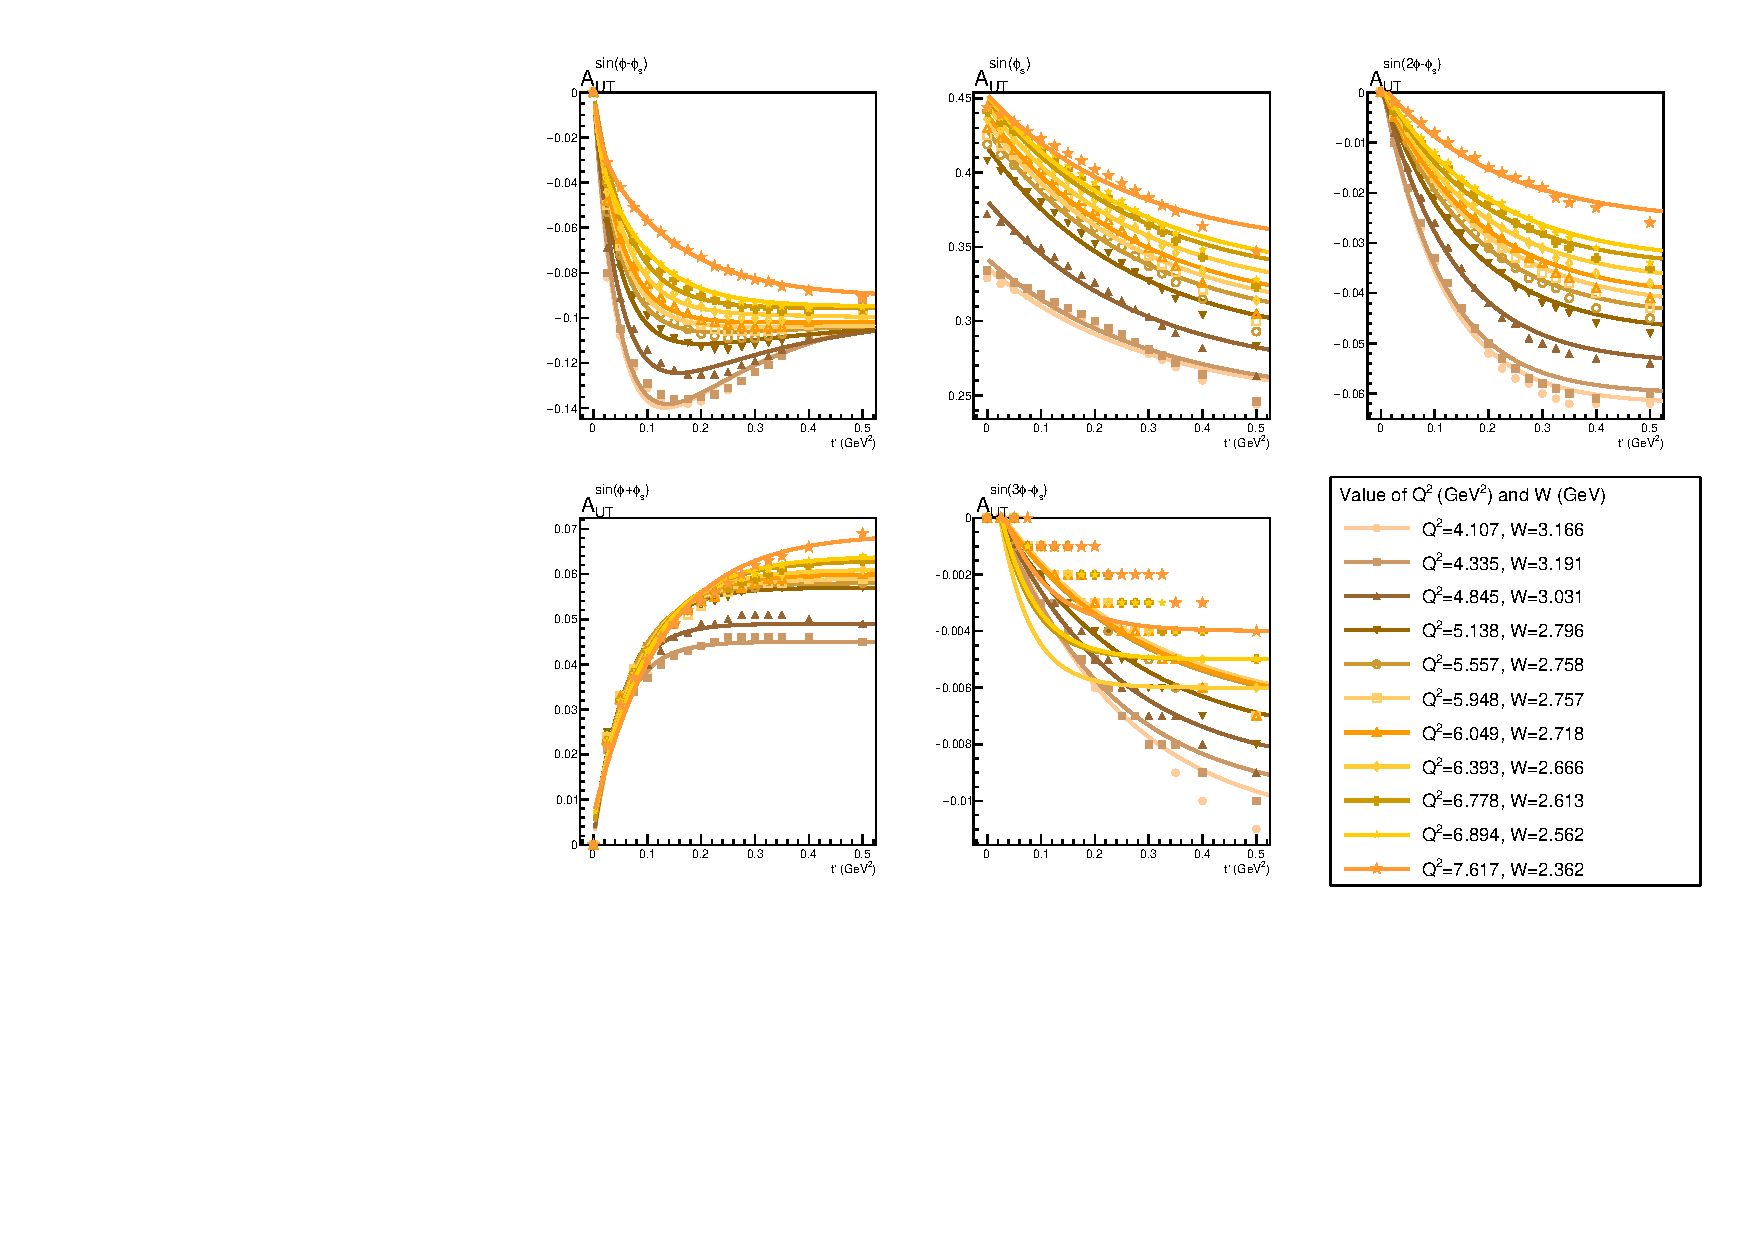
\includegraphics[width=6.0in]{./figures/AsymPlots.pdf}
    \caption{Parametrization of the five single spin asymmetries
      $A_{UT}^{\sin(\mu\phi+\lambda\phi_s)_k}$ vs. $t'$ used in the event
      generator for this proposal.  The points are the calculations by
      Goloskokov and Kroll \cite{GoPC} and the curves are our fit.}
    \label{fig:asym-1}
\end{figure}

The single-spin asymmetries calculated for us by S.V Goloskokov and P. Kroll
\cite{GoPC} have been used to approximate $d\sigma_{UT}$ in the
DEMP event generator.  Their $A_{UT}^{\sin(\mu\phi+\lambda\phi_s)_k}$ values are
at discrete values of $Q^2$ from 4.107 to 7.167~GeV$^2$, $W$ from 2.362 to
3.191~GeV, and $t'$ from 0~GeV$^2$ to 0.5~GeV$^2$.  There are six different 
azimuthal modulations defined as follows:
\begin{center}
\begin{tabular}{ l|l }
  $k$ & $\sin(\mu\phi+\lambda\phi_s)$ \\
  \hline
  $1$ & $\sin(\phi-\phi_s)$ \\
  $2$ & $\sin(\phi+\phi_s)$ \\
  $3$ & $\sin(\phi_s)$ \\
  $4$ & $\sin(2\phi-\phi_s)$ \\
  $5$ & $\sin(3\phi-\phi_s)$ \\
  $6$ & $\sin(2\phi+\phi_s)$
\end{tabular}
\end{center}

These asymmetries are used to give
\begin{align}
  \Sigma_k &= d\sigma_{UU}(\phi)A_{UT}^{\sin(\mu\phi+\lambda\phi_s)_k} \\
  d\sigma_{UT}&=-\frac{P_T}{\sqrt{1-\sin^2\theta
      \sin^2\phi_s}}\sum_{k=1}^{6}\sin(\mu\phi+\lambda\phi_s)_k\Sigma_k
\end{align}

The $k=6$ asymmetry ($(\mu,\lambda)=(2,1)$) is not included in their
calculation, and is taken to be zero, in accordance with the HERMES data
\cite{hermes-thesis}. The other five are calculated based on fits to their
values.  The following fits were used:
\begin{align}
  A_{UT}^{\sin(\mu\phi+\lambda\phi_s)_k} =
  \begin{cases}
    ae^{bx}-(a+c)e^{dx}+c, &\quad k=1 \\
    ae^{bx}+c, &\quad k=2,3,4,5
  \end{cases}
\end{align}
where $a$, $b$, $c$, and $d$ are fit parameters. The forms of these functions
were chosen only to closely match the shape of the simulated data and are not
based on any physical principle. These fits are done for each given value of
$Q^2$ independently, as shown in Fig.~\ref{fig:asym-1}.  During event
generation, the asymmetry is calculated from the fit for the two nearest values
of $Q^2$. The asymmetry for the given event is then approximated by linear
interpolation of the nearest values.

\subsection{Target Neutron Fermi Momentum 
\label{sec:fermimotion}}

\begin{figure}[!hbt]
    \centering
    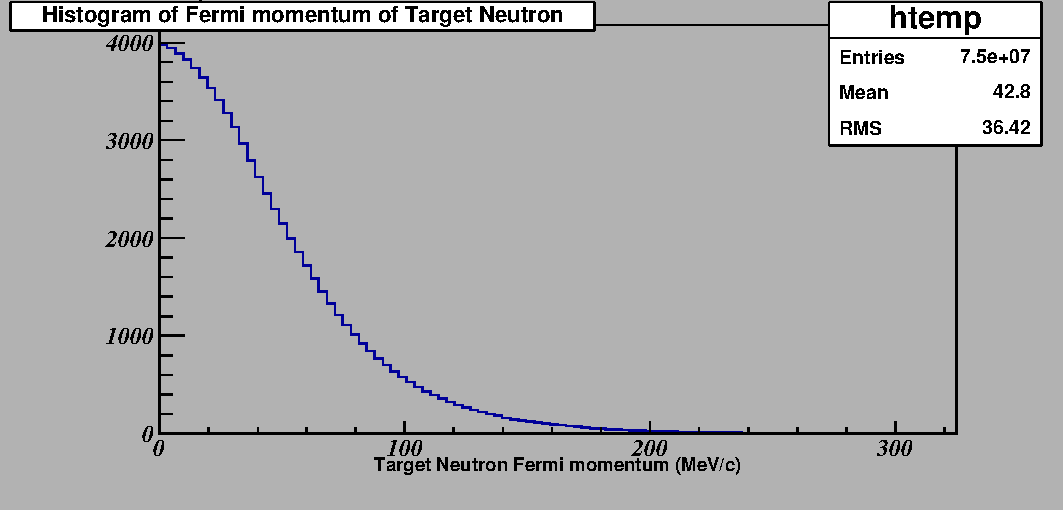
\includegraphics[width=4.0in,height=2.5in]{./figures/Fermi.pdf}
%    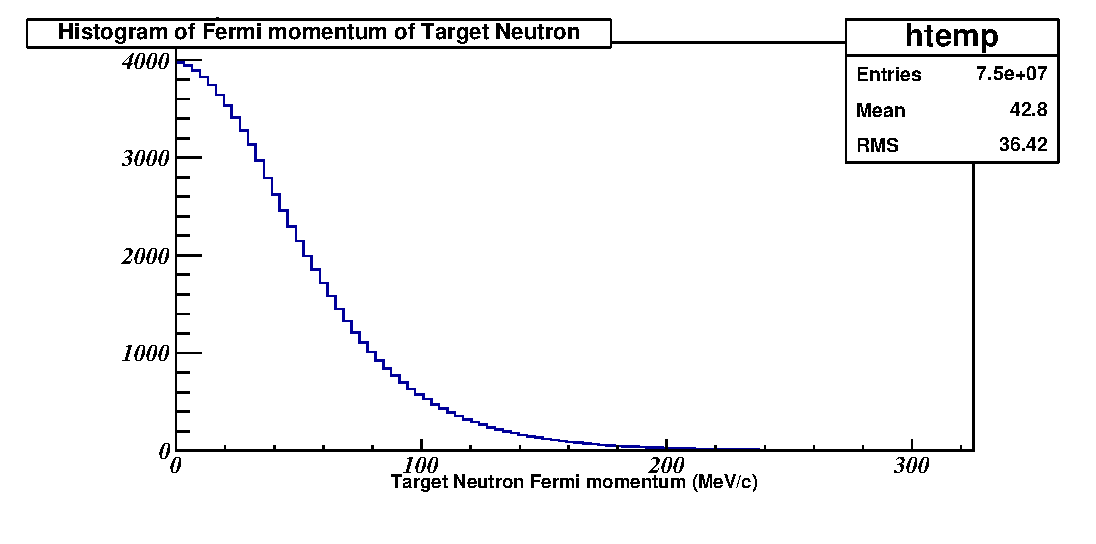
\includegraphics[width=4.0in,height=2.5in]{04.eps}
    \caption{Fermi momentum spectral function of a target nucleon in $^3$He
      generated according to the Argonne potential of Ref \cite{fermipaper}.
      The horizontal axis is nucleon momentum in MeV/c.}
    \label{fig:fermi}
\end{figure}

A histogram of the spectral function of $^3$He is shown in
Fig.~\ref{fig:fermi}, generated according to Ref.~\cite{fermipaper}. Neutron
momenta up to 300 MeV/c are generated according to this distribution, uniformly
distributed in spherical coordinates. The quasi-free collision between the
virtual photon and moving neutron is then transformed to the fixed neutron
frame, after which the parameterizations of Secs.~\ref{sec:parametrization},
\ref{sec:asymparametrizations} are applied. The outgoing particles are then
transformed back to the lab frame for tracking.

\subsection{Energy Loss and Multiple Scattering
\label{sec:energyloss}}

There is energy loss for the incoming electron $e$, and the three outgoing
particles: scattered electron $e^{\prime}$, $\pi^{-}$ and recoil proton $p$ by
bremsstrahlung and ionization.  The same code as given in SAMC (Hall A Single
Arm Monte Carlo) \cite{samc} is used.  This code is based on Sec. 33 (Passage
of articles through matter) of the Review of Particle Physics by the Particle
Data Group \cite{pdg}.

Incoming electron and three out going particles are deflected small angles by
multiple scattering in the target, target window and in the air. This small
deflection in the polar angle theta $\theta$ is calculated according to
Subsection 33.3 (Multiple scattering through small angles) of the Review of Particle
Physics by the Particle Data Group \cite{pdg}.

The incoming electron loses energy by bremsstrahlung and ionization, and
suffers multiple scattering, in the target and in the target window.  Both of
these processes and the choice of neutron Fermi momentum are applied before the
cross section terms $\sigma_{uu}$ and $\sigma_{UT}$ are calculated from the
`vertex' kinematic quantities.

The scattered electron, pion and proton lose energy by bremsstrahlung and
ionization, and suffer multiple scattering, in the target, target window and in
the air.  The energy and momentum of these particles are corrected according to
these processes prior to particle tracking.

\subsection{Final State Interactions
\label{sec:fsi}}

A separate version of the model was made in which the outgoing $\pi^-$ suffers
$\pi N$ final state interactions (FSI) with one of the recoil $p$ in the
residual nucleus.

The scattering of $\pi^-$ by protons involves both the $T=1/2$ and $T=3/2$
isospin states.  We model the $\pi^- p$ scattering via the empirical phase
shift analysis of Rowe, Solomon and Landau \cite{rowe}.  In this case,
the amplitude for the scattering of a spin-zero particle by a particle of
spin-$\frac{1}{2}$ is described for each isospin channel by a set of partial
wave amplitudes $f^{(+)}_{\ell}$, $f^{(-)}_{\ell}$ for the
$j=\ell\pm\frac{1}{2}$ states.  In terms of phase shifts, $f^{(+)}_{\ell}$ is
\begin{equation}
f^{(+)}_{\ell}\equiv\frac{1}{2ik}(e^{2i\delta^+_{\ell}} -1)
\end{equation}
with a similar expression for $f^{(-)}_{\ell}$.  The phase shift
$\delta^+_{\ell}$ will be complex if there is any inelasticity, which will
occur for example for the reactions
\begin{equation}
\begin{split}
\pi^- + p &\rightarrow \pi^+ \pi^- p \\
          &\rightarrow \pi^0 \pi^0 n \\
          &\rightarrow \pi^- \pi^0 p. \\
\end{split}
\end{equation}
The differential cross-section is written in terms of these phase shifts as
\begin{equation}
\frac{d\sigma}{d\Omega}=\biggl[
\biggl| \frac{1}{k}\sum_{\ell}[(\ell +1) 
f^{(+)}_{\ell} +\ell f^{(-)}_{\ell}] P_{\ell}(\cos\theta)\biggr|^2 +
\biggl| \frac{i}{k}\sum_{\ell}[f^{(+)}_{\ell} -f^{(-)}_{\ell}]\sin\theta 
 \frac{d P_{\ell}(\cos\theta)}{d\cos\theta}\biggr|^2
\biggr].
\label{eqn:piN}
\end{equation}

$\pi N$ phase shifts have been determined experimentally from near threshold up
to several GeV.  The dominant phase shifts for the $L_{2T,2J}$ states:
S$_{11}$, S$_{31}$, P$_{11}$, P$_{13}$, P$_{31}$, P$_{33}$ are very accurately
known for centre of mass momenta up to 350 MeV/c.  The phase shift
parameterizations used in our model are dominated by the $\Delta(1232)$ and
$N^*(1440)$ resonances.  For further information, please see
Ref.~\cite{ericson}.

In our implementation of the FSI process, the Fermi momentum of one of the
recoil protons was chosen according to Sec.~\ref{sec:fermimotion} and collided
with the outgoing $\pi^-$ in their mutual centre of mass frame.  Outgoing
$\pi^-$ $N$ were randomly generated, and the events
weighted according to the differential cross setions of Eqn.~\ref{eqn:piN}.
Events were generated for both the FSI and non-FSI versions of the
model and the results compared, as described in the main text.

%\section{Proton Recoil Detector}


\section{Improvment to Projection of new Measurement}
\begin{figure}[!ht]
 \begin{center}
    \subfloat[w/o PRD]{
      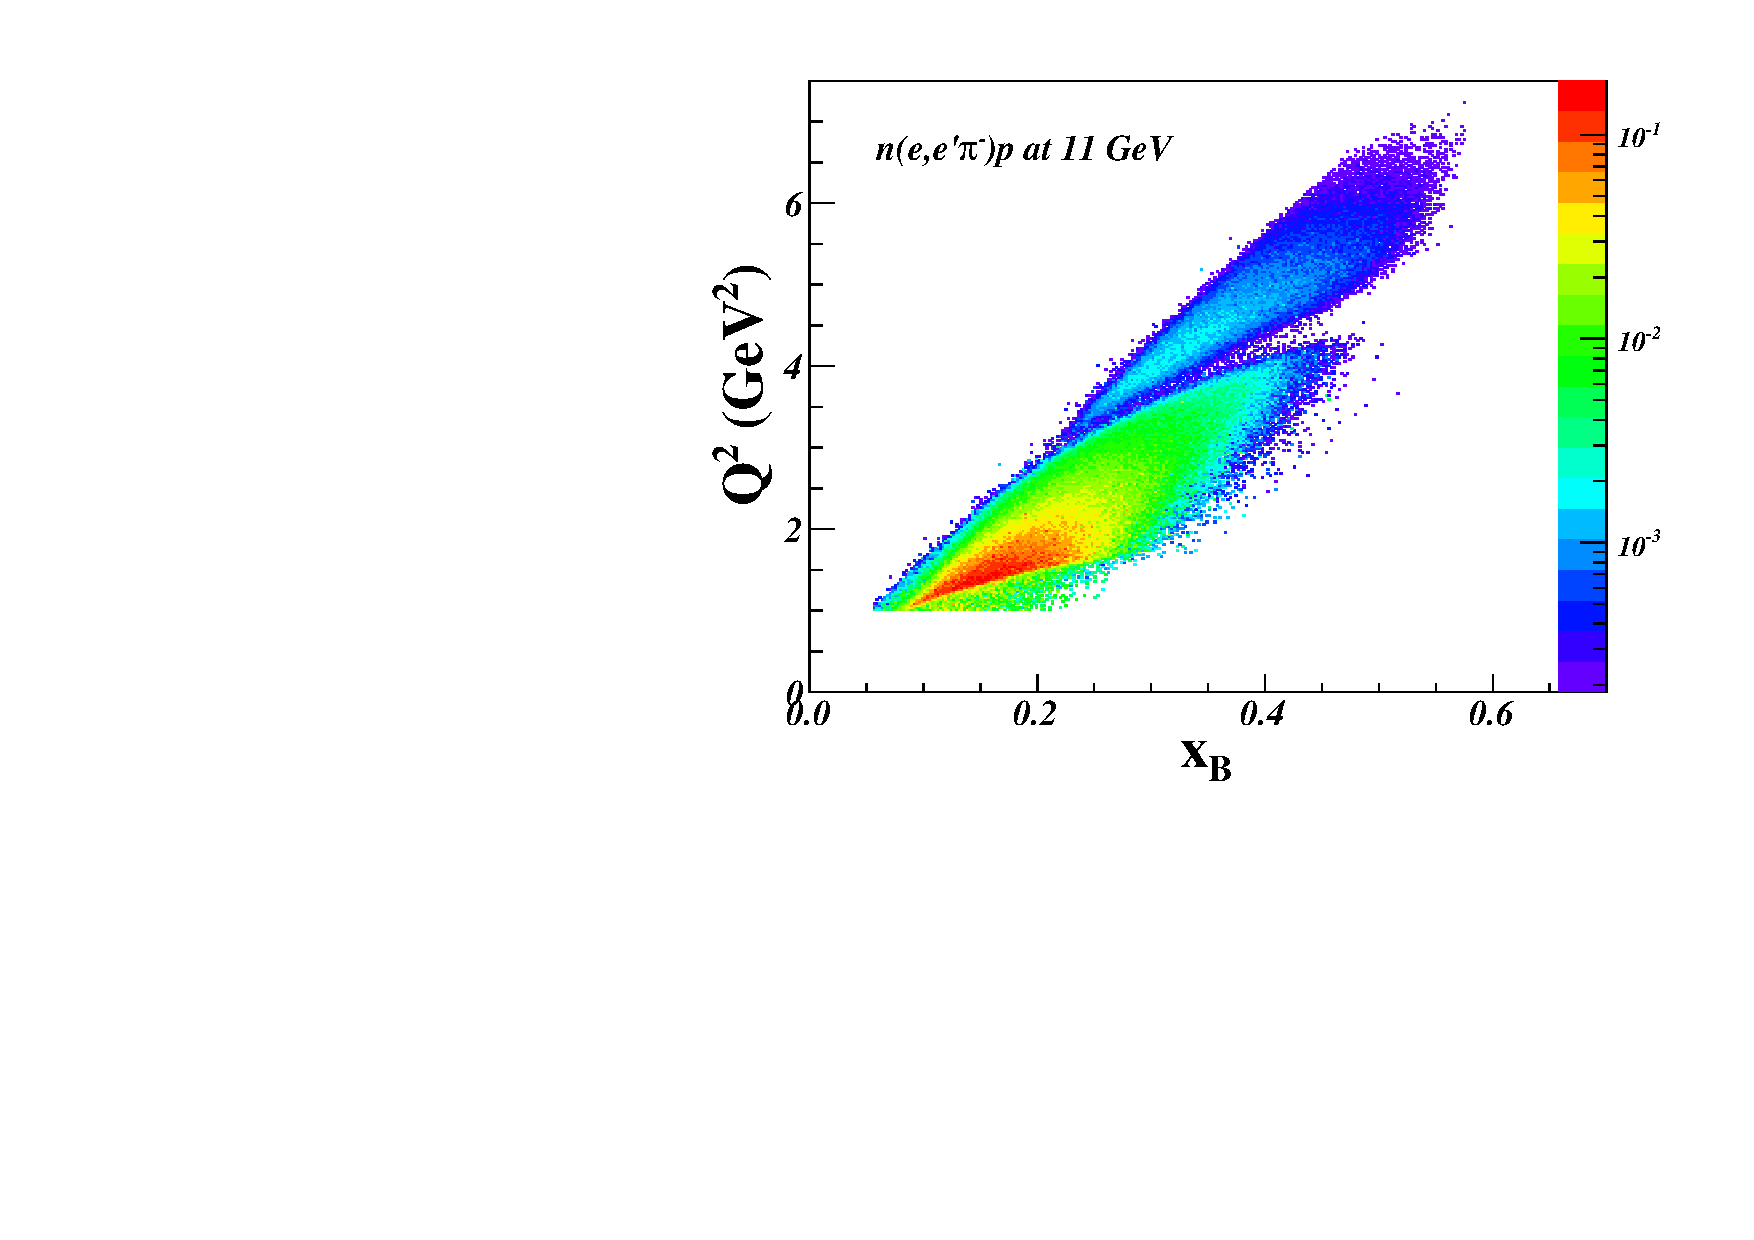
\includegraphics[type=pdf,
        ext=.pdf,read=.pdf,width=0.45\textwidth]{./figures/E11_Q2_x_fermi}
         }
           \subfloat[w/ PRD]{
      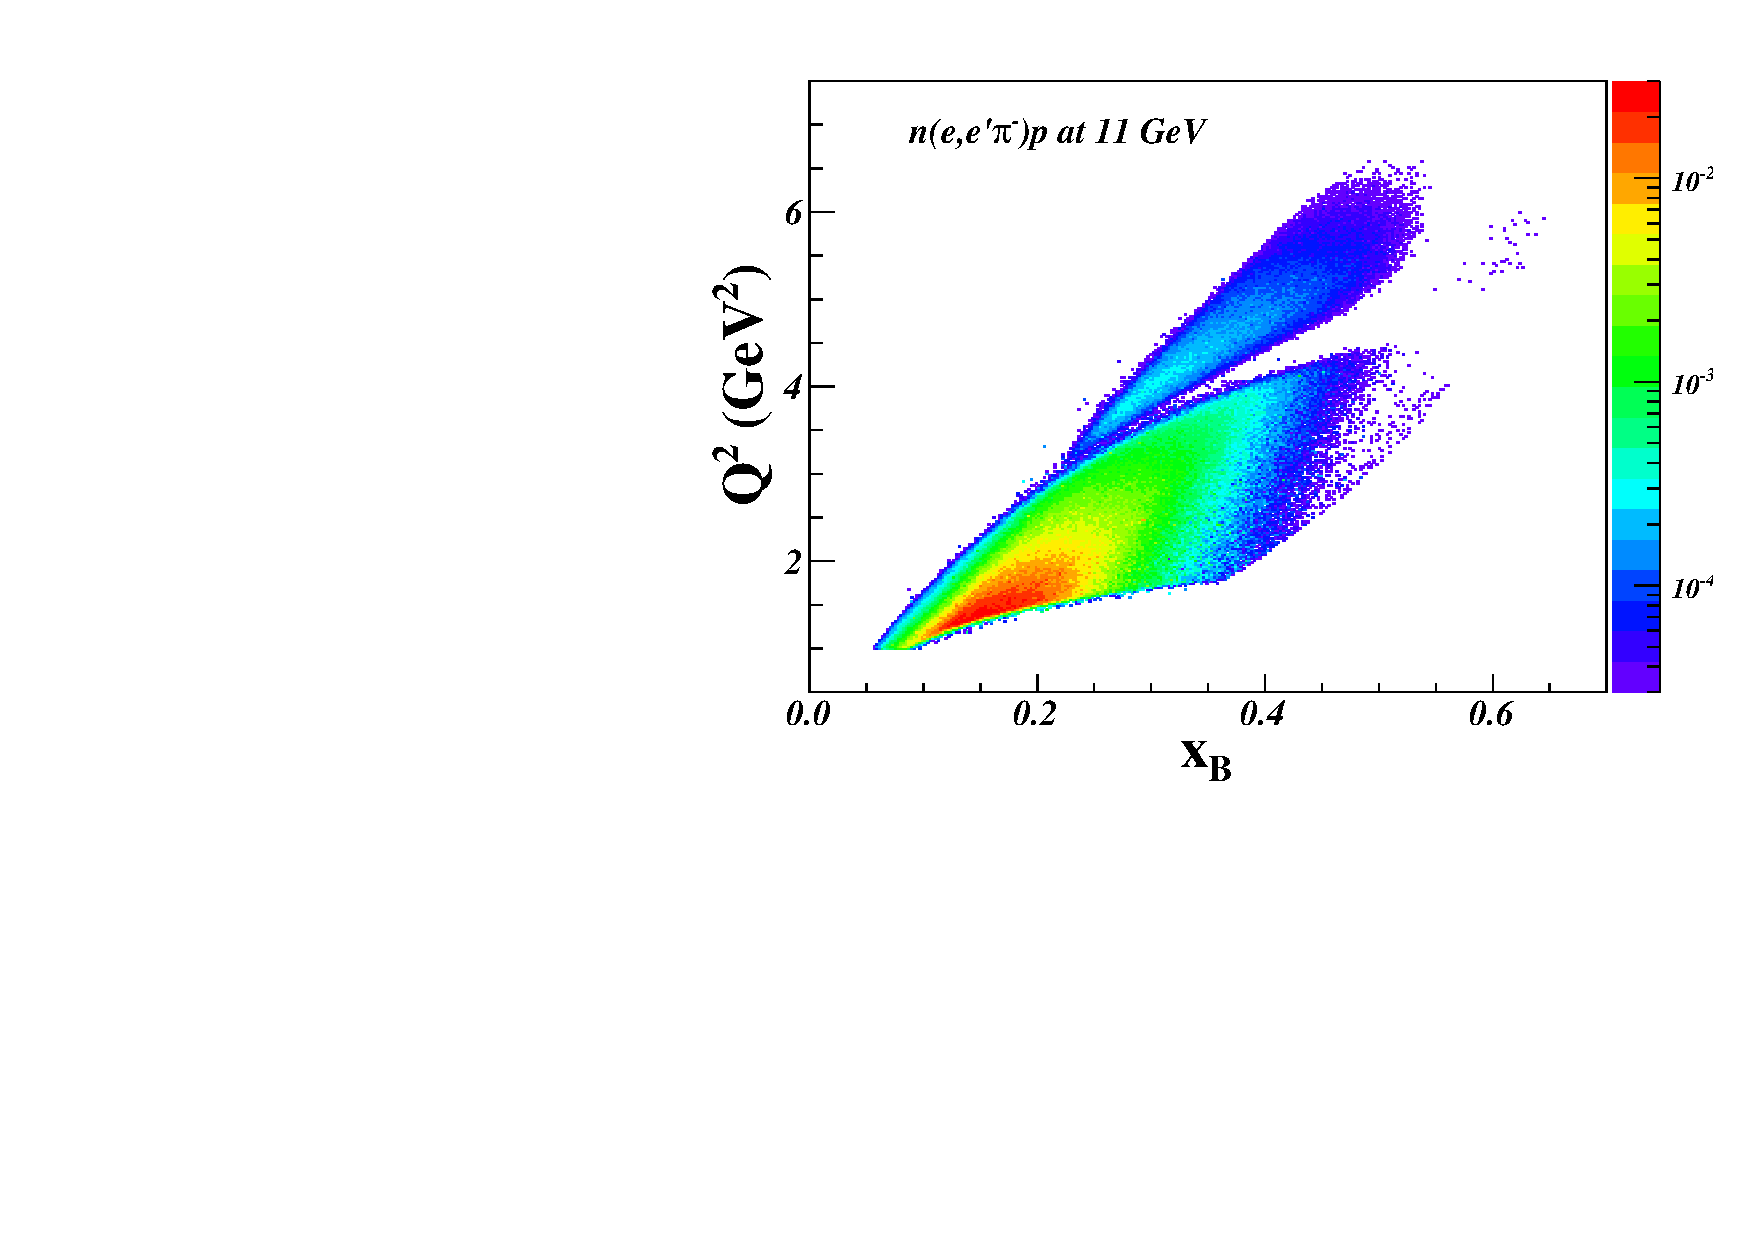
\includegraphics[type=pdf,
        ext=.pdf,read=.pdf,width=0.45\textwidth]{./figures/E11_Q2_x_prd_fermi}
           }
 \caption[The kinematic coverage at different acceptances.]{\footnotesize{The
     kinematic coverage at different acceptances at 11~GeV, when detecting all
recoil protons w/o (left) or w/ (right) an additional proton detector. Colors correspond to rates
(Hz) in log scale.}}
  \label{kin_cor_prd}
  \end{center}
\end{figure}
The kinematic coverage in $Q^{2}$ vs. $x_{B}$ is shown in Fig.~\ref{kin_cor_prd},
when adding a new proton recoil detector to detect the rest of the recoil
protons at larger angle ($24^{\circ}\sim50^{\circ}$), in addition to the existing SoLID detectors which cover the angle from  $8^{\circ}$ to $24^{\circ}$.


\begin{figure}[!ht]
 \begin{center}
     \subfloat[w/o PRD]{
	       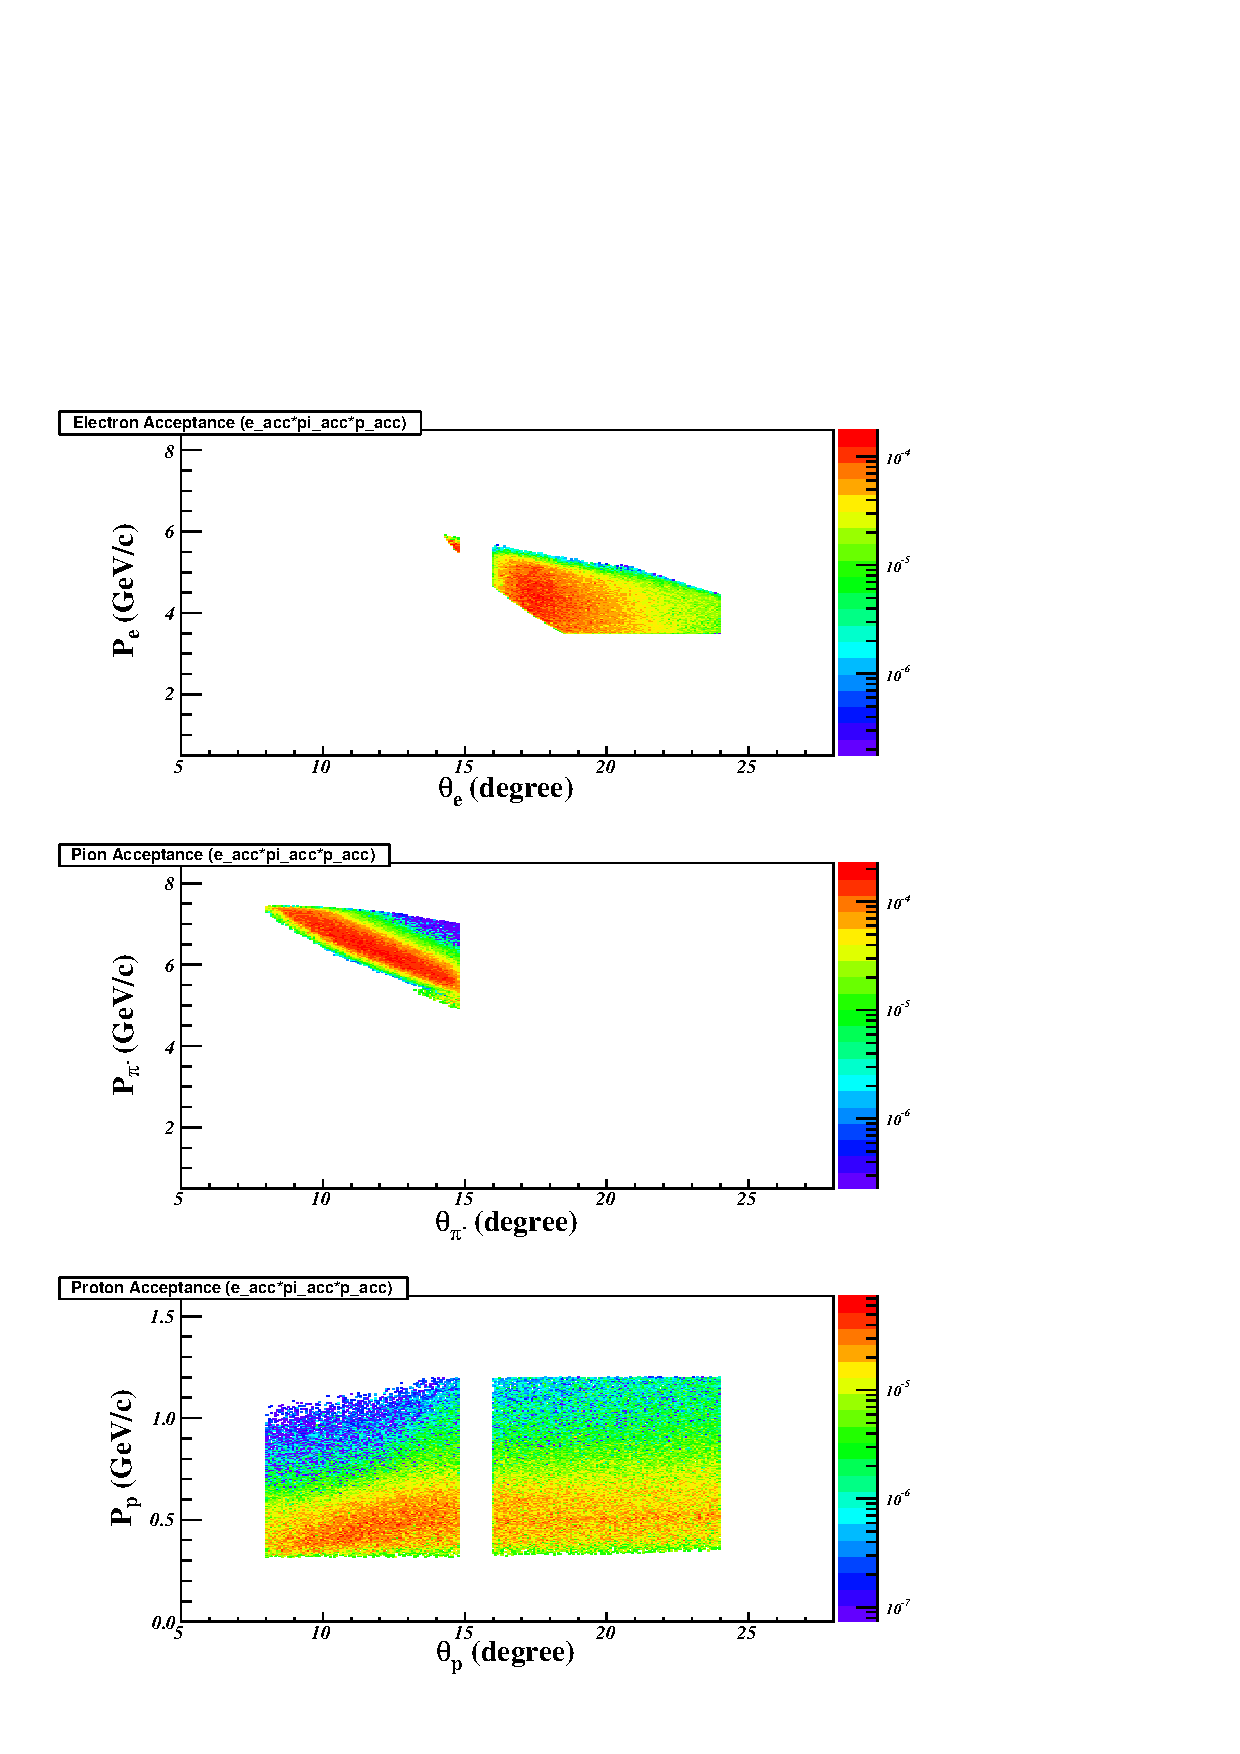
\includegraphics[type=pdf,
     ext=.pdf,read=.pdf,width=0.45\textwidth]{./figures/E11_acc_epip_Q2gt4}}
     \subfloat[w/ PRD]{
     ext=.pdf,read=.pdf,width=0.45\textwidth]{./figures/E11_acc_epi_Q2gt4}}
	 
  \caption[The acceptance of the momenta and scattering angles for electrons,
    $\pi^{-}$ and protons]{\footnotesize{The acceptance of the momenta and
    polar angles w/o (left) or w/ (right) the PRD. In each panel, he top, middle and
    bottom plots are for electrons, $\pi^{-}$ and protons, respectively. A
    cut of $Q^{2}>4~\mathrm{GeV^{2}}$ is applied. Colors correspond to rates
    (Hz) in log scale.}}
  \label{p_theta_prd}
  \end{center}
\end{figure}


\begin{table}[!ht]
\centering
\begin{tabular}{|c|c|c|}
 \hline
  1$<Q^2<$4~GeV$^2$ & $Q^2>$4~GeV$^2$ & Total\\
 \hline
\multicolumn{3}{|c|}{DEMP: $\vec{n}(e,e'\pi^{-}p)$ Triple-Coincidence (Hz)}\\
 \hline
 25.59 (6.11)   &  0.54 (0.26) & 26.13 (6.37)   \\
 \hline
\multicolumn{3}{|c|}{SIDIS: $\vec{n}(e,e'\pi^{-})X$ Double-Coincidence (Hz)}\\
 \hline
        1388.85 & 35.77        & 1424.62   \\
 \hline
\end{tabular}
\caption[Triple-Coincidence rates for
  neutron-DEMP]{\footnotesize{Triple-Coincidence rates for DEMP events compared
    with the SIDIS rates. Numbers in brackets are the DEMP rates with only
    detecting protons using only the SoLID detectors. The online production
    trigger will be the SIDIS double-coincidence trigger of which rates are
    also given.}}
\label{rate_table_prd}
\end{table} 



\begin{figure}[!ht]
 \begin{center}
       \subfloat[w/o PRD]{
      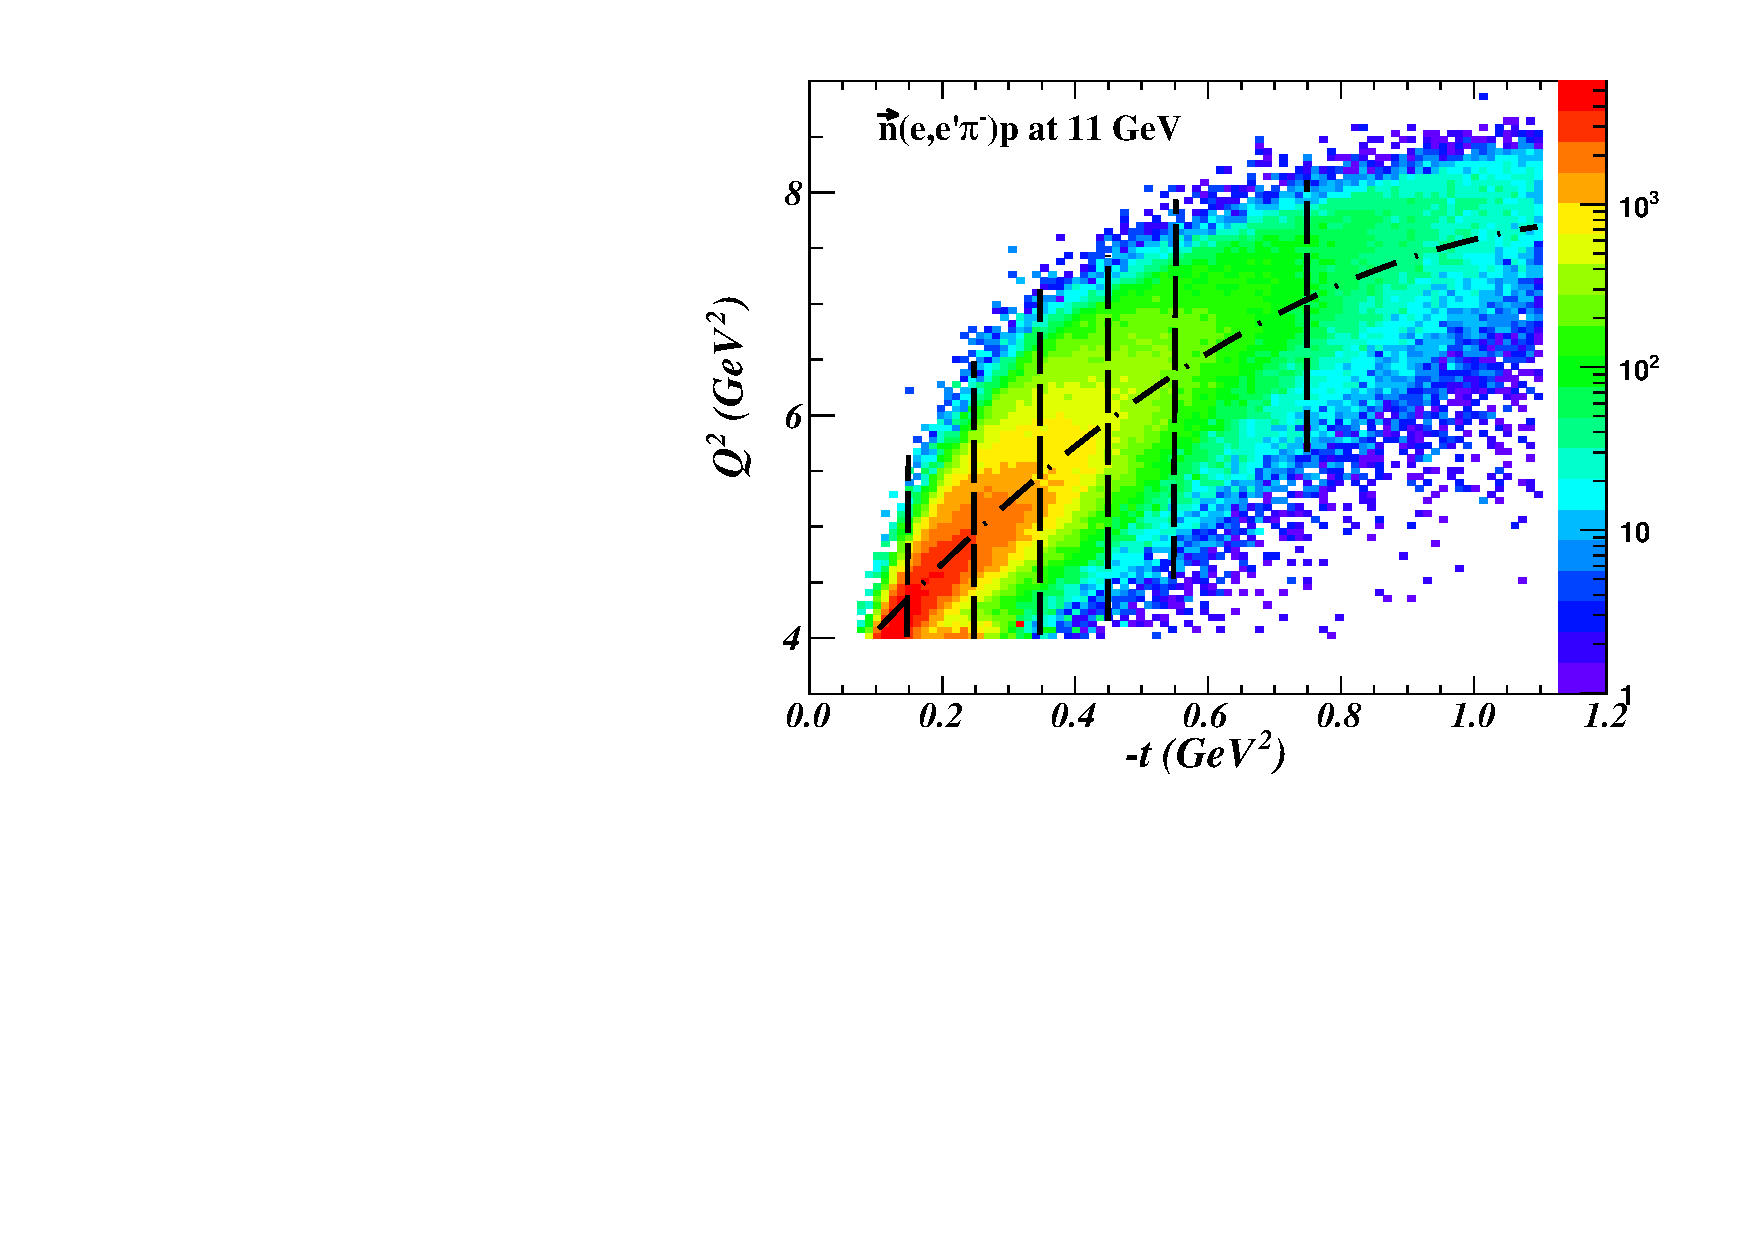
\includegraphics[type=pdf,
        ext=.pdf,read=.pdf,width=0.5\textwidth]{./figures/E11_Q2_t_bin_Fermi} }
        \subfloat[w/ PRD]{
      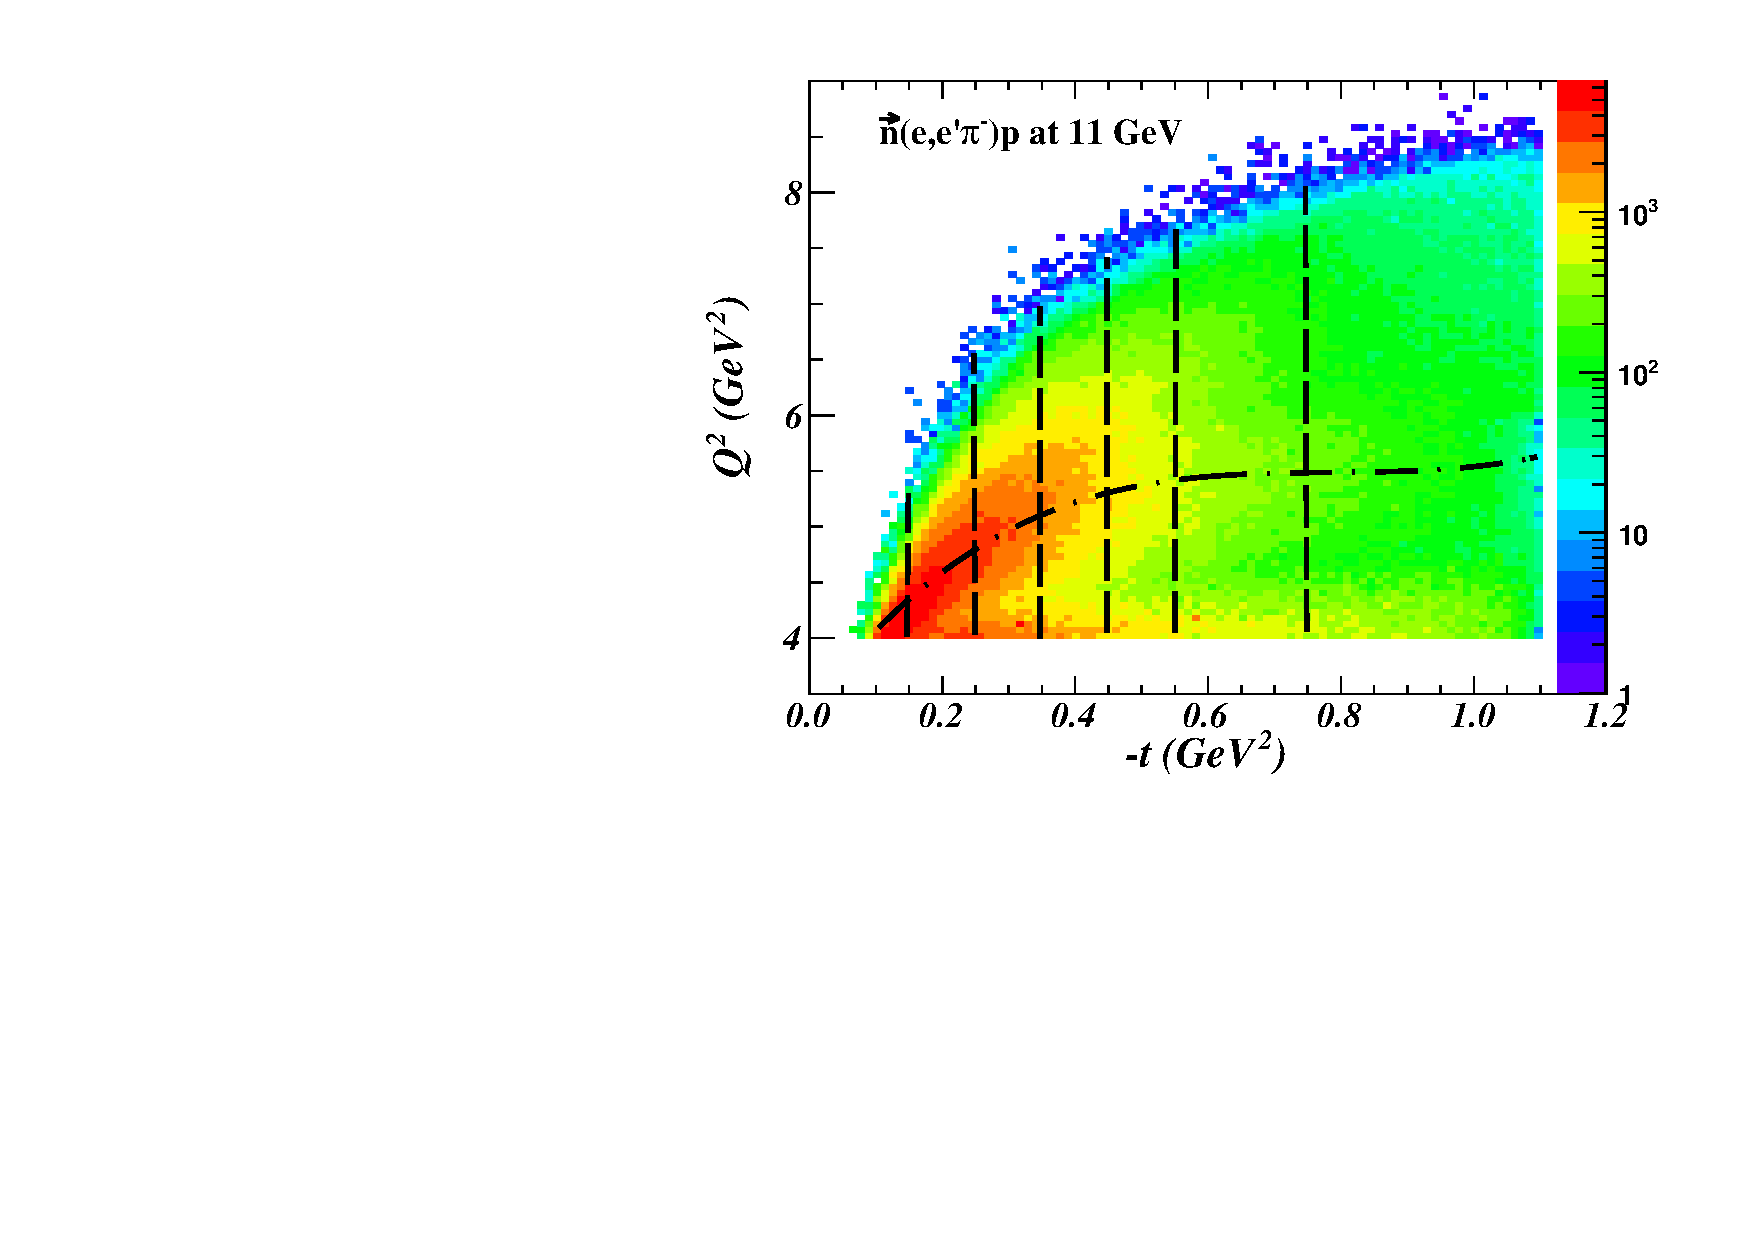
\includegraphics[type=pdf,
        ext=.pdf,read=.pdf,width=0.5\textwidth]{./figures/E11_Q2_t_bin_prd_Fermi} }
   \caption[$Q^{2}$ vs. $-t$]{\footnotesize{$Q^{2}$ vs. $-t$ where the black
dash lines specify the boundaries of 7 $-t$ bins and the black dash-dot lines
indicate the additional two $Q^{2}$ bins.  The color panel indicates the raw
counts with 48 days of beam time at 11~GeV.}}
  \label{Q2_t_bin_prd}
  \end{center}
\end{figure}

\begin{figure}[!ht]
 \begin{center}
         \subfloat[w/o PRD]{
               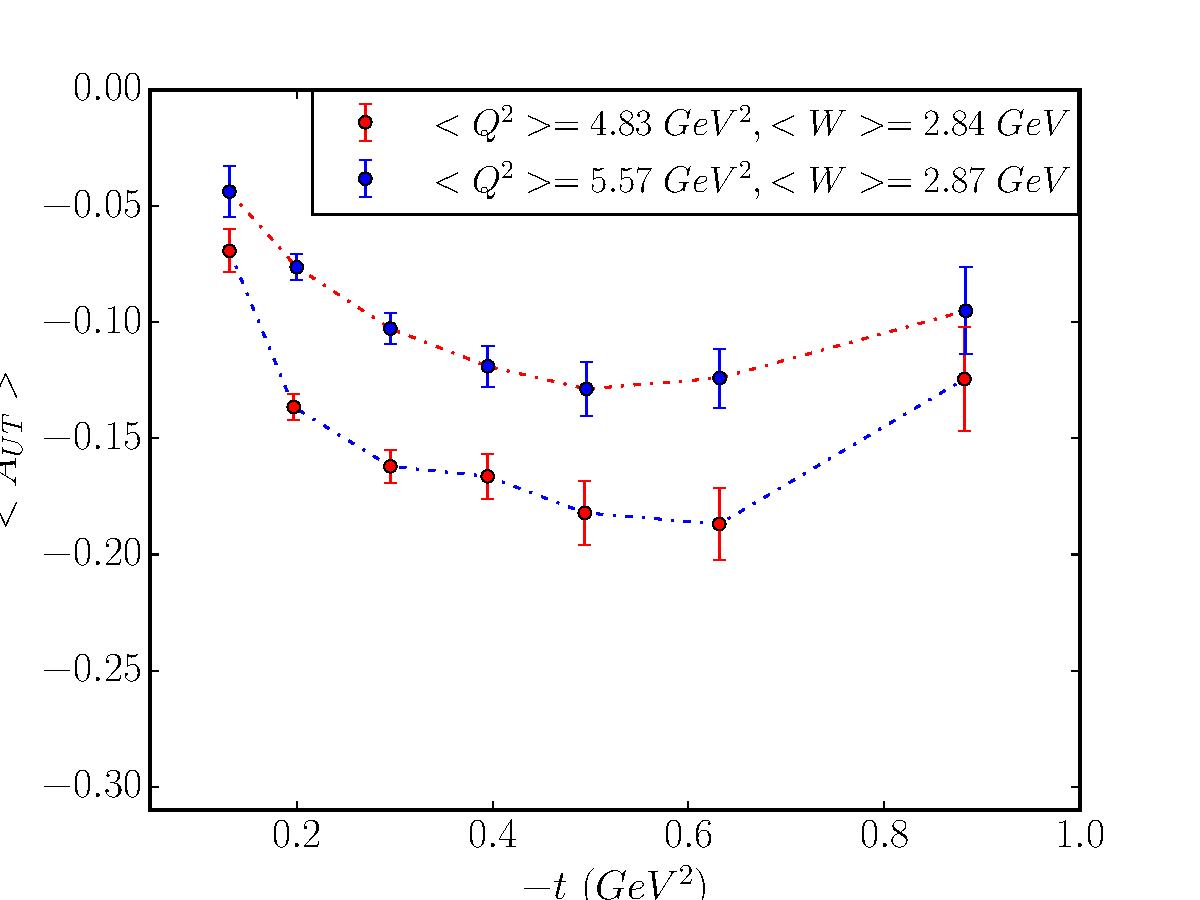
\includegraphics[type=pdf,
        ext=.pdf,read=.pdf,width=0.45\textwidth]{./figures/bin_asym_t_fermi} }
            \subfloat[w/ PRD]{
      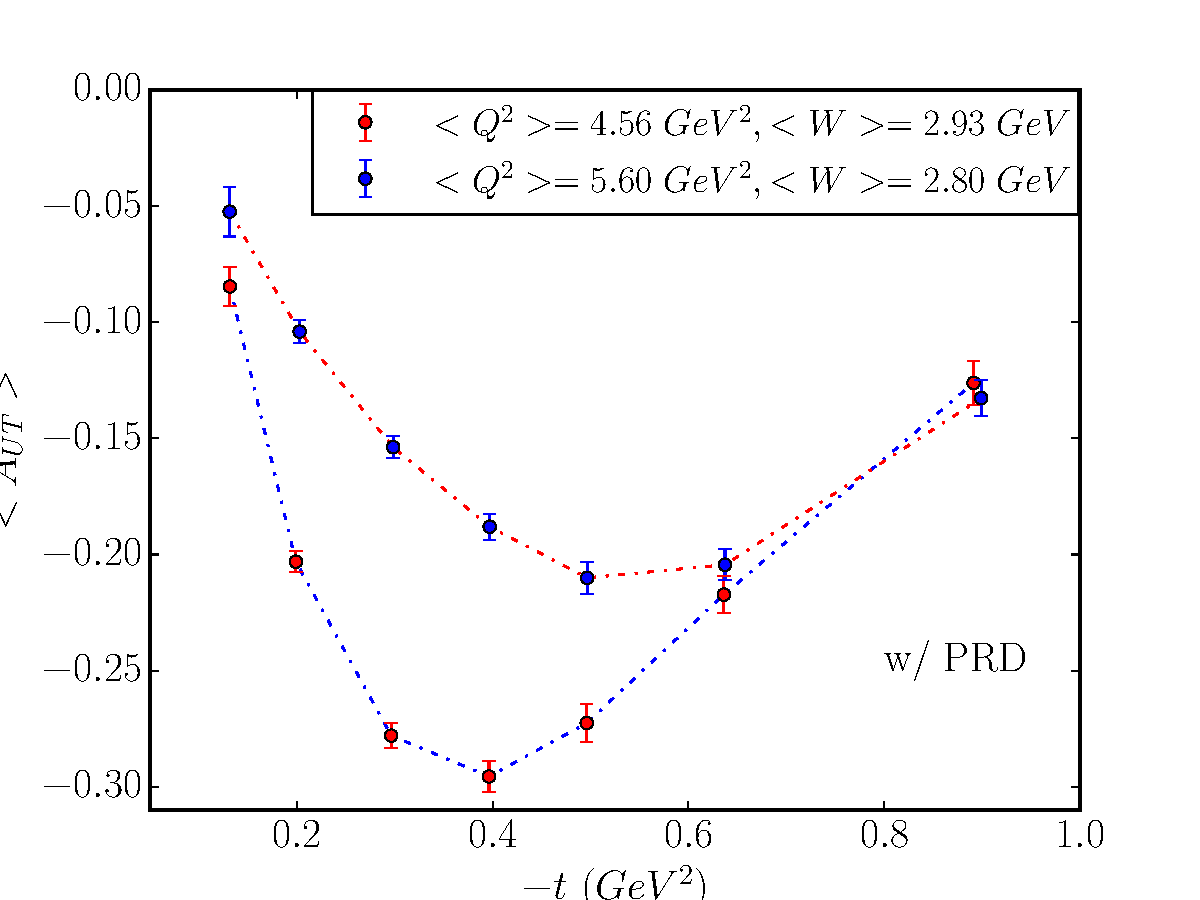
\includegraphics[type=pdf,
        ext=.pdf,read=.pdf,width=0.45\textwidth]{./figures/bin_asym_t_prd_fermi} }
      \caption{\footnotesize{Projection of target single spin asymmetry
          ($A_{UT}$) as a function of $-t$ for DEMP with transversely polarized
          $\mathrm{^{3}He}$ at $E_{0}$=11~GeV (directly compare with
Fig.~\ref{fig:hermes_aut}).  The data in each $-t$ bin are further divided into
two $Q^{2}$ bins with similar statistics.  The error bars are the projected
statistical uncertainties defined in Eq.~\ref{stat_err}. The asymmetry value in
each bin is predicted with the model given in Appendix-A and is diluted due to
not separating the L/T contributions. The left plot shows the projection w/o a
new proton recoil detector, while the right plot shows a better projected
result with a new detector in addition. One can see the average asymmetries are
also changed between two configurations because the asymmetry dilution
strongly depends on $Q^{2}$, which changes w/ or w/o the PRD.}}
  \label{asym_t}
  \end{center}
\end{figure}


\begin{table}[!ht]
\centering
 \small
\begin{tabular}{|c|c|c|c|c|c|c|c|}
\multicolumn{8}{c}{ (a) w/o PRD} \\
\hline
       &  t-bin\#1 & t-bin\#2 & t-bin\#3 & t-bin\#4 & t-bin\#5 & t-bin\#6 & t-bin\#7 \\
\hline $<-t>$ &  0.13 &  0.20 & 0.30 & 0.39 & 0.49 & 0.63 & 0.88 \\
\hline
\multicolumn{8}{|c|}{$Q^{2}$ bin-set\#1 } \\
\hline
$<Q^{2}>$      &  4.13 &  4.42 & 4.90 & 5.35 & 5.76 & 6.23 & 6.86 \\
$<\sigma_{L}/\sigma_{T}>$   &  6.43 &  5.13 & 3.90 & 3.09 & 2.43 & 1.65 & 0.69 \\
$<f_{L/T}>$    &  0.80 &  0.77 & 0.73 & 0.68 & 0.62 & 0.52 & 0.30 \\
$<A_{UT}>$     &  -6.93$\times 10^{-2}$ &  -1.36$\times 10^{-1}$ & -1.62$\times 10^{-1}$ &
 -1.66$\times 10^{-1}$ & -1.82$\times 10^{-1}$ & -1.87$\times 10^{-1}$ & -1.24$\times 10^{-1}$ \\               
$\delta A_{UT}$&  9.23$\times 10^{-3}$ &  5.62$\times 10^{-3}$ & 7.16$\times 10^{-3}$ & 
9.72$\times 10^{-3}$ & 1.39$\times 10^{-2}$ & 1.54$\times 10^{-2}$ &  2.24$\times 10^{-2}$ \\
$N$           &  3.26$\times 10^{4}$ &  8.73$\times 10^{4}$ & 5.37$\times 10^{4}$ 
& 2.91$\times 10^{4}$ & 1.42$\times 10^{4}$ & 1.15$\times 10^{4}$ & 5.50$\times 10^{3}$ \\
\hline
\multicolumn{8}{|c|}{$Q^{2}$ bin-set\#2 } \\
\hline 
$<Q^{2}>$     &  4.39 &  4.93 & 5.58 & 6.13 & 6.59 & 7.09 & 7.73 \\
$<\sigma_{L}/\sigma_{T}>$&  7.19 &  6.38 & 5.51 & 4.63 & 3.70 & 2.57 & 1.21 \\
$<f_{L/T}>$   &  0.81 &  0.80 & 0.78 & 0.74 & 0.70 & 0.61 & 0.42 \\
$<A_{UT}>$    &  -4.38$\times 10^{-2}$ &  -7.63$\times 10^{-2}$ & -1.03$\times 10^{-1}$ & 
-1.19$\times 10^{-1}$ & -1.29$\times 10^{-1}$ & -1.24$\times 10^{-1}$ & -9.51$\times 10^{-2}$ \\
$\delta A_{UT}$&  1.13$\times 10^{-2}$ &  5.82$\times 10^{-3}$ & 6.83$\times 10^{-3}$ 
& 9.05$\times 10^{-3}$ & 1.21$\times 10^{-2}$ & 1.32$\times 10^{-2}$ & 1.94$\times 10^{-2}$ \\
$N$          &  2.17$\times 10^{4}$ &  8.19$\times 10^{4}$ & 5.94$\times 10^{4}$ &
  3.38$\times 10^{4}$ & 1.88$\times 10^{4}$ & 1.59$\times 10^{4}$ & 7.32$\times 10^{3}$ \\
\hline
\multicolumn{8}{c}{} \\
\multicolumn{8}{c}{ (b) w/ PRD} \\
\hline
	     &  t-bin\#1 & t-bin\#2 & t-bin\#3 & t-bin\#4 & t-bin\#5 & t-bin\#6 & t-bin\#7 \\
\hline 
$<-t>$       &  0.13 & 0.20   & 0.30   & 0.40   & 0.50   & 0.64   & 0.90  \\
\hline
\multicolumn{8}{|c|}{$Q^{2}$ bin-set\#1 } \\
\hline
$<Q^{2}>$   &  4.12 &  4.34 & 4.59 & 4.74 & 4.83 & 4.86 & 4.84 \\
$<\sigma_{L}/\sigma_{T}>$&  6.41 &  4.90 & 3.37 & 2.32 & 1.62 & 1.02 & 0.46 \\
$<f_{L/T}>$   &  0.80 &  0.76 & 0.69 & 0.60 & 0.52 & 0.40 & 0.23 \\
$<A_{UT}>$ &  -8.46$\times 10^{-2}$ &  -2.03$\times 10^{-1}$ & -2.78$\times 10^{-1}$ & 
-2.96$\times 10^{-1}$ & -2.73$\times 10^{-1}$ & -2.17$\times 10^{-1}$ & -1.26$\times 10^{-1}$ \\
$\delta A_{UT}$&  8.57$\times 10^{-3}$ &  4.58$\times 10^{-3}$ & 5.30$\times 10^{-3}$ & 
6.58$\times 10^{-3}$ & 8.24$\times 10^{-3}$ & 7.97$\times 10^{-3}$ & 9.57$\times 10^{-3}$ \\
$N$     &  3.77$\times 10^{4}$ &  1.31$\times 10^{5}$ & 9.61$\times 10^{4}$ &
6.22$\times 10^{4}$ & 3.98$\times 10^{4}$ & 4.30$\times 10^{4}$ & 3.02$\times 10^{4}$ \\   
\hline
\multicolumn{8}{|c|}{$Q^{2}$ bin-set\#2 } \\
\hline 
$<Q^{2}>$   &  4.40 &  4.88 & 5.39 & 5.77 & 6.07 & 6.35 & 6.66 \\
$<\sigma_{L}/\sigma_{T}>$   &  7.19 &  6.15 & 4.96 & 3.84 & 2.88 & 1.81 & 0.69 \\
$<f_{L/T}>$  &  0.81 &  0.79 & 0.76 & 0.71 & 0.65 & 0.53 & 0.30 \\
$<A_{UT}>$   &  -5.24$\times 10^{-2}$ &  -1.04$\times 10^{-1}$ & -1.54$\times 10^{-1}$ 
& -1.88$\times 10^{-1}$ & -2.10$\times 10^{-1}$ & -2.04$\times 10^{-1}$ & -1.33$\times 10^{-1}$ \\
$\delta A_{UT}$&  1.07$\times 10^{-2}$ &  4.86$\times 10^{-3}$ & 4.86$\times 10^{-3}$ & 
5.57$\times 10^{-3}$ & 6.88$\times 10^{-3}$ & 6.62$\times 10^{-3}$ & 7.64$\times 10^{-3}$ \\
$N$         &  2.42$\times 10^{4}$ &  1.17$\times 10^{5}$ & 1.17$\times 10^{5}$& 8.85$\times 10^{4}$ 
& 5.78$\times 10^{4}$ & 6.24$\times 10^{4}$ & 4.73$\times 10^{4}$ \\
\hline
\end{tabular}
\caption[Detailed information of projected bins]{\footnotesize{Detailed
information of projected bins from the new DEMP measurements with SoLID, while
$<Q^{2}>$ and $<-t>$ are in the unit of GeV$^{2}$. The top (bottom) table is
with respect to the case of proton detection w/o (w/) a new PRD. The data are
divided into 14 $-t$ bins in both $-t$ (7 bins) and $Q^{2}$ (2 bins).}}
\label{asym_bin_table_prd}
\end{table} 


\section(Improvement to the Missing Mass and Background Rejection)

\begin{figure}[!ht]
\begin{center}
\subfloat[w/o PRD]{
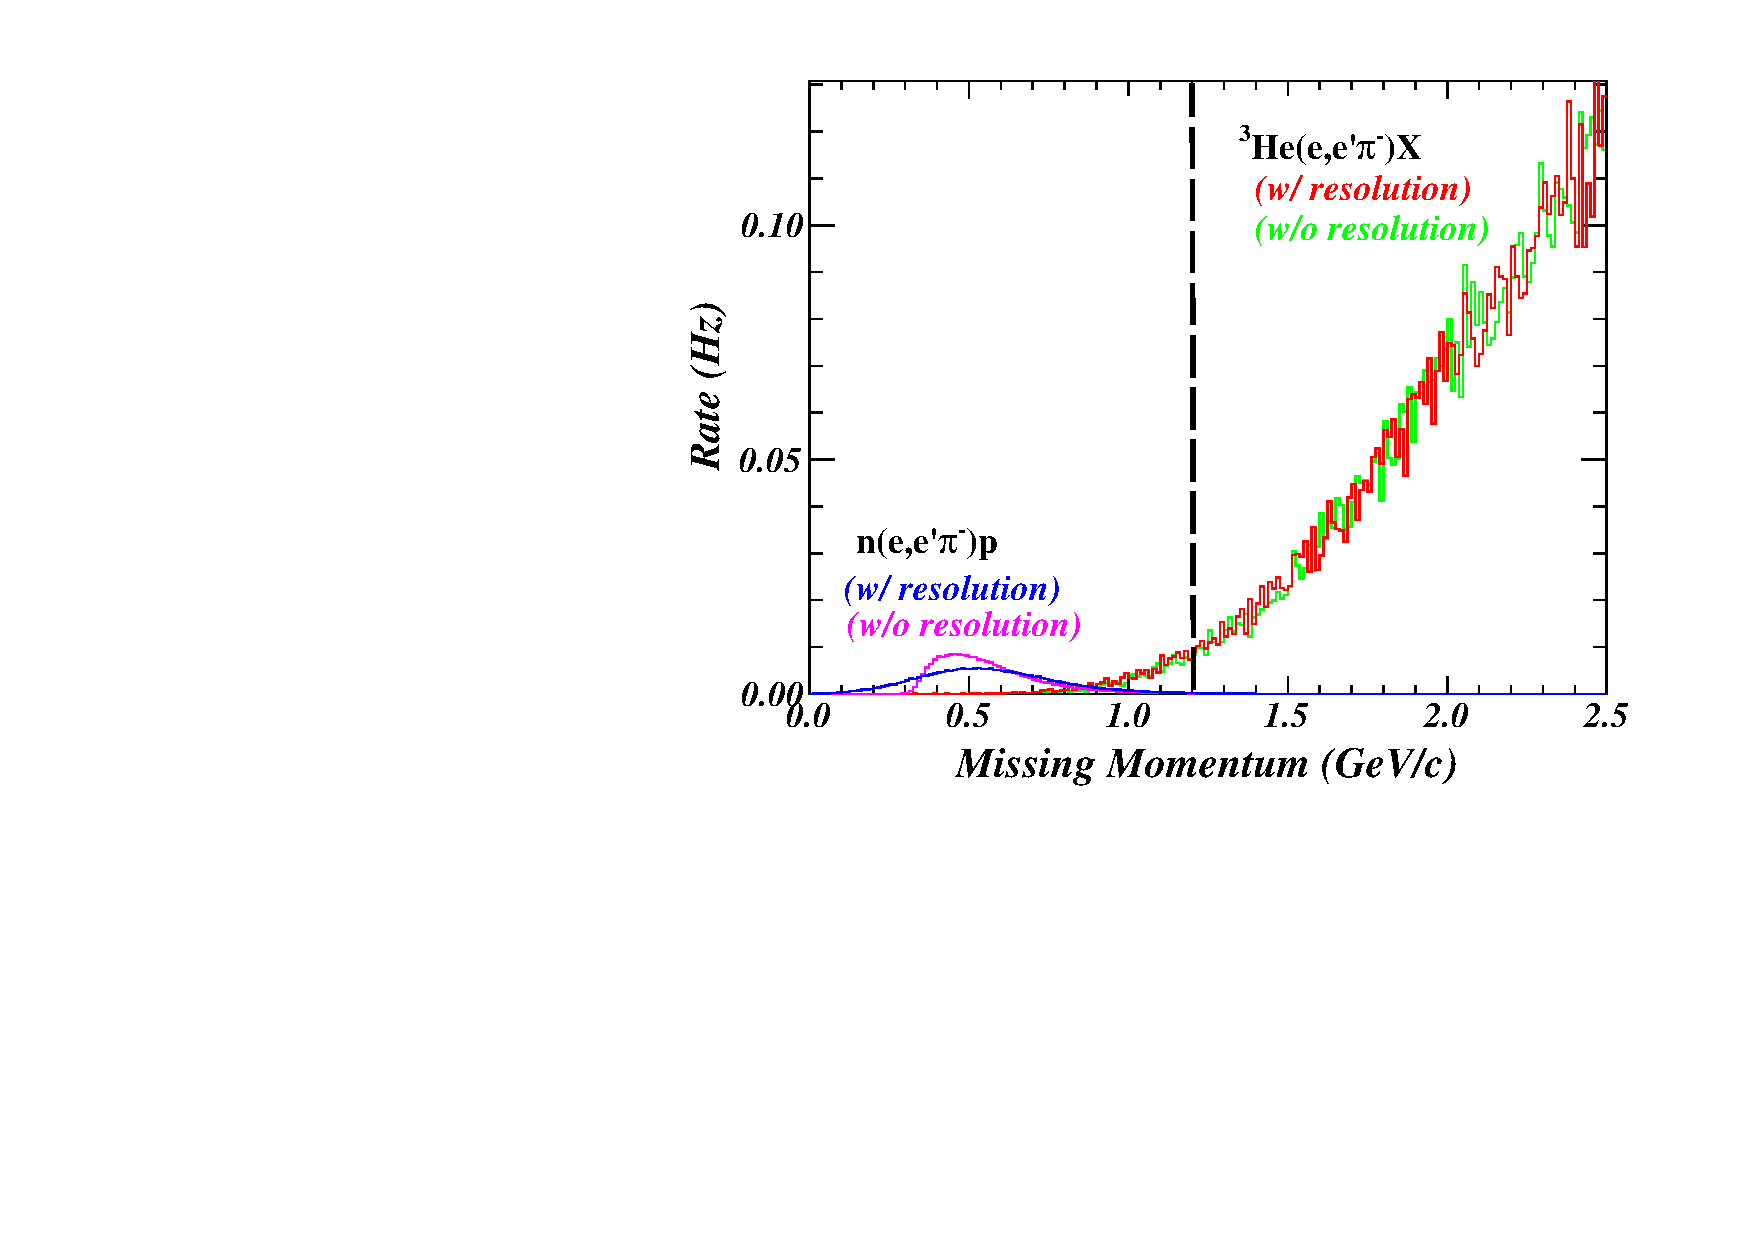
\includegraphics[type=pdf,ext=.pdf,read=.pdf,width=0.5\textwidth]{./figures/Missing_P_Fermi}}
\subfloat[w/ PRD]{
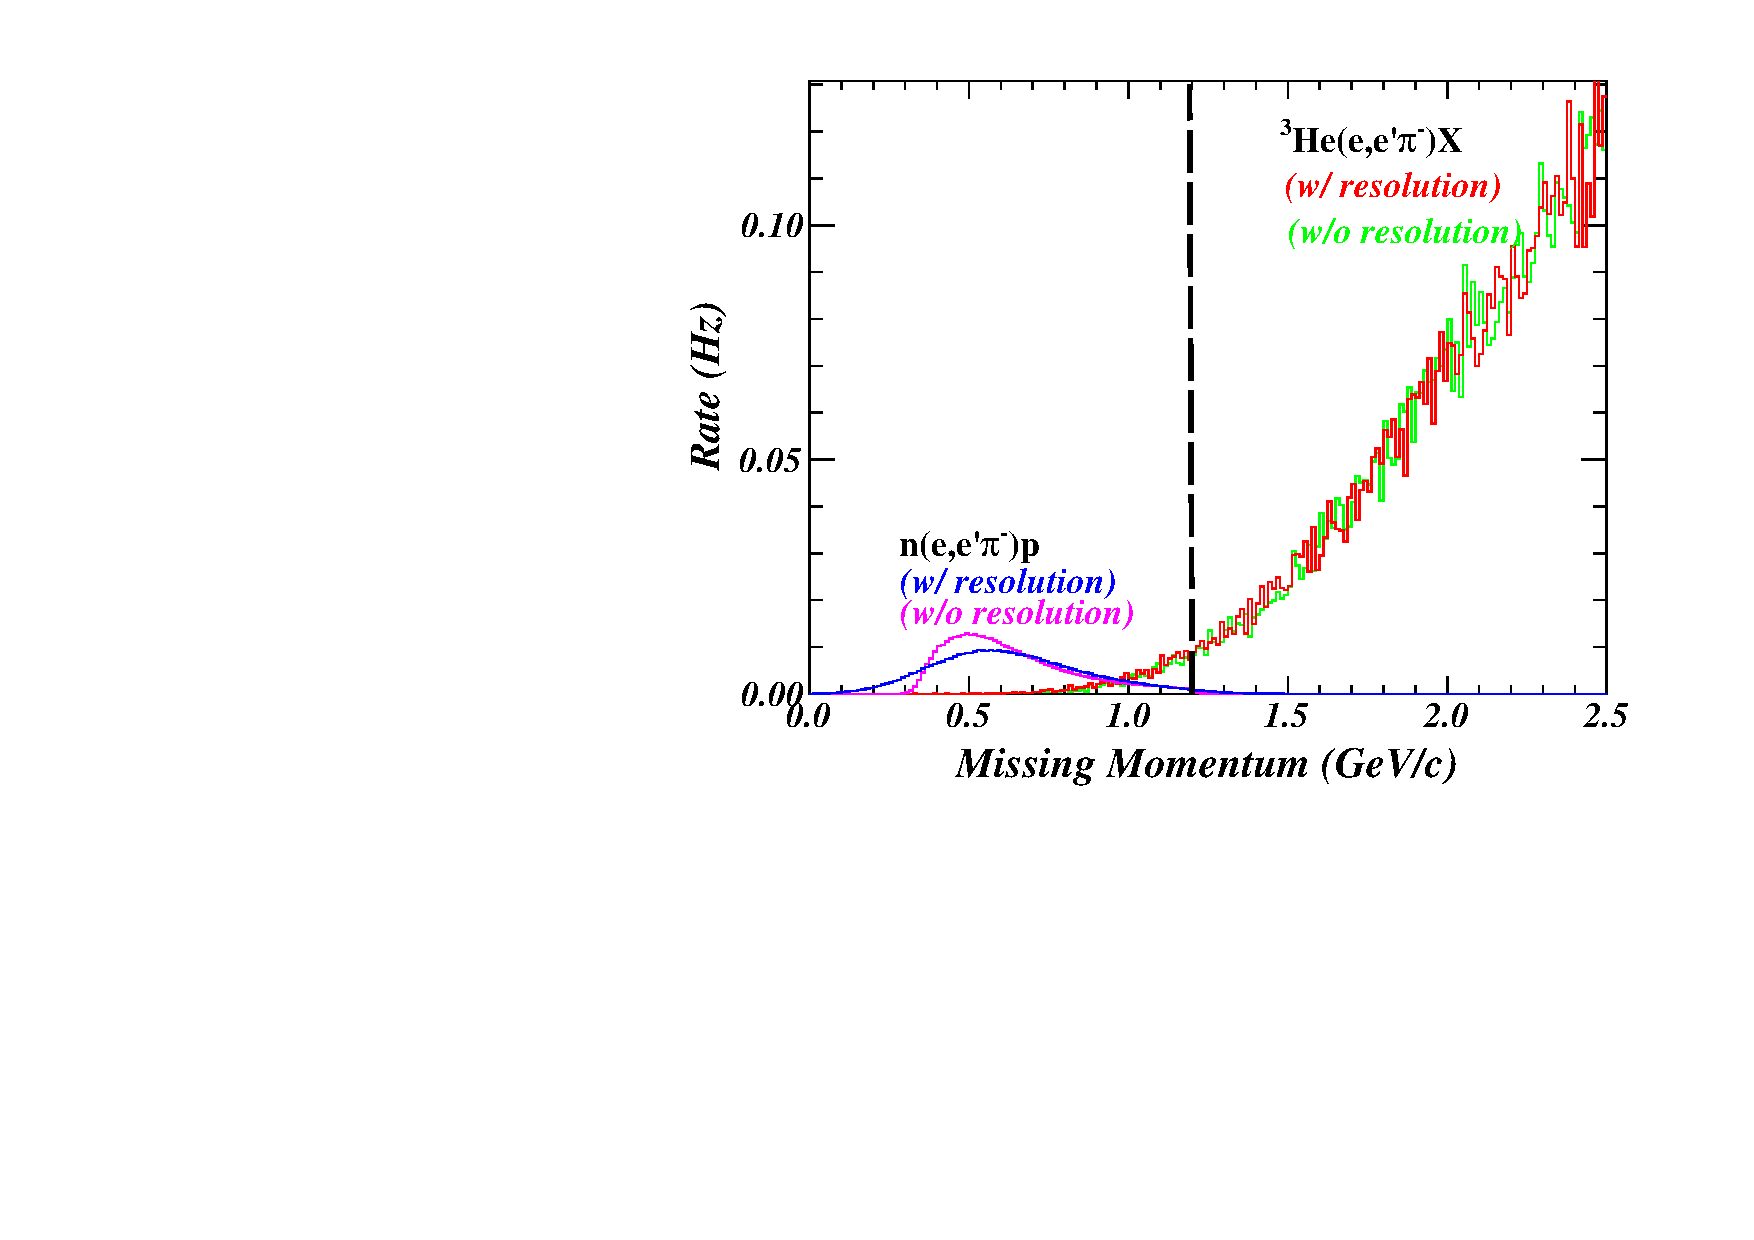
\includegraphics[type=pdf,ext=.pdf,read=.pdf,width=0.5\textwidth]{./figures/Missing_P_PRD_Fermi}} 
\caption[Missing Momentum]{\footnotesize{Missing momentum spectra of DEMP
and SIDIS events. The missing momentum distributions are well separated between
the two processes and one can apply a cut at $P_{miss}<1.2$~GeV/c (indicated by the
black dashed line) to remove most of the SIDIS events.}}
  \label{missing_mom_prd}
  \end{center}
\end{figure}

\begin{figure}[!ht]
 \begin{center}
       \subfloat[w/o PRD]{
      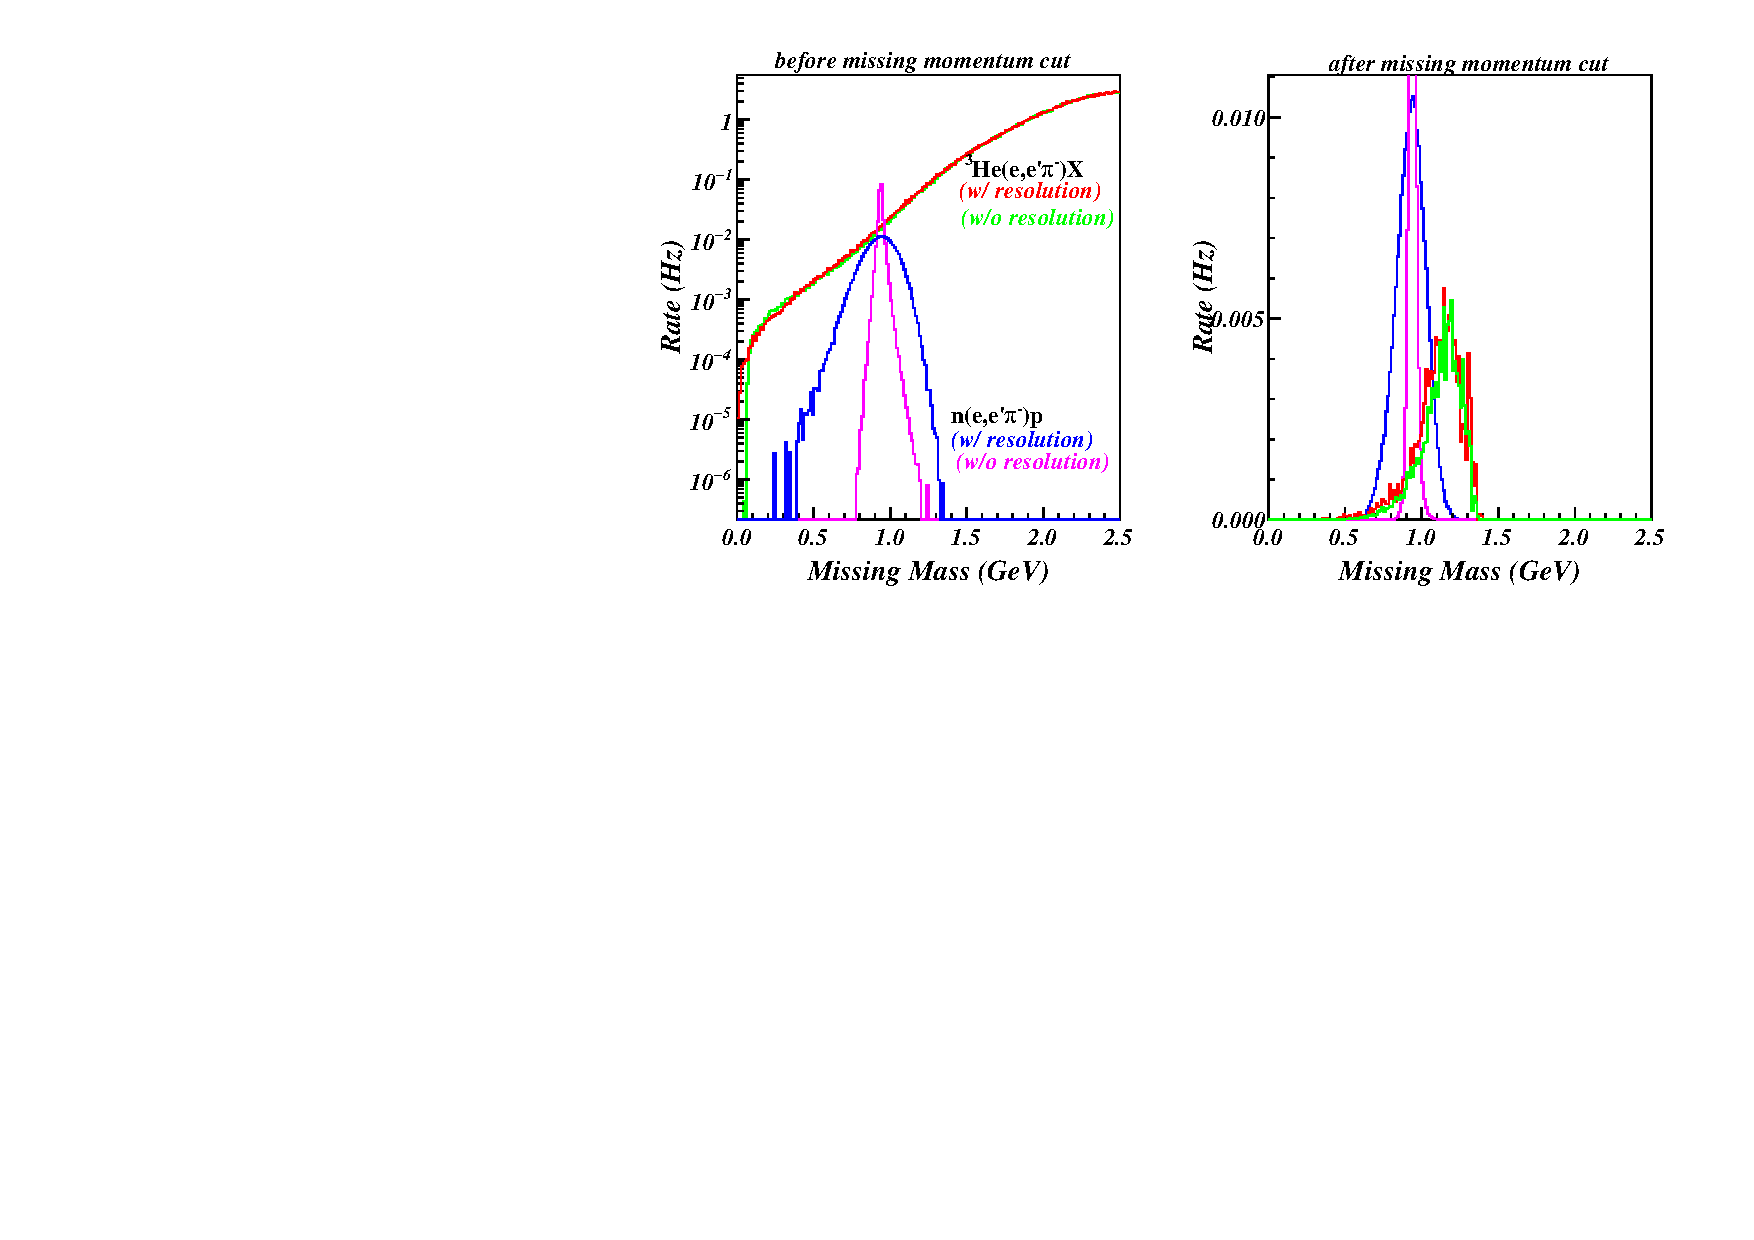
\includegraphics[type=pdf,
        ext=.pdf,read=.pdf,width=0.85\textwidth]{./figures/Missing_Mass_Fermi} }\\
          \subfloat[w/ PRD]{
      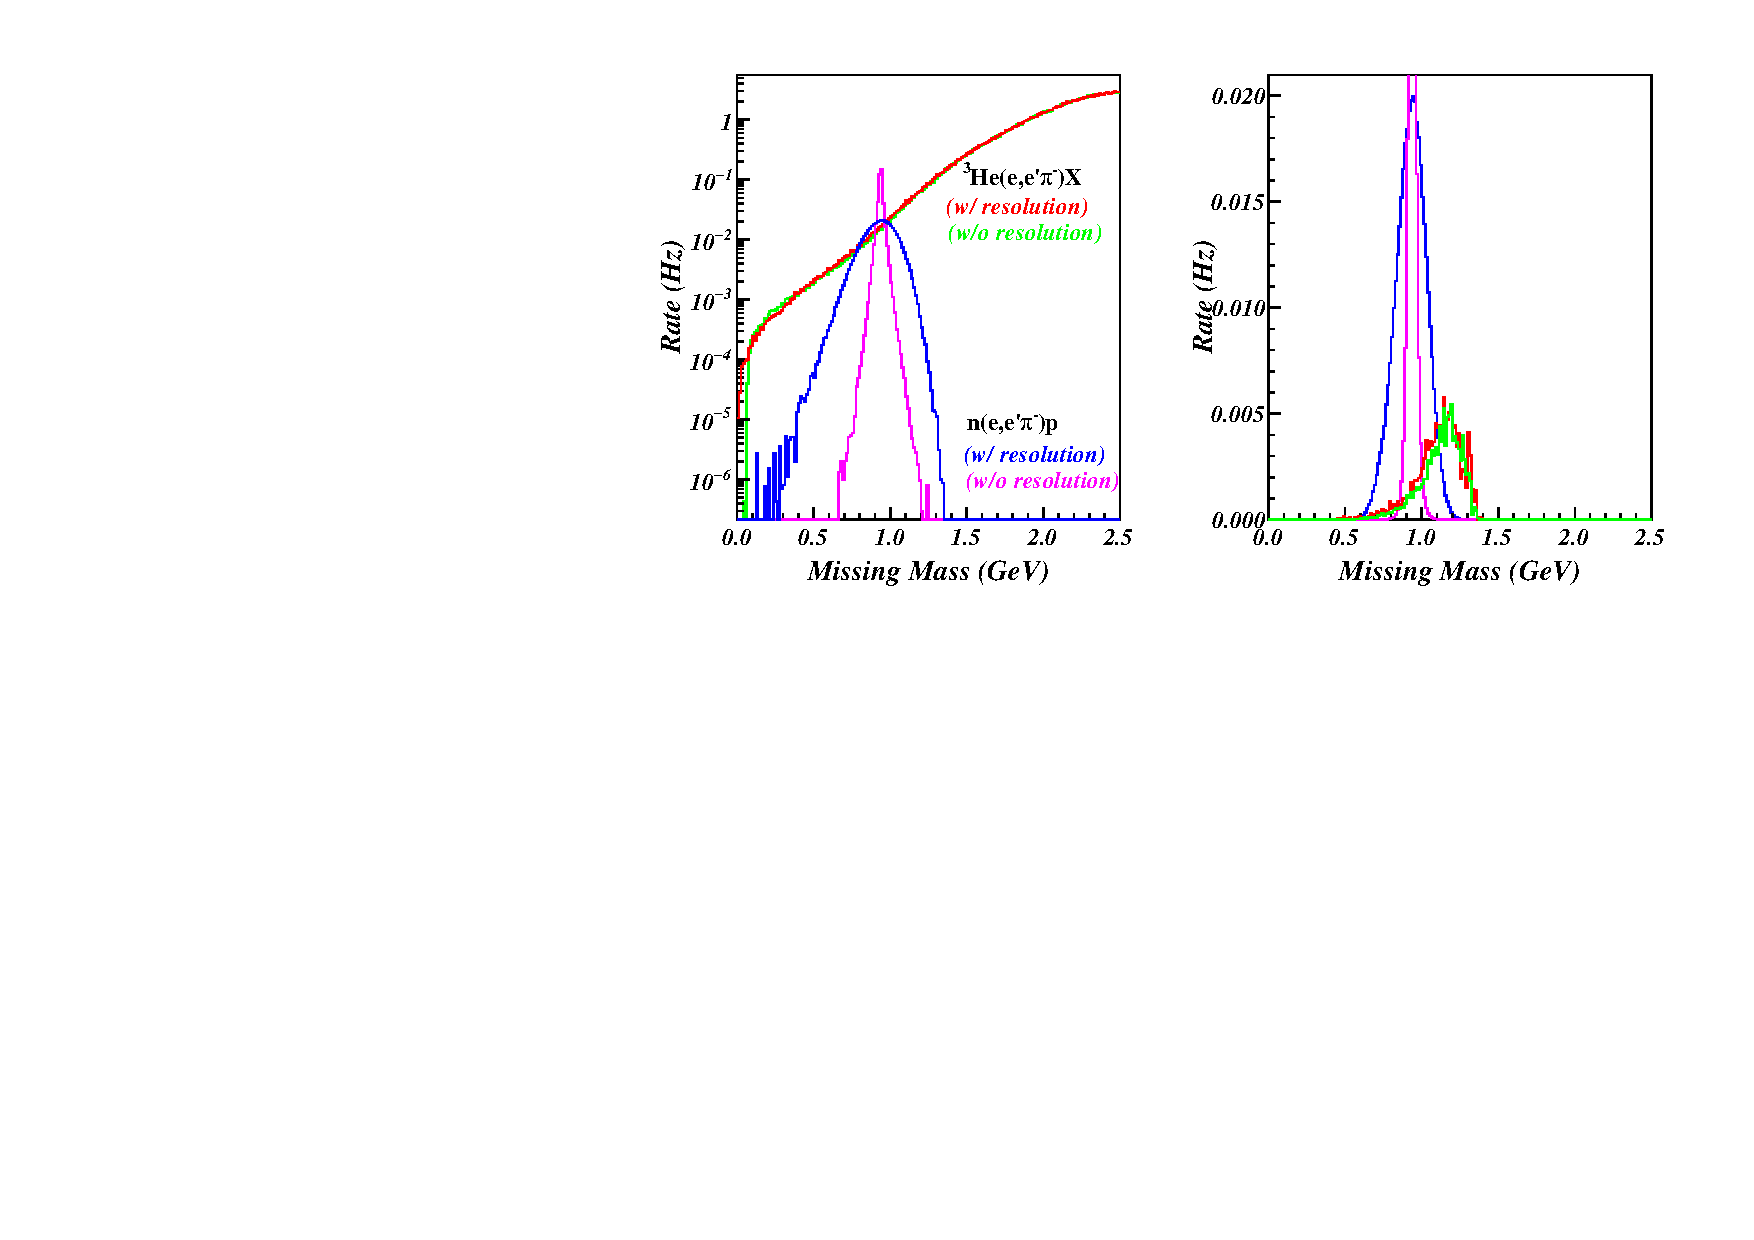
\includegraphics[type=pdf,
        ext=.pdf,read=.pdf,width=0.85\textwidth]{./figures/Missing_Mass_PRD_Fermi} } 
   \caption[Missing Mass]{\footnotesize{Missing mass spectra of DEMP and SIDIS
events. Top (bottom) panel shows the missing mass distribution of DEMP events
w/o (w/) proton detection by a new PRD.  The left (right) plot of each panel 
shows the background contamination from SIDIS events before (after) the
missing momentum cut shown in Fig.~\ref{missing_mom}. The broadening effect of
the missing mass due to only the Fermi motion is indicated by the magenta
curve. The SIDIS background is already small compared with DEMP events before
optimizing the cut. The actual SIDIS background should be much smaller, since
we overestimated the SIDIS rate by assuming all target fragments ("X") in the
SIDIS process contain protons.}}
  \label{missing_mass_prd}
  \end{center}
\end{figure}


\section{Requirements and Conceptual Design}

\begin{figure}[!ht]
 \begin{center}
  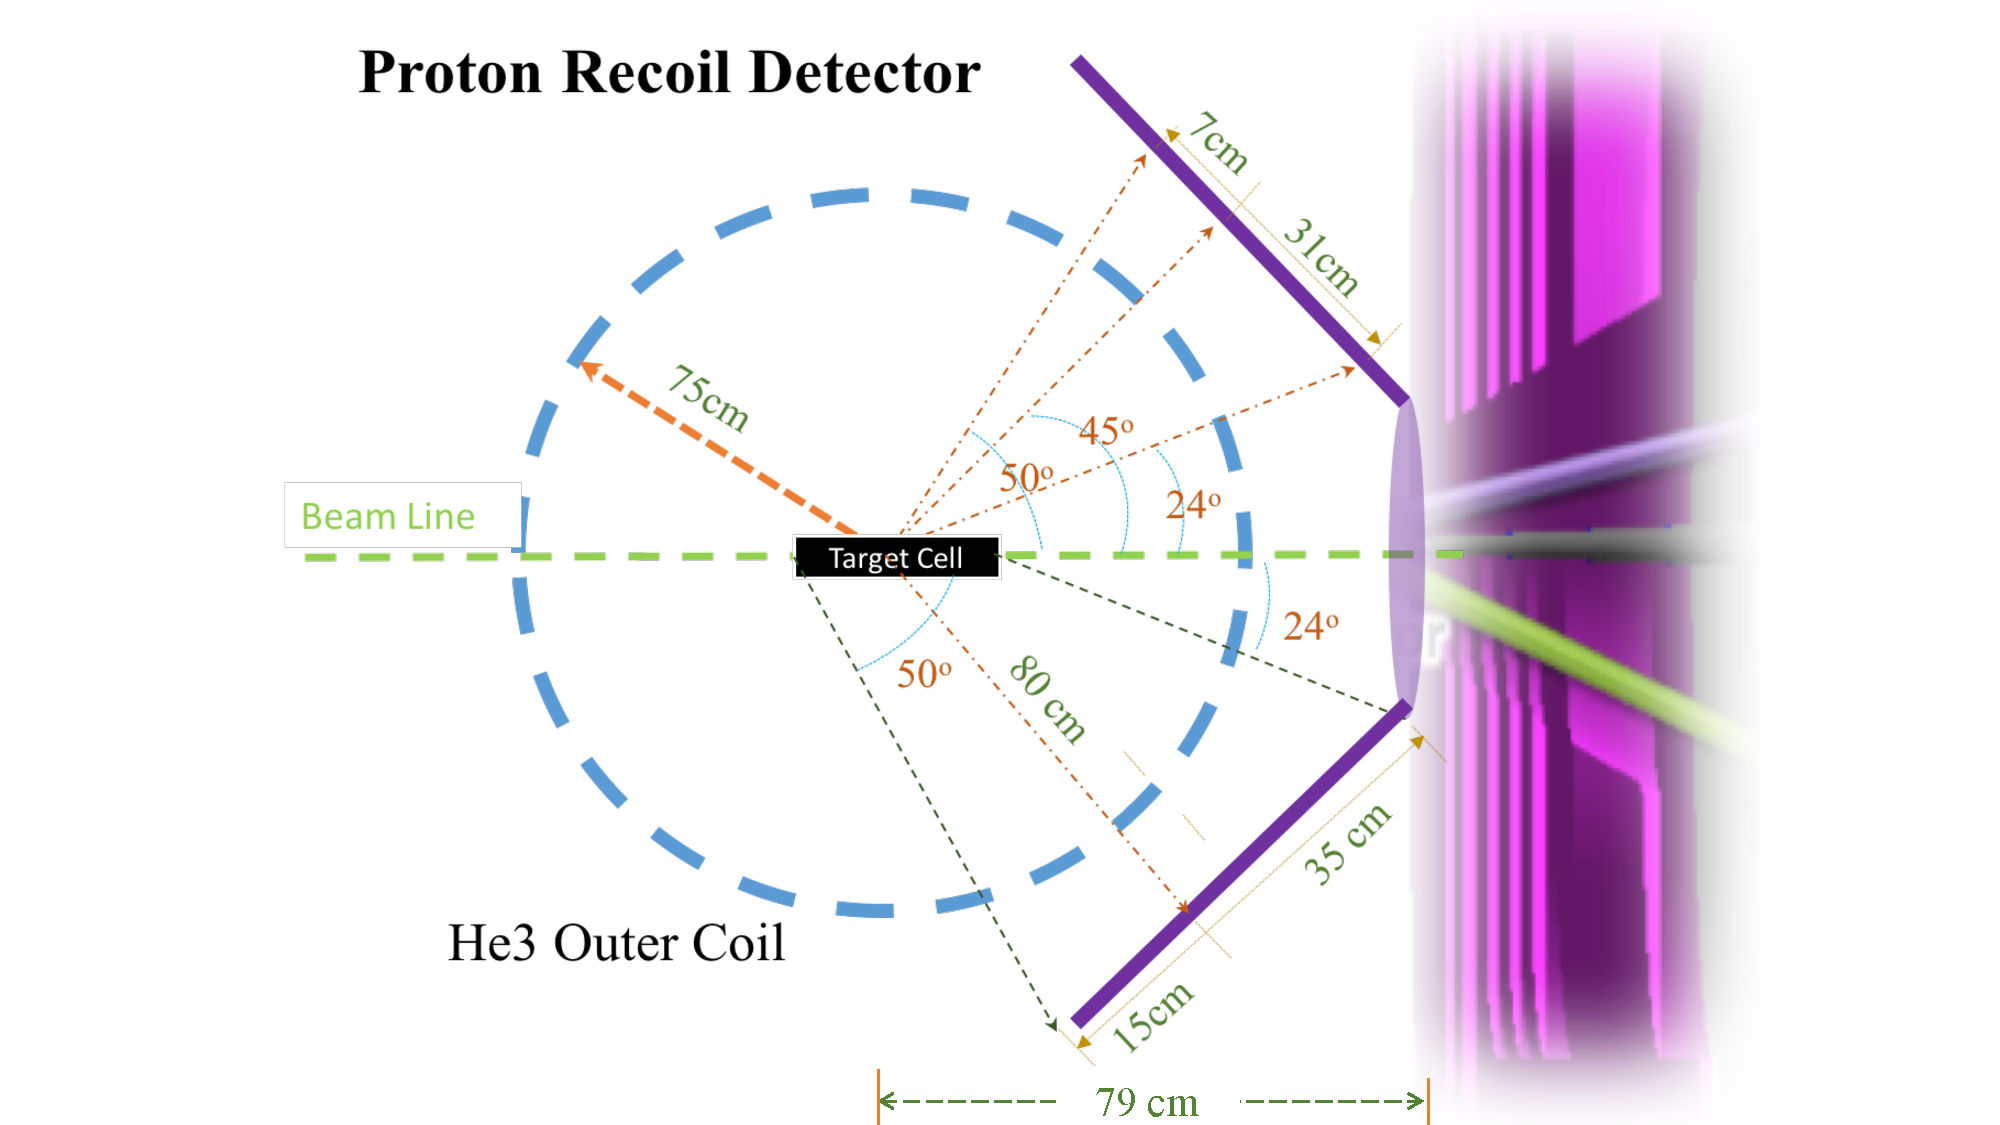
\includegraphics[width=0.7\textwidth]{./figures/prd_solid.pdf}
   \caption[Scheme of the new proton recoil detector ]{\footnotesize{Scheme of
       the new proton recoil detector. Such a cone-shape detector will be
       placed outside the outer Helmholtz coil of the $\mathrm{^{3}He}$ target
       system, covering polar angles from 24$^{\circ}$ to 50$^{\circ}$ and with
       2$\pi$ acceptance in azimuthal angle. We assume the detector plane
       to be tilted by -45$^{\circ}$ w.r.t. the beam direction with the
       vertical distance from the target center to the detector to be around
       80~cm. In this setting, the length of the detector is about 38~cm, and
       considering the target cell is 20~cm long, we extend the length to be
       50~cm. The inner and outer radius to be near 32~cm and 67~cm,
       respectively. The rough location of the solenoid is also indicated here. Note that lengths and locations are rough estimated, and the scales of angles and length are not proportional to the real scales.}}
   \label{prd_concept}
 \end{center}
\end{figure}
As shown in Fig.~\ref{prd_concept}, a new proton recoil detector (PRD) will be
placed right outside the $\mathrm{^{3}He}$ target system where the radius of
the outer Helmholtz coil is about 75~cm. The PRD will need to cover the polar
angle from 24$^{\circ}$ to 50$^{\circ}$ and provide full acceptance in
azimuthal angle. To minimize the detector area, the detector plane is tilted by
-45$^{\circ}$ along the beam direction and the vertical distance from the plane
to the target center is about 80~cm. After taking into account that the target
cell is 20~cm long, we require the length of the detector to be 50 cm, and its
inner and outer radii to be 32 cm and 67 cm, respectively.

To successfully select protons, we require the timing resolution of the
detector to be better than 60~ps, as discussed in Section 2.3. Since the
detector is close to the target and will suffer a huge background of low energy
particles, particularly low energy electrons, the detector will be divided
into fine segments to avoid pile-up of background signals. In addition, a thin
aluminum sheet of $\sim$4.5~mm thickness in front of the detector should be
able to block most of low energy particles. The rough angular information
provided by this detector will be helpful to further reject
background and isolate protons during the offline data analysis when
reconstructing missing mass and momentum.

\subsection{Scintillating Fiber Tracker}

One of the good candidates for the PRD is a scintillating fiber tracker
(SFT)~\cite{sft_zye}. Scintillating fibers (SciFi) have now been largely used
in experiments of particle physics because of its fast timing response and
flexibility, and several commercial manufacturers are able to produce high
quality fibers and at relatively low prices. Instead of using traditional large
paddles, we can construct the PRD by grouping SciFi in arrays and form the
detector planes.  With two planes of fibers at perpendicular directions, the
PRD can also provide position information by determining which fiber is fired
in each plane. A 1-mm round fiber is able to provide a 0.5~mm position
resolution and with a distance of 80~cm away from the target center, the
angular resolution can be better than 0.5~mrad, which can be essential to
further isolate protons and reduce background. On top of that, the SciFi is
highly segmented so the rate of random low energy background particles hitting
on a single fiber can be largely minimized, and the pile-up effect should be
significantly reduced compared with large area scintillator paddles.

We will choose silicon photo-multipliers (SiPM) as the photon-detectors to
collect light produced in the fibers. SiPM is idea for low-photon-number
counting since the light yield produced by a SciFi is not as strong as one
produced in a thin scintillator paddle. It is also not sensitive to magnetic
field, while the PRD will be placed in between the target system and the SoLID
magnet which both have strong magnetic field. Besides, there will be a lot of
read out channels and the price of SiPM is low enough to make the new detector
affordable.  The combination of SciFi and SiPM will make the PRD a very compact
detector which is very important since the space between the target system and
the solenoid magnet is limited.

A prototype project, funded by JSA postdoctoral fellow award \cite{sft_zye},
has been under development and we expect to build a small SFT and test its
performance near a target system with electron beam at JLab.

%\subsection{GEANT4 Simulation}


\newpage
%\begin{thebibliography}{99}
\clearpage
\begin{thebibliography}{}

\bibitem{solid:e12-10-006} 
  Approved SoLID SIDIS experiment E12-10-006,\\
  "Target Single Spin Asymmetry in Semi-Inclusive Deep-Inelastic $(e,e'\pi^{\pm}$' Reaction on a Transversely Polarized $\mathrm{^{3}He}$ Target at 11 GeV",\\
$https://www.jlab.org/exp\_prog/proposals/14/E12-10-006A.pdf$

\bibitem{solid_pcdr} 
  SoLID Collaboration, ``Solenoial Large Intensity Device Preliminary Conceptual Design Report,''
  $http://hallaweb.jlab.org/12GeV/SoLID/files/solid\_precdr.pdf$
  
\bibitem{hermes10} A. Airapetian, Phys. Lett. {\bf B 682} (2010) 345-350,
  arXiv:0907.2596 [hep-ex].
\bibitem{atpi39} PR12-12-005:
D. Dutta, D. Gaskell, W. Hersman, G.M. Huber, et al., ``The Longitudinal
Photon, Transverse Nucleon, Single-Spin Asymmetry in Exclusive Pion
Production''.
\bibitem{Di00} M. Diehl, Contribution to the eRHIC White Paper,
arXiv:hep-ph/0010200.
\bibitem{Co97} J.C. Collins, L. Frankfurt, M. Strikman, Phys. Rev. D {\bf 56}
  (1997) 2982.
\bibitem{Go01} K. Goeke, M.V. Polyakov, M. Vanderhaeghen,
  Prog. Part. Nucl. Phys. {\bf 47} (2001) 401-515.
\bibitem{Ra00} A.V. Radyushkin, arXiv:hep-ph/0101225.
\bibitem{Th01} A.W. Thomas, W. Weise, ``The Structure of the Nucleon'',
  J. Wiley-VCH, 2001.
\bibitem{Ma69} R.E. Marshak, Riazuddin, C.P. Ryan, ``Theory of Weak
  Interactions in Particle Physics'', J. Wiley, 1969.
\bibitem{Pe00} M. Penttinen, M.V. Polyakov, K. Goeke, Phys. Rev. C {\bf 62}
  (2000) 014024 1-11.
\bibitem{Be01} A.V. Belitsky, D. Mueller, Phys. Lett. {\bf B 513}
  (2001) 349-360.
\bibitem{Fr99} L.L. Frankfurt, P.V. Pobylitsa, M.V. Polyakov, M. Strikman,
  Phys. Rev. D {\bf 60} (1999) 014010 1-11.
\bibitem{Va99} M. Vanderhaeghen, P.A.M. Guichon, M. Guidal, Phys. Rev. D 
  {\bf 60} (1999) 094017 1-28.
\bibitem{Fr00} L.L. Frankfurt, M.V. Polyakov, M. Strikman, M. Vanderhaeghen,
  Phys. Rev. Lett. {\bf 84} (2000) 2589-2592.
\bibitem{belitsky} A.V. Belitsky, CIPANP 2003 proceedings.  arXiv:
  hep-ph/0307256.
\bibitem{Ma99} L. Mankiewicz, G. Piller, A. Radyushkin, Eur. Phys. J. {\bf C
    10} (1999) 307-312.
\bibitem{Ca90} C.E. Carlson, J. Milana, Phys. Rev. Lett. {\bf 65} (1990) 1717.
\bibitem{12GeV} E12-06-101, ``Measurement of the Charged Pion Form Factor to
  High $Q^2$'', G.M. Huber, D. Gaskell, spokespersons.
\bibitem{Go10} S.~V.~Goloskokov and P.~Kroll, Eur.\ Phys.\ J.\ C {\bf 65},
  137 (2010), arXiv:0906.0460 [hep-ph].
\bibitem{Di05} M. Diehl, S. Sapeta, Eur. Phys. J. C {\bf 41} (2005) 515,
  arXiv:hep-ph/0503023.
\bibitem{GoPC} S.~V.~Goloskokov and P.~Kroll, private communications 2009-12.
\bibitem{Fpi2} H.P. Blok, et al., Phys. Rev. C {\bf 78} (2008) 045202.
\bibitem{clas} pCDR for the Science and Experimental Equipment for the 12 GeV
  Upgrade of CEBAF, June, 2004.\\
V. Burkert et al., PAC18 Review of the Science Driving the 12 GeV Upgrade, 
  July, 2000.
\bibitem{3hepol1}J. L. Friar et al., Phys. Rev. C 42, (1990) 2310; C. Ciofi
degli Atti, and S. Scopetta, Phys. Lett. {\bf B404}, (1997) 223; R.W. Schulze
and P.U. Sauer, Phys. Rev. {\bf C56} (1997) 2293; F. Bissey, A.W. Thomas, and
I.R. Afnan, Phys. Rev. {\bf C64}, (2001) 024004.

\bibitem{solid:e12-11-007} 
  Approved SoLID SIDIS experiment E12-11-007,\\
"Asymmetries in Semi-Inclusive Deep-Inelastic  $(e,e'\pi^{\pm}$ Reactions on a Longitudinally Polarized $\mathrm{^{3}He}$ Target at 8.8 and 11 GeV ",\\
$https://www.jlab.org/exp_prog/PACpage/PAC37/proposals/Proposals/New\%20Proposals/PR-11-007.pdf$

\bibitem{solid:e12-11-108} 
  Approved SoLID SIDIS experiment E12-11-108,\\
"Target Single Spin Asymmetry in Semi-Inclusive Deep-Inelastic $(e,e'\pi^{\pm}$ Reactions on a Transversely Polarized Proton Target",\\
$https://www.jlab.org/exp\_prog/proposals/11/PR12-11-108.pdf$

\bibitem{solid:e12-12-006} 
  Approved SoLID J/$\mathrm{\psi}$ experiment E12-12-006A,\\
  "Near Threshold Electroproduction of J/$\mathrm{\psi}$ at 11 GeV",\\
$https://www.jlab.org/exp_prog/proposals/12/PR12-12-006.pdf$

\bibitem{solid:e12-11-008A}
   Approved SoLID SIDIS experiment E12-11-108A,\\
"Target Single Spin Asymmetry Measurements in the Inclusive Deep-Inelastic $vec{N}(e,e')$ Reaction on Transversely Polarized Proton and Neutron ($\mathrm{^{3}He}$) Targets using the SoLID Spectrometer "\\
$https://www.jlab.org/exp_prog/proposals/14/E12-11-108A_E12-10-006A.pdf$

\bibitem{solid:e12-10-006A} 
  Approved SoLID SIDIS experiment E12-10-006A,\\
  "Dihadron Electroproduction in DIS with  Transversely Polarized $\mathrm{^{3}He}$ Target at 11 and 8.8 GeV",\\
$https://www.jlab.org/exp_prog/proposals/14/E12-10-006A.pdf$

\bibitem{solid:e12-10-007} 
  Approved SoLID PVDIS experiment E12-10-007,\\
  "Precision Measurement of Parity-violation in Deep Inelastic Scattering Over a Broad Kinematic Range",\\
  $https://www.jlab.org/exp\_prog/PACpage/PAC37/proposals/Proposals/Previously\%20Approved/E12-10-007.pdf$


\bibitem{vr}	        T.~Vrancx and J.~Ryckebusch., Phys.~Rev.~\textbf{C89}, 025203 (2014).
\bibitem{gmhuber-2}	G.~M.~Huber $\textit{et}$ $\textit{al}$., Phys.~Rev.~\textbf{C91}, 015202 (2015).
\bibitem{gmhuber}	H.~Blok $\textit{et}$ $\textit{al}$., Phys.~Rev.~\textbf{C78}, 045202 (2008).
\bibitem{hallc-1}	T.~Horn $\textit{et}$ $\textit{al}$., Phys.~Rev.~Lett~\textbf{97}, 192001 (2006).
\bibitem{hallc-2}	T.~Horn $\textit{et}$ $\textit{al}$., Phys.~Rev.~\textbf{C78}, 058201 (2008).
\bibitem{park}	        http://clas.sinp.msu.ru/cgi-bin/jlab/db.cgi?eid=36;search=on
\bibitem{hermes}	A.~Airapetian $\textit{et}$ $\textit{al}$., Phys.~Lett.~B.~\textbf{659}, (2008).
\bibitem{frankfurt}	L.~L.~Frankfurt $\textit{et}$ $\textit{al}$., Phys.~Rev.~Lett.~\textbf{84}, 2589 (2000).


\bibitem{sft_zye} Z. Ye, A Prototype Project of a new Scintillating Fiber Tracker, 2014 JSA Postdoc Fellowship,\\ "$https://userweb.jlab.org/~yez/Work/SFT/SFT\_prop.pdf$"
\end{thebibliography}

%\end{thebibliography}

\end{document}
